\documentclass[]{article}
\usepackage{lmodern}
\usepackage{amssymb,amsmath}
\usepackage{ifxetex,ifluatex}
\usepackage{fixltx2e} % provides \textsubscript
\ifnum 0\ifxetex 1\fi\ifluatex 1\fi=0 % if pdftex
  \usepackage[T1]{fontenc}
  \usepackage[utf8]{inputenc}
\else % if luatex or xelatex
  \ifxetex
    \usepackage{mathspec}
  \else
    \usepackage{fontspec}
  \fi
  \defaultfontfeatures{Ligatures=TeX,Scale=MatchLowercase}
\fi
% use upquote if available, for straight quotes in verbatim environments
\IfFileExists{upquote.sty}{\usepackage{upquote}}{}
% use microtype if available
\IfFileExists{microtype.sty}{%
\usepackage{microtype}
\UseMicrotypeSet[protrusion]{basicmath} % disable protrusion for tt fonts
}{}
\usepackage[margin=1in]{geometry}
\usepackage{hyperref}
\hypersetup{unicode=true,
            pdftitle={Supplementary document},
            pdfauthor={Anatoly Sorokin},
            pdfborder={0 0 0},
            breaklinks=true}
\urlstyle{same}  % don't use monospace font for urls
\usepackage{color}
\usepackage{fancyvrb}
\newcommand{\VerbBar}{|}
\newcommand{\VERB}{\Verb[commandchars=\\\{\}]}
\DefineVerbatimEnvironment{Highlighting}{Verbatim}{commandchars=\\\{\}}
% Add ',fontsize=\small' for more characters per line
\usepackage{framed}
\definecolor{shadecolor}{RGB}{248,248,248}
\newenvironment{Shaded}{\begin{snugshade}}{\end{snugshade}}
\newcommand{\KeywordTok}[1]{\textcolor[rgb]{0.13,0.29,0.53}{\textbf{#1}}}
\newcommand{\DataTypeTok}[1]{\textcolor[rgb]{0.13,0.29,0.53}{#1}}
\newcommand{\DecValTok}[1]{\textcolor[rgb]{0.00,0.00,0.81}{#1}}
\newcommand{\BaseNTok}[1]{\textcolor[rgb]{0.00,0.00,0.81}{#1}}
\newcommand{\FloatTok}[1]{\textcolor[rgb]{0.00,0.00,0.81}{#1}}
\newcommand{\ConstantTok}[1]{\textcolor[rgb]{0.00,0.00,0.00}{#1}}
\newcommand{\CharTok}[1]{\textcolor[rgb]{0.31,0.60,0.02}{#1}}
\newcommand{\SpecialCharTok}[1]{\textcolor[rgb]{0.00,0.00,0.00}{#1}}
\newcommand{\StringTok}[1]{\textcolor[rgb]{0.31,0.60,0.02}{#1}}
\newcommand{\VerbatimStringTok}[1]{\textcolor[rgb]{0.31,0.60,0.02}{#1}}
\newcommand{\SpecialStringTok}[1]{\textcolor[rgb]{0.31,0.60,0.02}{#1}}
\newcommand{\ImportTok}[1]{#1}
\newcommand{\CommentTok}[1]{\textcolor[rgb]{0.56,0.35,0.01}{\textit{#1}}}
\newcommand{\DocumentationTok}[1]{\textcolor[rgb]{0.56,0.35,0.01}{\textbf{\textit{#1}}}}
\newcommand{\AnnotationTok}[1]{\textcolor[rgb]{0.56,0.35,0.01}{\textbf{\textit{#1}}}}
\newcommand{\CommentVarTok}[1]{\textcolor[rgb]{0.56,0.35,0.01}{\textbf{\textit{#1}}}}
\newcommand{\OtherTok}[1]{\textcolor[rgb]{0.56,0.35,0.01}{#1}}
\newcommand{\FunctionTok}[1]{\textcolor[rgb]{0.00,0.00,0.00}{#1}}
\newcommand{\VariableTok}[1]{\textcolor[rgb]{0.00,0.00,0.00}{#1}}
\newcommand{\ControlFlowTok}[1]{\textcolor[rgb]{0.13,0.29,0.53}{\textbf{#1}}}
\newcommand{\OperatorTok}[1]{\textcolor[rgb]{0.81,0.36,0.00}{\textbf{#1}}}
\newcommand{\BuiltInTok}[1]{#1}
\newcommand{\ExtensionTok}[1]{#1}
\newcommand{\PreprocessorTok}[1]{\textcolor[rgb]{0.56,0.35,0.01}{\textit{#1}}}
\newcommand{\AttributeTok}[1]{\textcolor[rgb]{0.77,0.63,0.00}{#1}}
\newcommand{\RegionMarkerTok}[1]{#1}
\newcommand{\InformationTok}[1]{\textcolor[rgb]{0.56,0.35,0.01}{\textbf{\textit{#1}}}}
\newcommand{\WarningTok}[1]{\textcolor[rgb]{0.56,0.35,0.01}{\textbf{\textit{#1}}}}
\newcommand{\AlertTok}[1]{\textcolor[rgb]{0.94,0.16,0.16}{#1}}
\newcommand{\ErrorTok}[1]{\textcolor[rgb]{0.64,0.00,0.00}{\textbf{#1}}}
\newcommand{\NormalTok}[1]{#1}
\usepackage{longtable,booktabs}
\usepackage{graphicx,grffile}
\makeatletter
\def\maxwidth{\ifdim\Gin@nat@width>\linewidth\linewidth\else\Gin@nat@width\fi}
\def\maxheight{\ifdim\Gin@nat@height>\textheight\textheight\else\Gin@nat@height\fi}
\makeatother
% Scale images if necessary, so that they will not overflow the page
% margins by default, and it is still possible to overwrite the defaults
% using explicit options in \includegraphics[width, height, ...]{}
\setkeys{Gin}{width=\maxwidth,height=\maxheight,keepaspectratio}
\IfFileExists{parskip.sty}{%
\usepackage{parskip}
}{% else
\setlength{\parindent}{0pt}
\setlength{\parskip}{6pt plus 2pt minus 1pt}
}
\setlength{\emergencystretch}{3em}  % prevent overfull lines
\providecommand{\tightlist}{%
  \setlength{\itemsep}{0pt}\setlength{\parskip}{0pt}}
\setcounter{secnumdepth}{5}
% Redefines (sub)paragraphs to behave more like sections
\ifx\paragraph\undefined\else
\let\oldparagraph\paragraph
\renewcommand{\paragraph}[1]{\oldparagraph{#1}\mbox{}}
\fi
\ifx\subparagraph\undefined\else
\let\oldsubparagraph\subparagraph
\renewcommand{\subparagraph}[1]{\oldsubparagraph{#1}\mbox{}}
\fi

%%% Use protect on footnotes to avoid problems with footnotes in titles
\let\rmarkdownfootnote\footnote%
\def\footnote{\protect\rmarkdownfootnote}

%%% Change title format to be more compact
\usepackage{titling}

% Create subtitle command for use in maketitle
\newcommand{\subtitle}[1]{
  \posttitle{
    \begin{center}\large#1\end{center}
    }
}

\setlength{\droptitle}{-2em}
  \title{Supplementary document}
  \pretitle{\vspace{\droptitle}\centering\huge}
  \posttitle{\par}
  \author{Anatoly Sorokin}
  \preauthor{\centering\large\emph}
  \postauthor{\par}
  \predate{\centering\large\emph}
  \postdate{\par}
  \date{6/15/2017}

\usepackage[OT1]{fontenc}
\usepackage[utf8]{inputenc} % set input encoding (not needed with XeLaTeX)
\usepackage[english]{babel}
\usepackage{grffile}
\usepackage{rotating}
\usepackage{caption}
\usepackage{longtable}
\usepackage{lscape}
\usepackage{float}

\usepackage{color}
\definecolor{lightgray}{gray}{0.95}

\usepackage{listings}
\lstset{
language=R,                			% choose the language of the code
basicstyle=\verbatim@font,      % the size of the fonts that are used for the code
%breaklines=true,                % sets automatic line breaking
%breakatwhitespace=true,					%force breaks at white space
showspaces=false,								%don't display funky characters where there are spaces
showstringspaces=false,					%show spaces within strings
columns=fullflexible,						%makes character spacing nice
,captionpos=t,tabsize=3,frame=tb,
%   keywordstyle=\color{blue},
%   commentstyle=\color{gray},stringstyle=\color{red},
   numbers=right,
   numberstyle=\small,
   numbersep=5pt,breaklines=true,showstringspaces=false,
   basicstyle=\footnotesize,emph={label},breakatwhitespace=false,escapeinside={`}{`}
}
\floatstyle{ruled}
\newfloat{program}{thp}{lop}
\floatname{program}{Listing}

\begin{document}
\maketitle

{
\setcounter{tocdepth}{2}
\tableofcontents
}
\section{Load the data}\label{load-the-data}

Thermo RAW files were converted into mzXML by ReAdW.201510.xcalibur.exe
application. After that we load mzXML file into R with help of XCMS
package and convert it into MZ table:

\begin{Shaded}
\begin{Highlighting}[]
\NormalTok{  xraw <-}\StringTok{ }\KeywordTok{xcmsRaw}\NormalTok{(}\KeywordTok{paste0}\NormalTok{(path,FName))}
\NormalTok{  p<-}\KeywordTok{makePeaks}\NormalTok{(xraw)}
\NormalTok{  scanLen <-}\StringTok{ }\KeywordTok{max}\NormalTok{(p}\OperatorTok{$}\NormalTok{scan)}
\end{Highlighting}
\end{Shaded}

As a result we have table with 5 columns: ``mz'', ``intensity'',
``ion'', ``time'', ``scan'' to store m/z, intensity, time of scan and
its number. Column ``ion'' is reserved for ID of the feature, obtained
with further analysis.

\section{Feature selection}\label{feature-selection}

The algorithm process data in the MZ table in intensity descending
order, so whenever it stops we can be sure that we identify most
important features in the data.

At the first step algorithm selects row with highest intensity, which is
not assigned to any feature yet, and take its m/z value as proposed
feature position:

\begin{Shaded}
\begin{Highlighting}[]
\NormalTok{  idx<-}\KeywordTok{which}\NormalTok{(}\KeywordTok{is.na}\NormalTok{(p}\OperatorTok{$}\NormalTok{ion))}
\NormalTok{  cP<-}\KeywordTok{which.max}\NormalTok{(p}\OperatorTok{$}\NormalTok{intensity[idx])}
\NormalTok{  ionI<-idx[cP]}
\NormalTok{  maxMZ<-p}\OperatorTok{$}\NormalTok{mz[ionI]}
\end{Highlighting}
\end{Shaded}

The selected row represents the peak with m/z=844.6437 of the scan N=45
taken at time 59.4 sec:

\begin{Shaded}
\begin{Highlighting}[]
\KeywordTok{print}\NormalTok{(}\KeywordTok{getScanPlot}\NormalTok{(p[scan}\OperatorTok{==}\NormalTok{p}\OperatorTok{$}\NormalTok{scan[ionI]]))}
\end{Highlighting}
\end{Shaded}

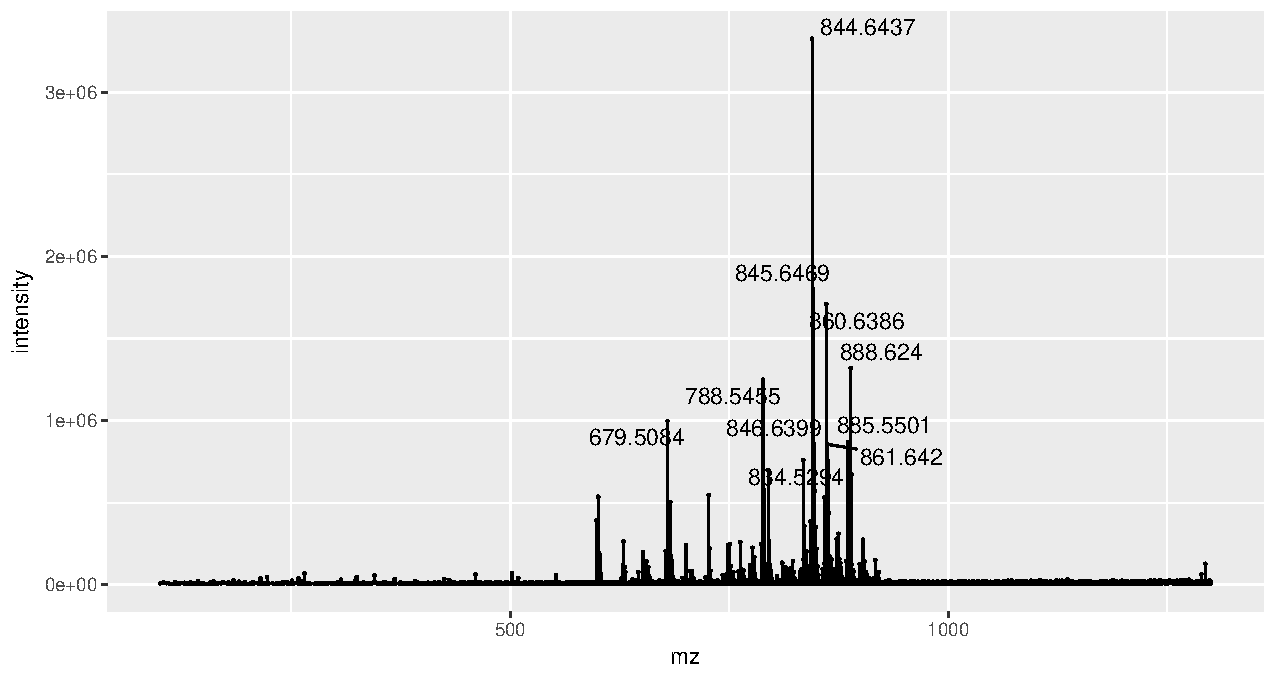
\includegraphics{Supplementary_document_files/figure-latex/ion.plots-1.pdf}

Now we collect all signals in the vicinity (50 ppm) of the selected m/z
value and analyze how they drift with time:

\begin{Shaded}
\begin{Highlighting}[]
\NormalTok{  idx <-}\StringTok{ }\KeywordTok{which}\NormalTok{(}\KeywordTok{abs}\NormalTok{(p}\OperatorTok{$}\NormalTok{mz }\OperatorTok{-}\StringTok{ }\NormalTok{maxMZ) }\OperatorTok{<}\StringTok{ }\NormalTok{(ppm }\OperatorTok{*}\StringTok{ }\FloatTok{1e-6} \OperatorTok{*}\StringTok{ }\NormalTok{maxMZ))}
\NormalTok{  p. <-}\StringTok{ }\NormalTok{p[idx, ]}
\end{Highlighting}
\end{Shaded}

To separate feature from surrounding noise we cluster data in m/z domain
by hierarchical Ward clustering and select the most stable clusters with
dynamicTreeCut:

\begin{Shaded}
\begin{Highlighting}[]
\NormalTok{  dissim1 =}\StringTok{ }\KeywordTok{dist}\NormalTok{(p.}\OperatorTok{$}\NormalTok{mz)}
\NormalTok{  dendro1 <-}\StringTok{ }\KeywordTok{hclust}\NormalTok{(}\DataTypeTok{d =}\NormalTok{ dissim1, }\DataTypeTok{method =} \StringTok{'ward.D2'}\NormalTok{)}
\NormalTok{  ct1 <-}\StringTok{ }\KeywordTok{cutreeDynamic}\NormalTok{(}
\NormalTok{    dendro1,}
    \DataTypeTok{cutHeight =} \OtherTok{NULL}\NormalTok{,}
    \DataTypeTok{minClusterSize =} \DecValTok{30}\NormalTok{,}
    \DataTypeTok{method =} \StringTok{"hybrid"}\NormalTok{,}
    \DataTypeTok{deepSplit =} \DecValTok{0}\NormalTok{,}
    \DataTypeTok{pamStage =} \OtherTok{TRUE}\NormalTok{,}
    \DataTypeTok{distM =} \KeywordTok{as.matrix}\NormalTok{(dissim1),}
    \DataTypeTok{maxPamDist =} \DecValTok{0}\NormalTok{,}
    \DataTypeTok{verbose =} \DecValTok{0}
\NormalTok{  )}
\NormalTok{  cct1 <-}\StringTok{ }\NormalTok{ct1[}\KeywordTok{which.max}\NormalTok{(p.}\OperatorTok{$}\NormalTok{intensity)]}
\NormalTok{  id.}\DecValTok{1}\NormalTok{ <-}\StringTok{ }\NormalTok{idx[ct1 }\OperatorTok{==}\StringTok{ }\NormalTok{cct1]}
\NormalTok{  mz1 <-}\StringTok{ }\KeywordTok{median}\NormalTok{(p}\OperatorTok{$}\NormalTok{mz[id.}\DecValTok{1}\NormalTok{])}
\NormalTok{  p.}\OperatorTok{$}\NormalTok{color<-.pal[ct1}\OperatorTok{+}\DecValTok{1}\NormalTok{]}
\NormalTok{  rl <-}\StringTok{ }\KeywordTok{get_runLen}\NormalTok{(p}\OperatorTok{$}\NormalTok{scan[id.}\DecValTok{1}\NormalTok{], scanLen)}
\NormalTok{  p1<-}\KeywordTok{qplot}\NormalTok{(time,intensity,}\DataTypeTok{data =}\NormalTok{ p.,}\DataTypeTok{main=}\KeywordTok{paste0}\NormalTok{(}\StringTok{'mz'}\NormalTok{,maxMZ),}\DataTypeTok{log=}\StringTok{'y'}\NormalTok{,}\DataTypeTok{color=}\NormalTok{color)}
\NormalTok{  p2<-}\KeywordTok{qplot}\NormalTok{(time,mz,}\DataTypeTok{data =}\NormalTok{ p.,}\DataTypeTok{color=}\NormalTok{color)}
\NormalTok{  p3<-}\KeywordTok{qplot}\NormalTok{(mz,intensity,}\DataTypeTok{data =}\NormalTok{ p.,}\DataTypeTok{color=}\NormalTok{color)}
  \KeywordTok{print}\NormalTok{(}\KeywordTok{multiplot}\NormalTok{(p1, p2, p3, }\DataTypeTok{cols=}\DecValTok{1}\NormalTok{))}
\end{Highlighting}
\end{Shaded}

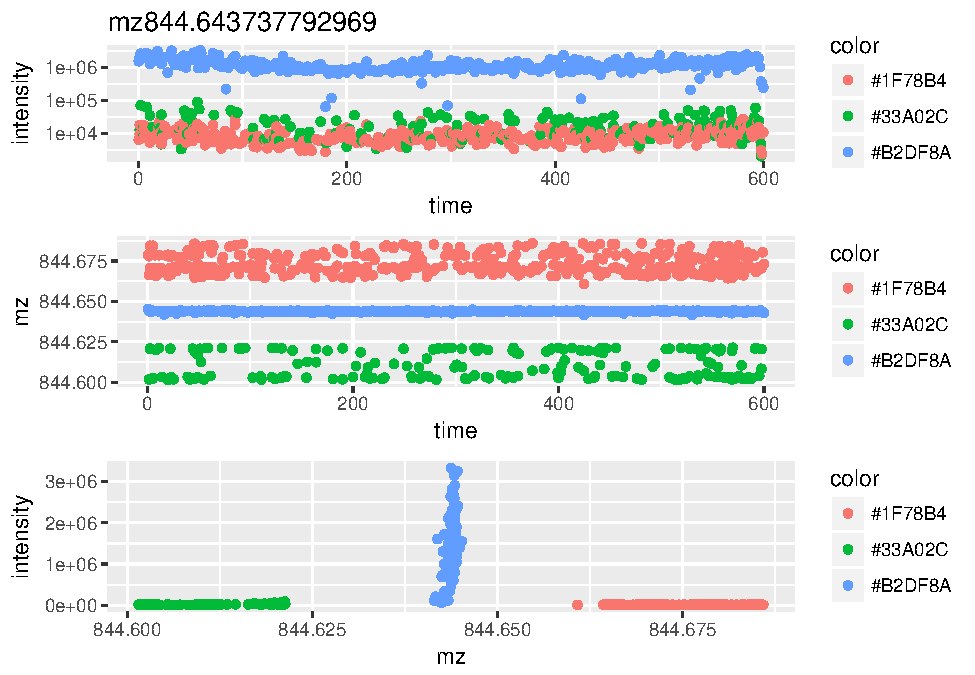
\includegraphics{Supplementary_document_files/figure-latex/cluster.mz-1.pdf}

\begin{verbatim}
## NULL
\end{verbatim}

It could be seen that selected m/z value forms a well separated cluster
as in m/z as in intensity domain, but this is not always the case. There
are peaks which could not be separated by such procedure, for example:

It could be seen that even in this case each feature visually represents
well separated line on the time vs m/z plot. So we can extract distinct
features by fitting data from cluster containing peak of highest
intensity to the linear function:

\begin{Shaded}
\begin{Highlighting}[]
\NormalTok{  l<-}\KeywordTok{lm}\NormalTok{(mz }\OperatorTok{~}\StringTok{ }\NormalTok{time, }\DataTypeTok{data =}\NormalTok{ p[id.}\DecValTok{1}\NormalTok{, ])}
\ControlFlowTok{if}\NormalTok{ (}\KeywordTok{all}\NormalTok{(}\OperatorTok{!}\KeywordTok{is.na}\NormalTok{(l}\OperatorTok{$}\NormalTok{coefficients))) \{}
\NormalTok{  op <-}\StringTok{ }\KeywordTok{par}\NormalTok{(}\DataTypeTok{mfrow =} \KeywordTok{c}\NormalTok{(}\DecValTok{2}\NormalTok{, }\DecValTok{2}\NormalTok{), }\DataTypeTok{oma =} \KeywordTok{c}\NormalTok{(}\DecValTok{0}\NormalTok{, }\DecValTok{0}\NormalTok{, }\DecValTok{2}\NormalTok{, }\DecValTok{0}\NormalTok{))}
  \KeywordTok{plot}\NormalTok{(l)}
  \KeywordTok{par}\NormalTok{(op)}
\NormalTok{\}}
\end{Highlighting}
\end{Shaded}

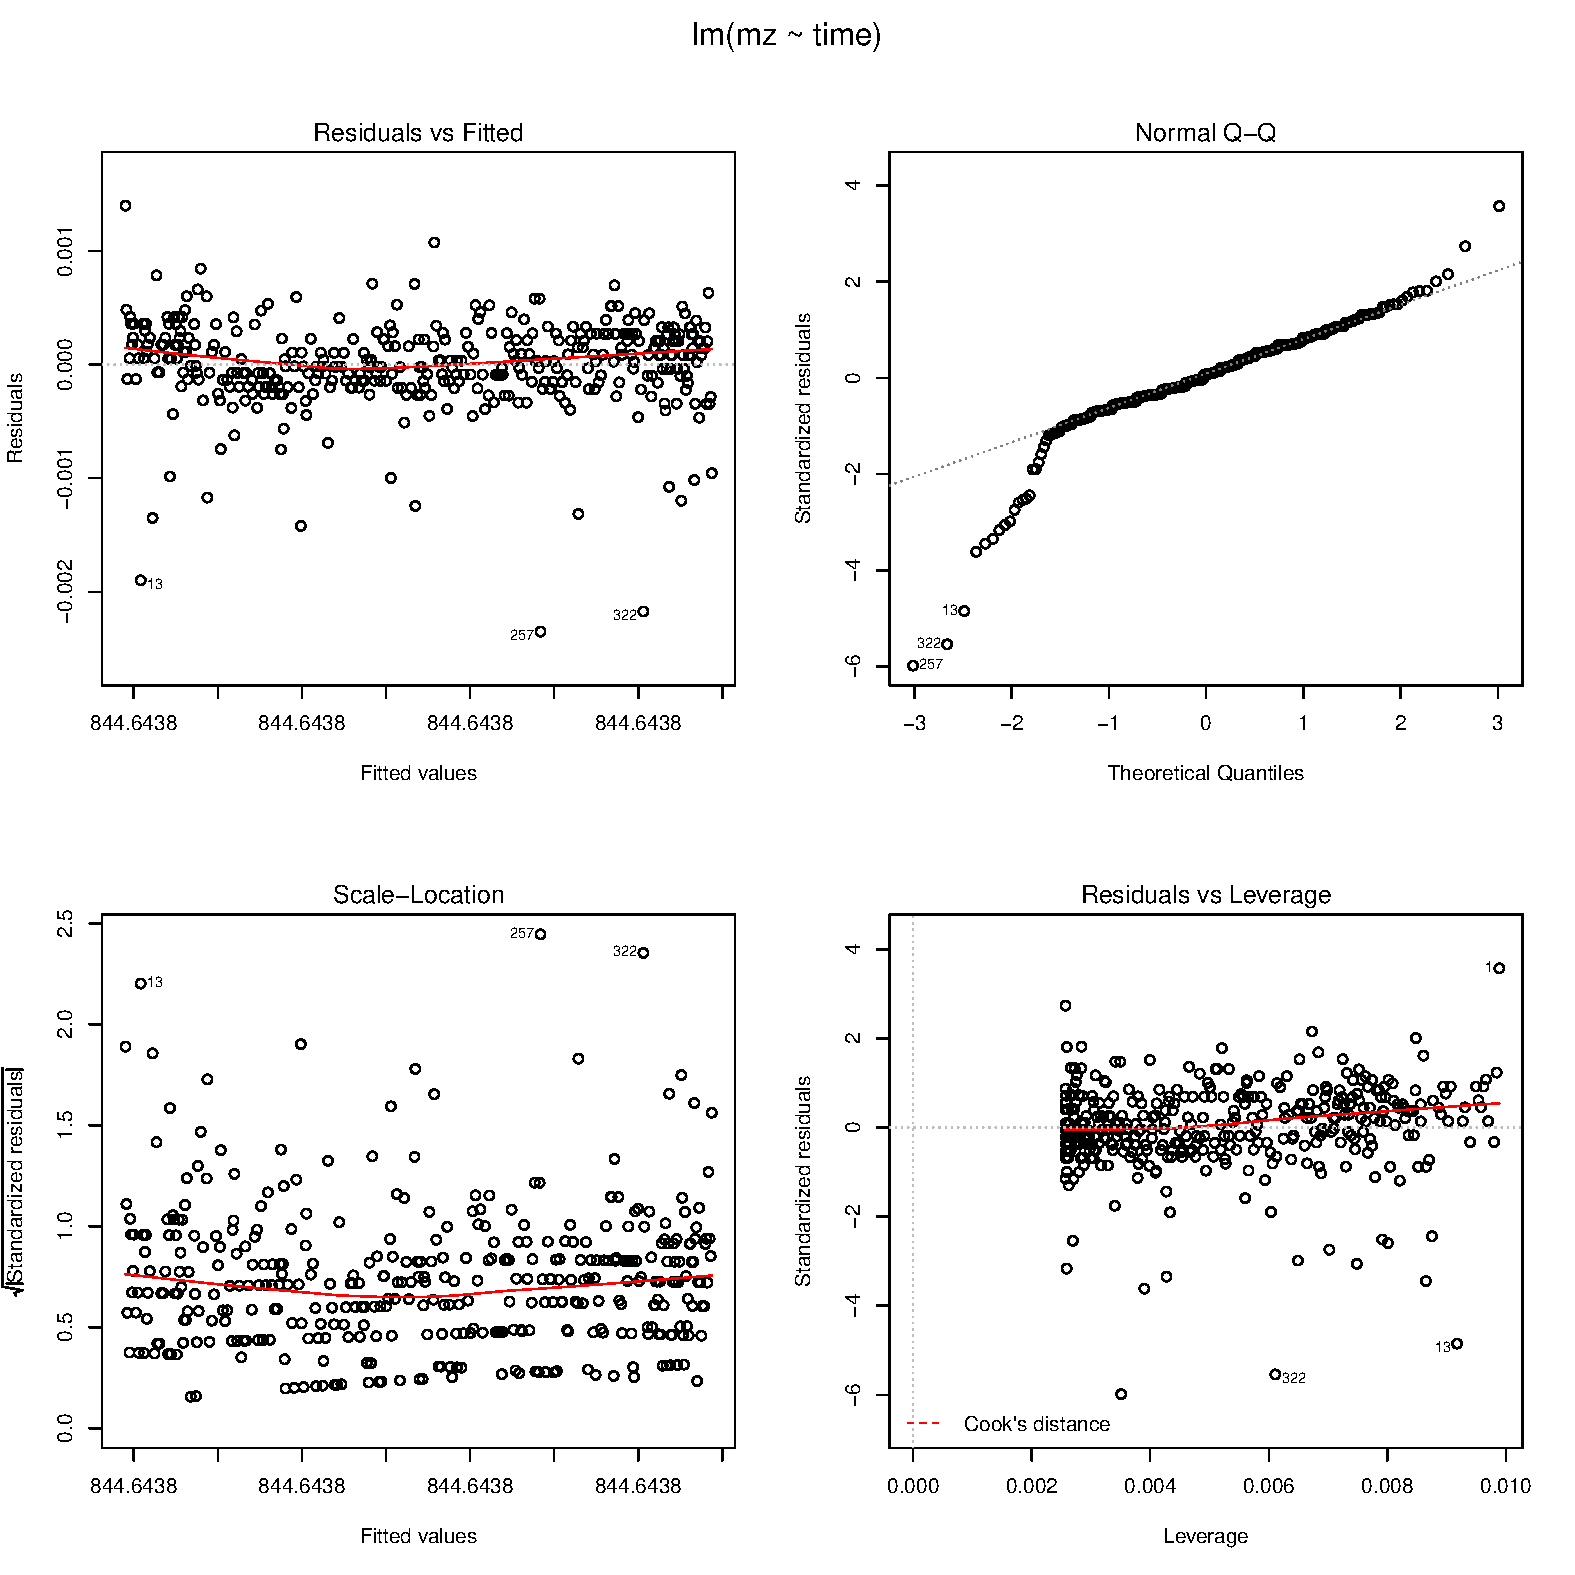
\includegraphics{Supplementary_document_files/figure-latex/fit.lin-1.pdf}

Now to incorporate to the feature all points, that form the line even if
they appear in different cluster we predict linear value for each point
in the selected interval and filter out all points with residuals higher
than two standard deviations:

\begin{Shaded}
\begin{Highlighting}[]
\ControlFlowTok{if}\NormalTok{ (}\KeywordTok{all}\NormalTok{(}\OperatorTok{!}\KeywordTok{is.na}\NormalTok{(l}\OperatorTok{$}\NormalTok{coefficients))) \{}
  \KeywordTok{range}\NormalTok{(l}\OperatorTok{$}\NormalTok{residuals[}\KeywordTok{abs}\NormalTok{(}\KeywordTok{rstandard}\NormalTok{(l)) }\OperatorTok{<=}\StringTok{ }\DecValTok{2}\NormalTok{]) ->}\StringTok{ }\NormalTok{bnd}
\NormalTok{  pl <-}\StringTok{ }\KeywordTok{predict}\NormalTok{(l, p.)}
\NormalTok{  rl <-}\StringTok{ }\NormalTok{p.}\OperatorTok{$}\NormalTok{mz }\OperatorTok{-}\StringTok{ }\NormalTok{pl}
\NormalTok{  idL <-}\StringTok{ }\KeywordTok{which}\NormalTok{(rl }\OperatorTok{>=}\StringTok{ }\NormalTok{bnd[}\DecValTok{1}\NormalTok{] }\OperatorTok{&}\StringTok{ }\NormalTok{rl }\OperatorTok{<=}\StringTok{ }\NormalTok{bnd[}\DecValTok{2}\NormalTok{])}
\NormalTok{  p5 =}\StringTok{ }\KeywordTok{qplot}\NormalTok{(}
\NormalTok{          time,}
\NormalTok{          mz,}
          \DataTypeTok{data =}\NormalTok{ p.[idL],}
          \DataTypeTok{color =}\NormalTok{ color,}
          \DataTypeTok{xlim =} \KeywordTok{range}\NormalTok{(p.}\OperatorTok{$}\NormalTok{time),}
          \DataTypeTok{ylim =} \KeywordTok{range}\NormalTok{(p.}\OperatorTok{$}\NormalTok{mz)}
\NormalTok{  )}
\NormalTok{  p6 =}\StringTok{ }\KeywordTok{qplot}\NormalTok{(time,}
\NormalTok{          mz,}
          \DataTypeTok{data =}\NormalTok{ p.,}
          \DataTypeTok{color =}\NormalTok{ color) }\OperatorTok{+}
\StringTok{      }\KeywordTok{geom_abline}\NormalTok{(}\DataTypeTok{intercept =}\NormalTok{ l}\OperatorTok{$}\NormalTok{coefficients[}\DecValTok{1}\NormalTok{],}
          \DataTypeTok{slope =}\NormalTok{ l}\OperatorTok{$}\NormalTok{coefficients[}\DecValTok{2}\NormalTok{])}
  
\NormalTok{  p.}\OperatorTok{$}\NormalTok{resPPM<-rl}\OperatorTok{*}\FloatTok{1e6}\OperatorTok{/}\NormalTok{l}\OperatorTok{$}\NormalTok{coefficients[}\DecValTok{1}\NormalTok{]}
\NormalTok{  p7<-}\KeywordTok{qplot}\NormalTok{(resPPM,}\DataTypeTok{data=}\NormalTok{p.[idL],}
            \DataTypeTok{binwidth=}\NormalTok{binwidth,}\DataTypeTok{color=}\NormalTok{color)}\OperatorTok{+}
\StringTok{    }\KeywordTok{stat_function}\NormalTok{(}\DataTypeTok{fun =} \ControlFlowTok{function}\NormalTok{(x, mean, sd, n, bw)\{}
      \KeywordTok{dnorm}\NormalTok{(}\DataTypeTok{x =}\NormalTok{ x, }\DataTypeTok{mean =}\NormalTok{ mean, }\DataTypeTok{sd =}\NormalTok{ sd) }\OperatorTok{*}\StringTok{ }\NormalTok{n }\OperatorTok{*}\StringTok{ }\NormalTok{bw}
\NormalTok{      \},}
      \DataTypeTok{args =} \KeywordTok{c}\NormalTok{(}\DataTypeTok{mean =} \KeywordTok{mean}\NormalTok{(p.}\OperatorTok{$}\NormalTok{resPPM[idL]), }
               \DataTypeTok{sd =} \KeywordTok{sd}\NormalTok{(p.}\OperatorTok{$}\NormalTok{resPPM[idL]), }
               \DataTypeTok{n =} \KeywordTok{length}\NormalTok{(idL), }
               \DataTypeTok{bw =}\NormalTok{ binwidth))}

  \KeywordTok{print}\NormalTok{(}\KeywordTok{multiplot}\NormalTok{(p5, p6, p7, }\DataTypeTok{cols =} \DecValTok{1}\NormalTok{))}
\NormalTok{\}}
\end{Highlighting}
\end{Shaded}

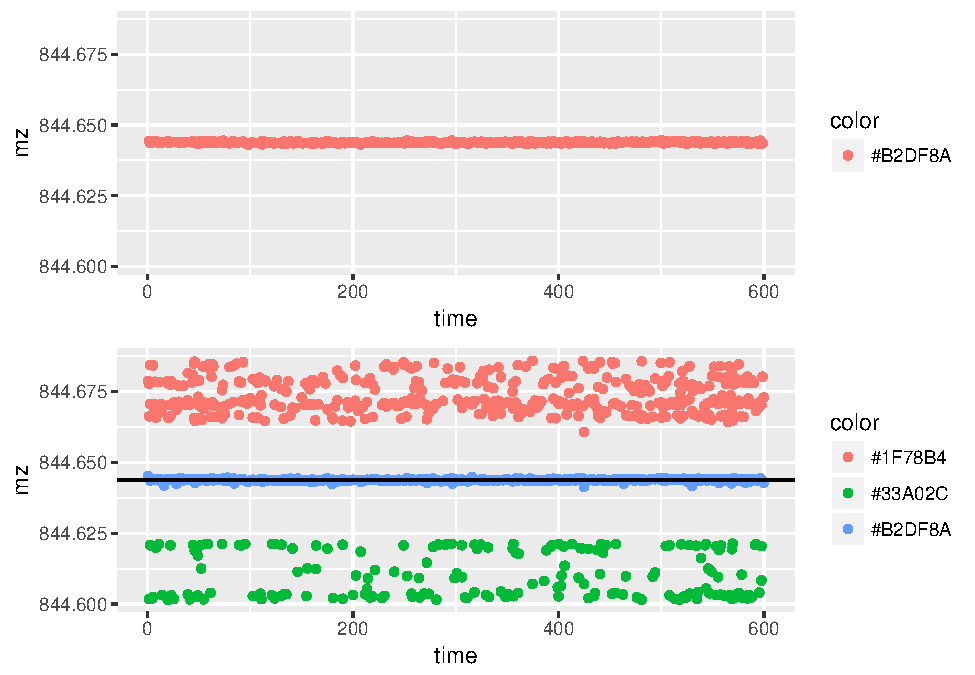
\includegraphics{Supplementary_document_files/figure-latex/filter.lm-1.pdf}

\begin{verbatim}
## NULL
\end{verbatim}

The fitted line will change due to rearrangement of the feature point
list, so we will repeat this step untill it converges, but no more than
50 times.

Final step of the algorithm is the quality control. The feature could be
too wide in m/z domain or it could eventually consists of several close
crests, it could contains several points from the same scan. As we
looking for continious features and rely on linear regression we will
remove from the list all features which is too short to produse reliable
regression. Only features wich contains more than 300 points in of more
than 100 consequtive scans will be preserved. High intensity bursting
ions should be analysed separately.

\section{MZ=651.477226}\label{mz651.477226}

\begin{Shaded}
\begin{Highlighting}[]
\NormalTok{  idx<-}\KeywordTok{which}\NormalTok{(}\KeywordTok{abs}\NormalTok{(p}\OperatorTok{$}\NormalTok{mz}\OperatorTok{-}\FloatTok{651.477226}\NormalTok{)}\OperatorTok{<}\FloatTok{1e-3}\NormalTok{)}
\NormalTok{  cP<-}\KeywordTok{which.max}\NormalTok{(p}\OperatorTok{$}\NormalTok{intensity[idx])}
\NormalTok{  ionI<-idx[cP]}
\NormalTok{  maxMZ<-p}\OperatorTok{$}\NormalTok{mz[ionI]}
\end{Highlighting}
\end{Shaded}

The selected row represents the peak with m/z=651.4775 of the scan N=42
taken at time 56.7 sec:

\begin{Shaded}
\begin{Highlighting}[]
\KeywordTok{print}\NormalTok{(}\KeywordTok{getScanPlot}\NormalTok{(p[scan}\OperatorTok{==}\NormalTok{p}\OperatorTok{$}\NormalTok{scan[ionI]]))}
\end{Highlighting}
\end{Shaded}

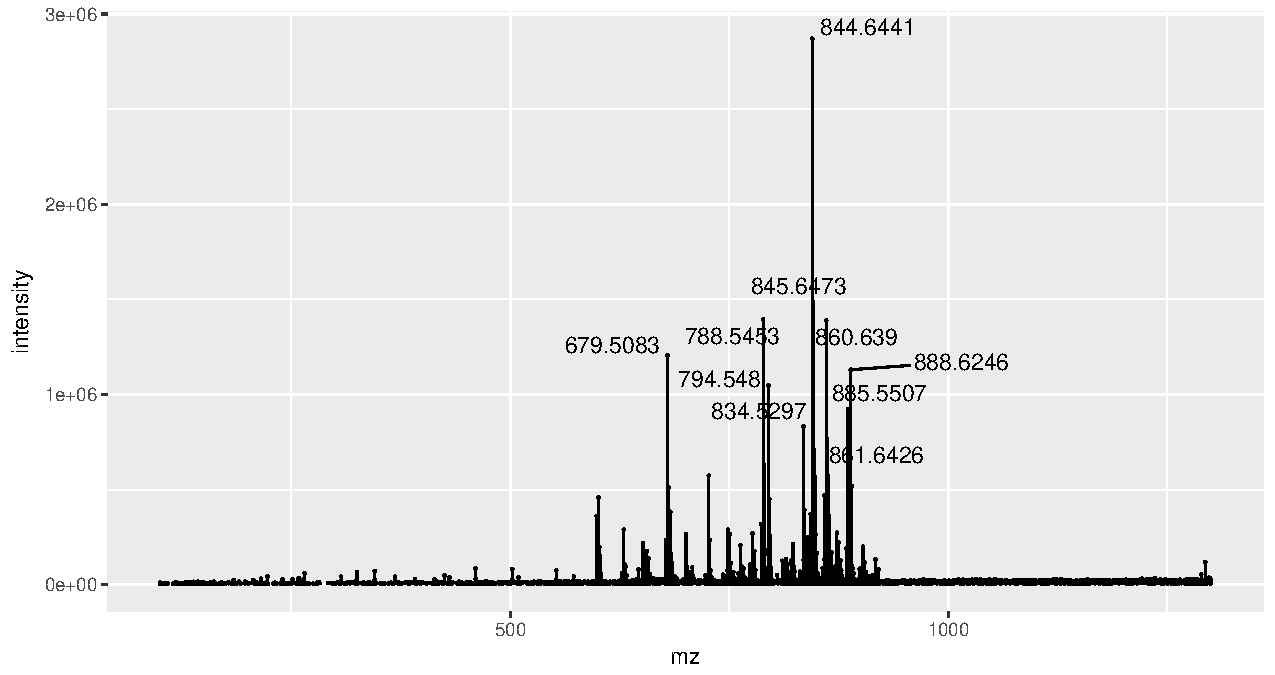
\includegraphics{Supplementary_document_files/figure-latex/ion.plots.651-1.pdf}

Now we collect all signals in the vicinity (50 ppm) of the selected m/z
value and analyze how they drift with time:

\begin{Shaded}
\begin{Highlighting}[]
\NormalTok{  idx <-}\StringTok{ }\KeywordTok{which}\NormalTok{(}\KeywordTok{abs}\NormalTok{(p}\OperatorTok{$}\NormalTok{mz }\OperatorTok{-}\StringTok{ }\NormalTok{maxMZ) }\OperatorTok{<}\StringTok{ }\NormalTok{(ppm }\OperatorTok{*}\StringTok{ }\FloatTok{1e-6} \OperatorTok{*}\StringTok{ }\NormalTok{maxMZ))}
\NormalTok{  p. <-}\StringTok{ }\NormalTok{p[idx, ]}
\end{Highlighting}
\end{Shaded}

To separate feature from surrounding noise we cluster data in m/z domain
by hierarchical Ward clustering and select the most stable clusters with
dynamicTreeCut:

\begin{Shaded}
\begin{Highlighting}[]
\NormalTok{  dissim1 =}\StringTok{ }\KeywordTok{dist}\NormalTok{(p.}\OperatorTok{$}\NormalTok{mz)}
\NormalTok{  dendro1 <-}\StringTok{ }\KeywordTok{hclust}\NormalTok{(}\DataTypeTok{d =}\NormalTok{ dissim1, }\DataTypeTok{method =} \StringTok{'ward.D2'}\NormalTok{)}
\NormalTok{  ct1 <-}\StringTok{ }\KeywordTok{cutreeDynamic}\NormalTok{(}
\NormalTok{    dendro1,}
    \DataTypeTok{cutHeight =} \OtherTok{NULL}\NormalTok{,}
    \DataTypeTok{minClusterSize =} \DecValTok{30}\NormalTok{,}
    \DataTypeTok{method =} \StringTok{"hybrid"}\NormalTok{,}
    \DataTypeTok{deepSplit =} \DecValTok{0}\NormalTok{,}
    \DataTypeTok{pamStage =} \OtherTok{TRUE}\NormalTok{,}
    \DataTypeTok{distM =} \KeywordTok{as.matrix}\NormalTok{(dissim1),}
    \DataTypeTok{maxPamDist =} \DecValTok{0}\NormalTok{,}
    \DataTypeTok{verbose =} \DecValTok{0}
\NormalTok{  )}
\NormalTok{  cct1 <-}\StringTok{ }\NormalTok{ct1[}\KeywordTok{which.max}\NormalTok{(p.}\OperatorTok{$}\NormalTok{intensity)]}
\NormalTok{  id.}\DecValTok{1}\NormalTok{ <-}\StringTok{ }\NormalTok{idx[ct1 }\OperatorTok{==}\StringTok{ }\NormalTok{cct1]}
\NormalTok{  mz1 <-}\StringTok{ }\KeywordTok{median}\NormalTok{(p}\OperatorTok{$}\NormalTok{mz[id.}\DecValTok{1}\NormalTok{])}
\NormalTok{  p.}\OperatorTok{$}\NormalTok{color<-.pal[ct1}\OperatorTok{+}\DecValTok{1}\NormalTok{]}
\NormalTok{  rl <-}\StringTok{ }\KeywordTok{get_runLen}\NormalTok{(p}\OperatorTok{$}\NormalTok{scan[id.}\DecValTok{1}\NormalTok{], scanLen)}
\NormalTok{  p1<-}\KeywordTok{qplot}\NormalTok{(time,intensity,}\DataTypeTok{data =}\NormalTok{ p.,}\DataTypeTok{main=}\KeywordTok{paste0}\NormalTok{(}\StringTok{'mz'}\NormalTok{,maxMZ),}\DataTypeTok{log=}\StringTok{'y'}\NormalTok{,}\DataTypeTok{color=}\NormalTok{color)}
\NormalTok{  p2<-}\KeywordTok{qplot}\NormalTok{(time,mz,}\DataTypeTok{data =}\NormalTok{ p.,}\DataTypeTok{color=}\NormalTok{color)}
\NormalTok{  p3<-}\KeywordTok{qplot}\NormalTok{(mz,intensity,}\DataTypeTok{data =}\NormalTok{ p.,}\DataTypeTok{color=}\NormalTok{color)}
  \KeywordTok{print}\NormalTok{(}\KeywordTok{multiplot}\NormalTok{(p1, p2, p3, }\DataTypeTok{cols=}\DecValTok{1}\NormalTok{))}
\end{Highlighting}
\end{Shaded}

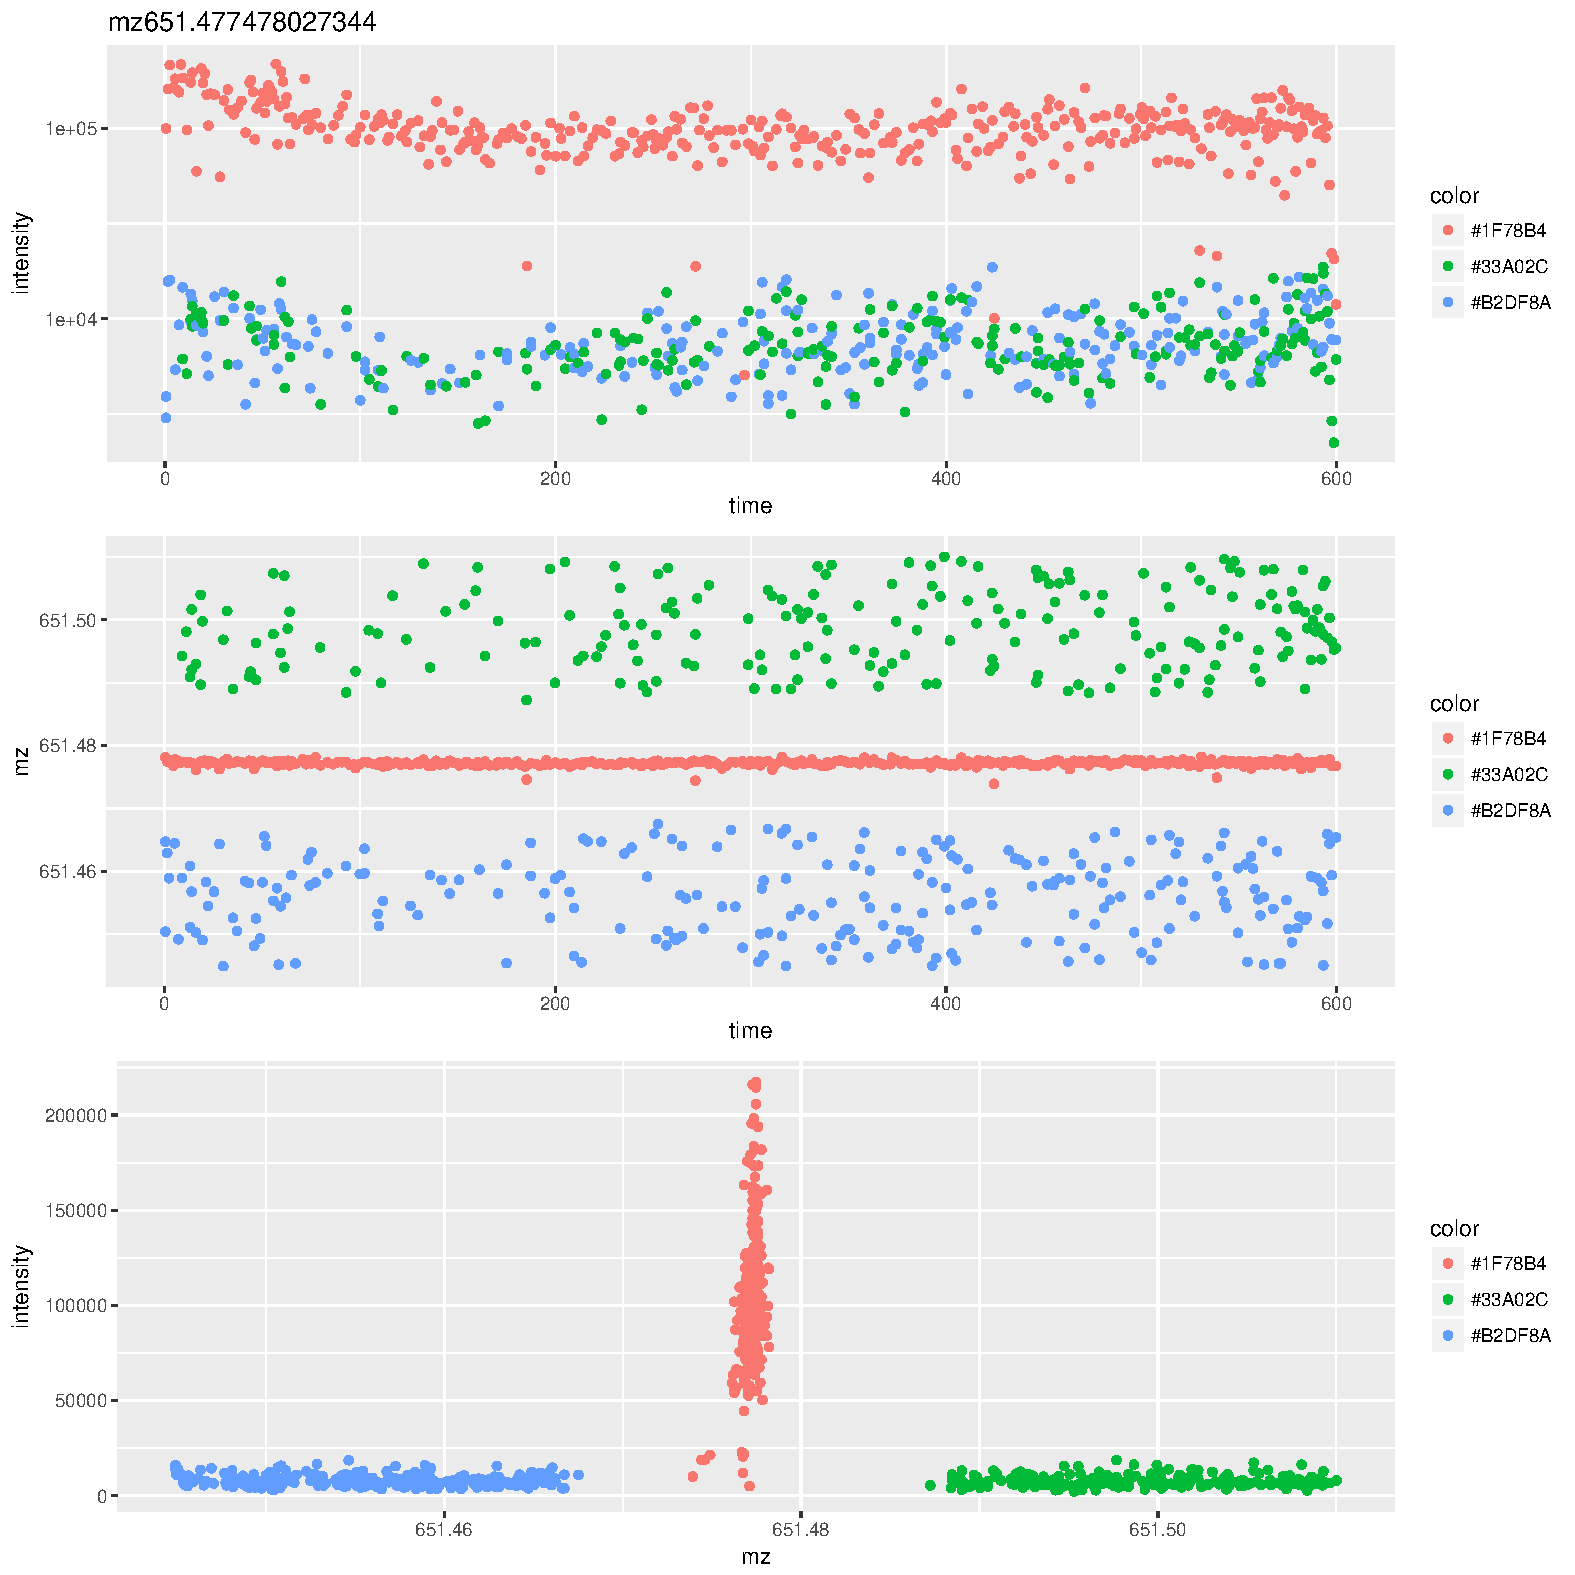
\includegraphics{Supplementary_document_files/figure-latex/cluster.mz.651-1.pdf}
NULL

\begin{Shaded}
\begin{Highlighting}[]
\NormalTok{  l<-}\KeywordTok{lm}\NormalTok{(mz }\OperatorTok{~}\StringTok{ }\NormalTok{time, }\DataTypeTok{data =}\NormalTok{ p[id.}\DecValTok{1}\NormalTok{, ])}
\ControlFlowTok{if}\NormalTok{ (}\KeywordTok{all}\NormalTok{(}\OperatorTok{!}\KeywordTok{is.na}\NormalTok{(l}\OperatorTok{$}\NormalTok{coefficients))) \{}
\NormalTok{  op <-}\StringTok{ }\KeywordTok{par}\NormalTok{(}\DataTypeTok{mfrow =} \KeywordTok{c}\NormalTok{(}\DecValTok{2}\NormalTok{, }\DecValTok{2}\NormalTok{), }\DataTypeTok{oma =} \KeywordTok{c}\NormalTok{(}\DecValTok{0}\NormalTok{, }\DecValTok{0}\NormalTok{, }\DecValTok{2}\NormalTok{, }\DecValTok{0}\NormalTok{))}
  \KeywordTok{plot}\NormalTok{(l)}
  \KeywordTok{par}\NormalTok{(op)}
\NormalTok{\}}
\end{Highlighting}
\end{Shaded}

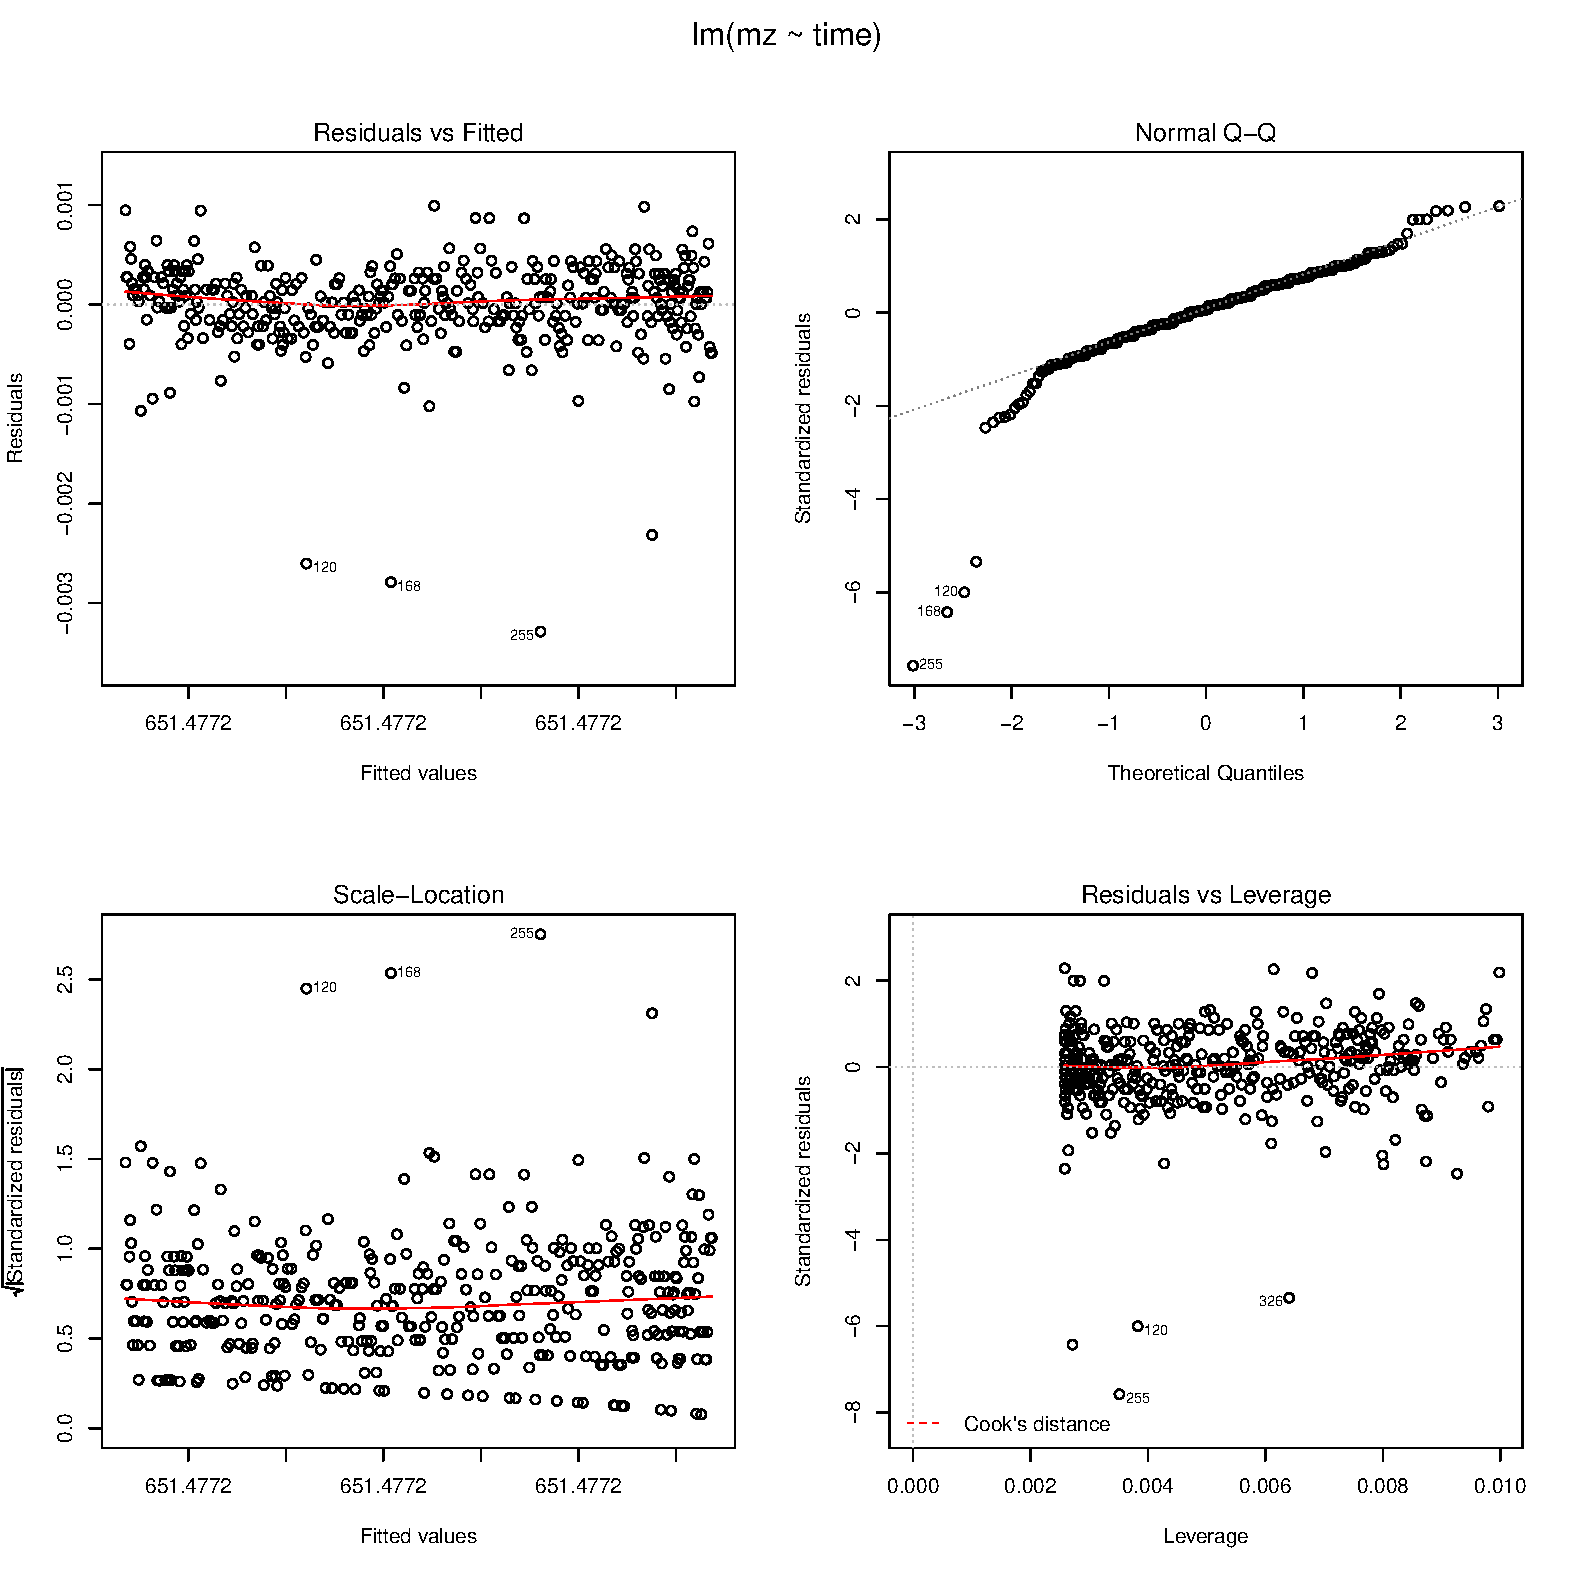
\includegraphics{Supplementary_document_files/figure-latex/fit.lin.651-1.pdf}

\begin{Shaded}
\begin{Highlighting}[]
\ControlFlowTok{if}\NormalTok{ (}\KeywordTok{all}\NormalTok{(}\OperatorTok{!}\KeywordTok{is.na}\NormalTok{(l}\OperatorTok{$}\NormalTok{coefficients))) \{}
  \KeywordTok{range}\NormalTok{(l}\OperatorTok{$}\NormalTok{residuals[}\KeywordTok{abs}\NormalTok{(}\KeywordTok{rstandard}\NormalTok{(l)) }\OperatorTok{<=}\StringTok{ }\DecValTok{2}\NormalTok{]) ->}\StringTok{ }\NormalTok{bnd}
\NormalTok{  pl <-}\StringTok{ }\KeywordTok{predict}\NormalTok{(l, p.)}
\NormalTok{  rl <-}\StringTok{ }\NormalTok{p.}\OperatorTok{$}\NormalTok{mz }\OperatorTok{-}\StringTok{ }\NormalTok{pl}
\NormalTok{  idL <-}\StringTok{ }\KeywordTok{which}\NormalTok{(rl }\OperatorTok{>=}\StringTok{ }\NormalTok{bnd[}\DecValTok{1}\NormalTok{] }\OperatorTok{&}\StringTok{ }\NormalTok{rl }\OperatorTok{<=}\StringTok{ }\NormalTok{bnd[}\DecValTok{2}\NormalTok{])}
\NormalTok{  p5 =}\StringTok{ }\KeywordTok{qplot}\NormalTok{(}
\NormalTok{          time,}
\NormalTok{          mz,}
          \DataTypeTok{data =}\NormalTok{ p.[idL],}
          \DataTypeTok{color =}\NormalTok{ color,}
          \DataTypeTok{xlim =} \KeywordTok{range}\NormalTok{(p.}\OperatorTok{$}\NormalTok{time),}
          \DataTypeTok{ylim =} \KeywordTok{range}\NormalTok{(p.}\OperatorTok{$}\NormalTok{mz)}
\NormalTok{  )}
\NormalTok{  p6 =}\StringTok{ }\KeywordTok{qplot}\NormalTok{(time,}
\NormalTok{          mz,}
          \DataTypeTok{data =}\NormalTok{ p.,}
          \DataTypeTok{color =}\NormalTok{ color) }\OperatorTok{+}
\StringTok{      }\KeywordTok{geom_abline}\NormalTok{(}\DataTypeTok{intercept =}\NormalTok{ l}\OperatorTok{$}\NormalTok{coefficients[}\DecValTok{1}\NormalTok{],}
          \DataTypeTok{slope =}\NormalTok{ l}\OperatorTok{$}\NormalTok{coefficients[}\DecValTok{2}\NormalTok{])}
  
\NormalTok{  p.}\OperatorTok{$}\NormalTok{resPPM<-rl}\OperatorTok{*}\FloatTok{1e6}\OperatorTok{/}\NormalTok{l}\OperatorTok{$}\NormalTok{coefficients[}\DecValTok{1}\NormalTok{]}
\NormalTok{  p7<-}\KeywordTok{qplot}\NormalTok{(resPPM,}\DataTypeTok{data=}\NormalTok{p.[idL],}
            \DataTypeTok{binwidth=}\NormalTok{binwidth,}\DataTypeTok{color=}\NormalTok{color)}\OperatorTok{+}
\StringTok{    }\KeywordTok{stat_function}\NormalTok{(}\DataTypeTok{fun =} \ControlFlowTok{function}\NormalTok{(x, mean, sd, n, bw)\{}
      \KeywordTok{dnorm}\NormalTok{(}\DataTypeTok{x =}\NormalTok{ x, }\DataTypeTok{mean =}\NormalTok{ mean, }\DataTypeTok{sd =}\NormalTok{ sd) }\OperatorTok{*}\StringTok{ }\NormalTok{n }\OperatorTok{*}\StringTok{ }\NormalTok{bw}
\NormalTok{      \},}
      \DataTypeTok{args =} \KeywordTok{c}\NormalTok{(}\DataTypeTok{mean =} \KeywordTok{mean}\NormalTok{(p.}\OperatorTok{$}\NormalTok{resPPM[idL]), }
               \DataTypeTok{sd =} \KeywordTok{sd}\NormalTok{(p.}\OperatorTok{$}\NormalTok{resPPM[idL]), }
               \DataTypeTok{n =} \KeywordTok{length}\NormalTok{(idL), }
               \DataTypeTok{bw =}\NormalTok{ binwidth))}

  \KeywordTok{print}\NormalTok{(}\KeywordTok{multiplot}\NormalTok{(p5, p6, p7, }\DataTypeTok{cols =} \DecValTok{1}\NormalTok{))}
\NormalTok{\}}
\end{Highlighting}
\end{Shaded}

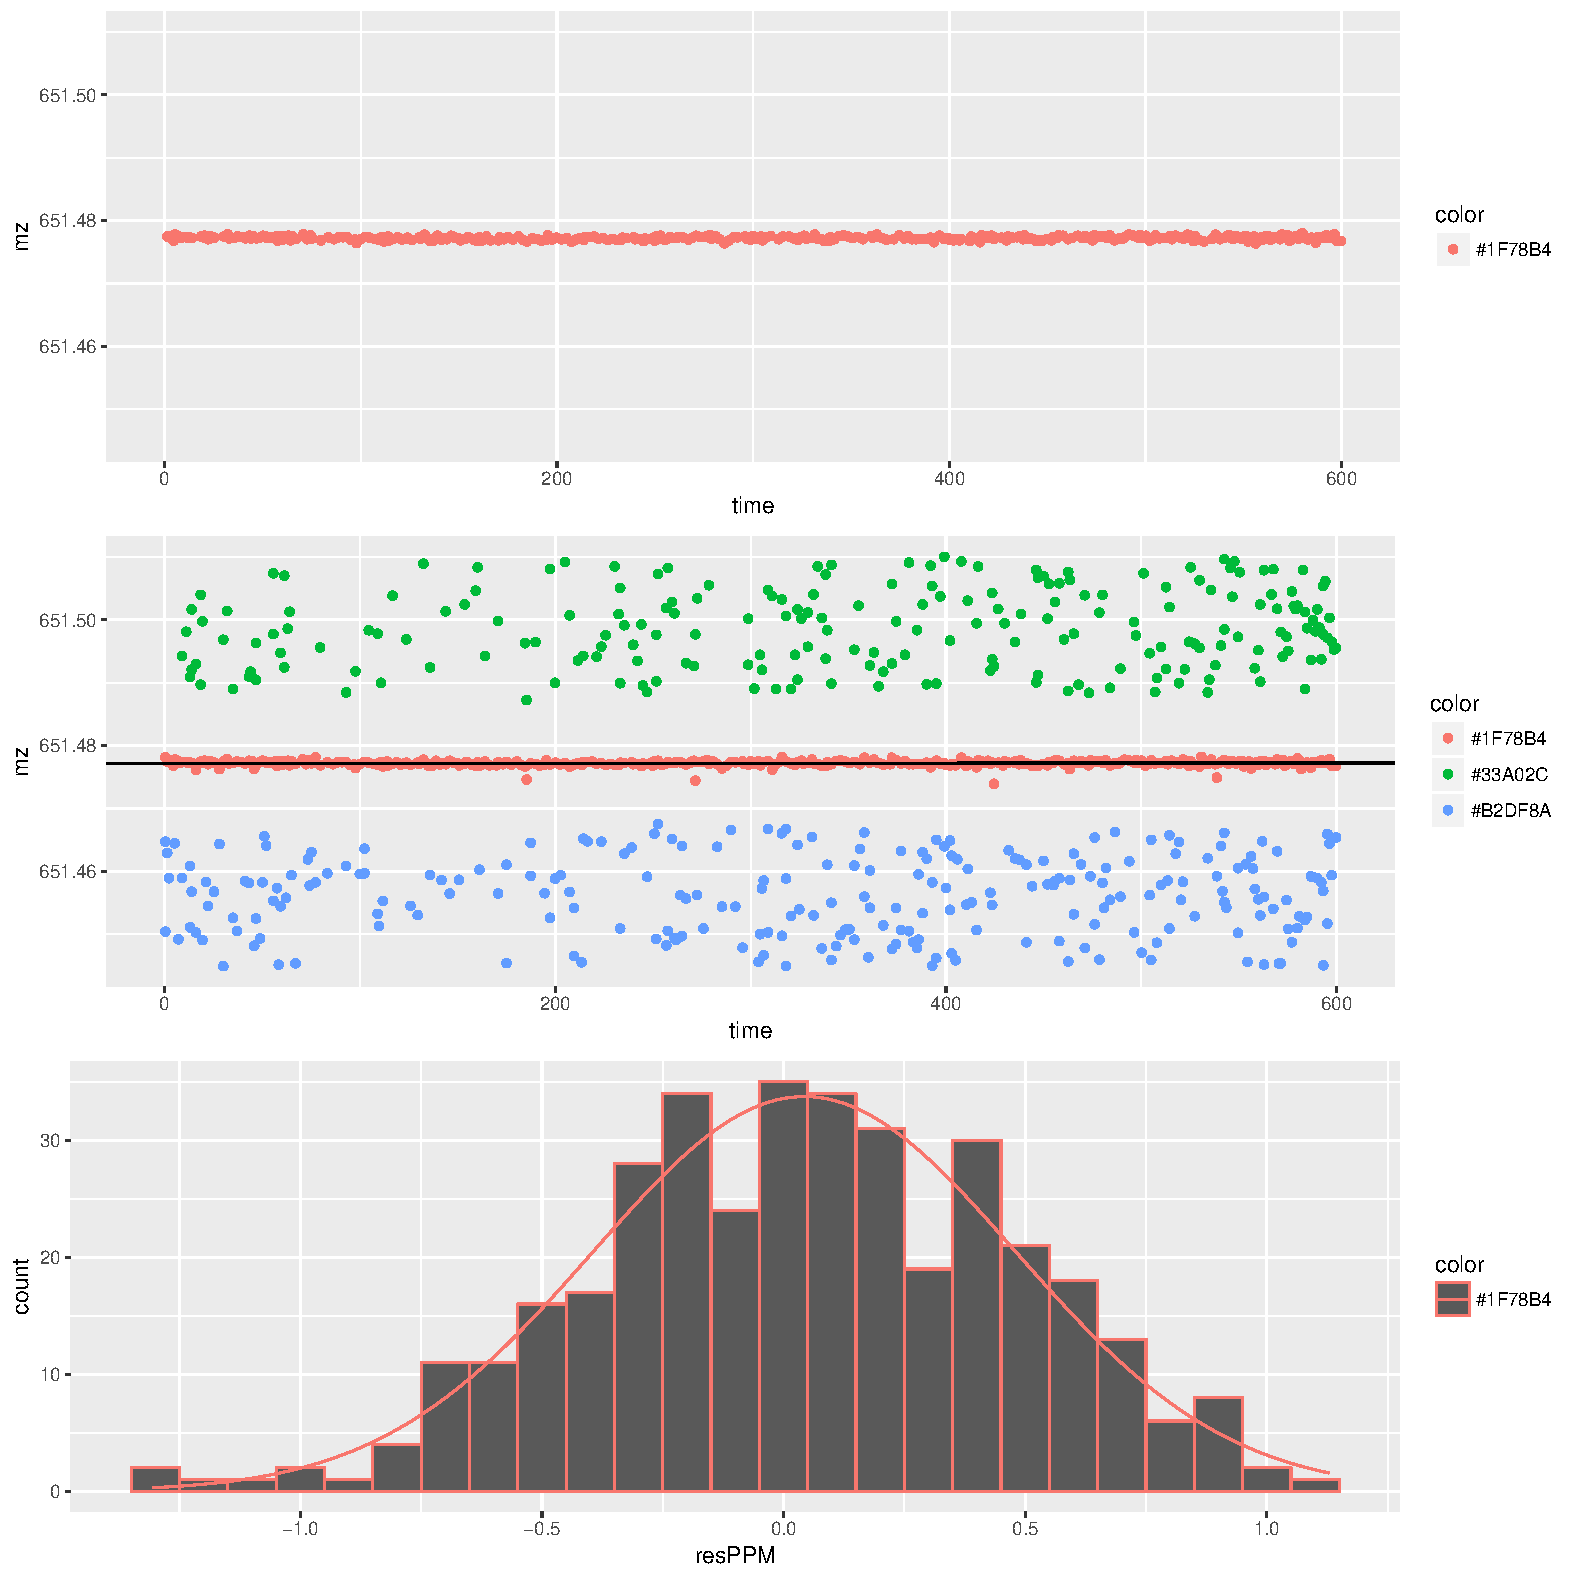
\includegraphics{Supplementary_document_files/figure-latex/filter.lm.651-1.pdf}
NULL

\section{MZ=600.513493}\label{mz600.513493}

\begin{Shaded}
\begin{Highlighting}[]
\NormalTok{  idx<-}\KeywordTok{which}\NormalTok{(}\KeywordTok{abs}\NormalTok{(p}\OperatorTok{$}\NormalTok{mz}\OperatorTok{-}\FloatTok{600.513493}\NormalTok{)}\OperatorTok{<}\FloatTok{1e-3}\NormalTok{)}
\NormalTok{  cP<-}\KeywordTok{which.max}\NormalTok{(p}\OperatorTok{$}\NormalTok{intensity[idx])}
\NormalTok{  ionI<-idx[cP]}
\NormalTok{  maxMZ<-p}\OperatorTok{$}\NormalTok{mz[ionI]}
\end{Highlighting}
\end{Shaded}

The selected row represents the peak with m/z=600.5134 of the scan N=45
taken at time 59.4 sec:

\begin{Shaded}
\begin{Highlighting}[]
\KeywordTok{print}\NormalTok{(}\KeywordTok{getScanPlot}\NormalTok{(p[scan}\OperatorTok{==}\NormalTok{p}\OperatorTok{$}\NormalTok{scan[ionI]]))}
\end{Highlighting}
\end{Shaded}

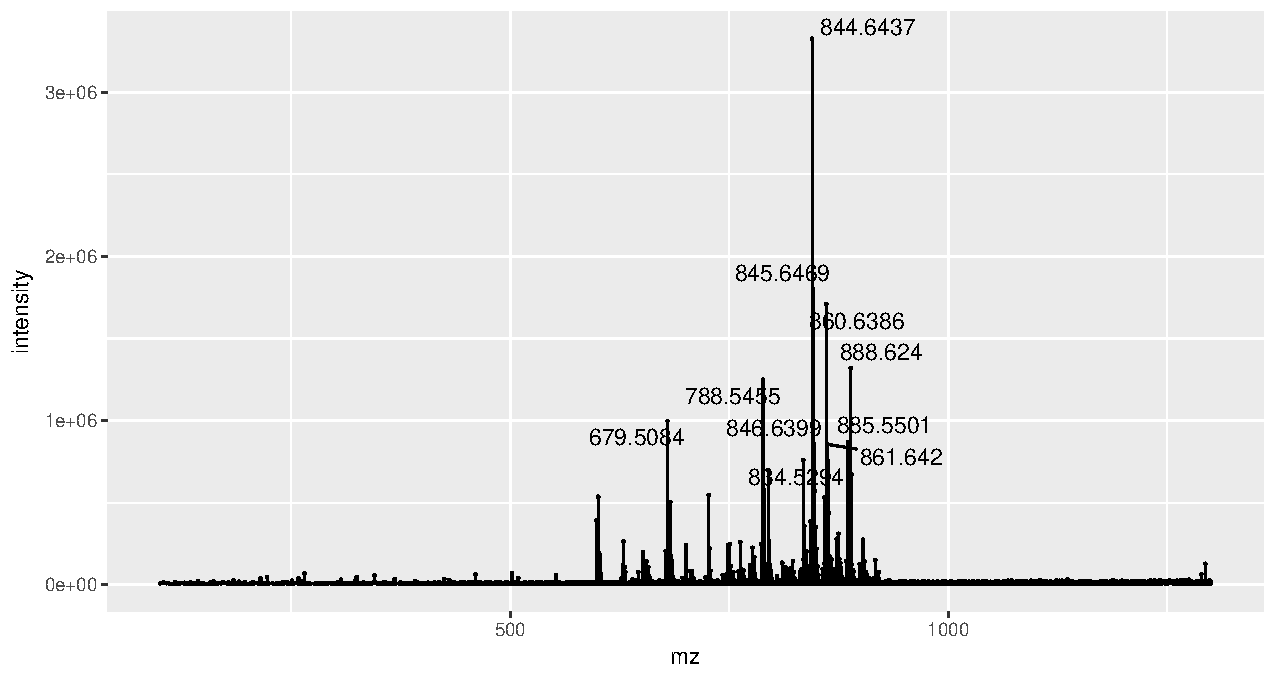
\includegraphics{Supplementary_document_files/figure-latex/ion.plots.600-1.pdf}

Now we collect all signals in the vicinity (50 ppm) of the selected m/z
value and analyze how they drift with time:

\begin{Shaded}
\begin{Highlighting}[]
\NormalTok{  idx <-}\StringTok{ }\KeywordTok{which}\NormalTok{(}\KeywordTok{abs}\NormalTok{(p}\OperatorTok{$}\NormalTok{mz }\OperatorTok{-}\StringTok{ }\NormalTok{maxMZ) }\OperatorTok{<}\StringTok{ }\NormalTok{(ppm }\OperatorTok{*}\StringTok{ }\FloatTok{1e-6} \OperatorTok{*}\StringTok{ }\NormalTok{maxMZ))}
\NormalTok{  p. <-}\StringTok{ }\NormalTok{p[idx, ]}
\end{Highlighting}
\end{Shaded}

To separate feature from surrounding noise we cluster data in m/z domain
by hierarchical Ward clustering and select the most stable clusters with
dynamicTreeCut:

\begin{Shaded}
\begin{Highlighting}[]
\NormalTok{  dissim1 =}\StringTok{ }\KeywordTok{dist}\NormalTok{(p.}\OperatorTok{$}\NormalTok{mz)}
\NormalTok{  dendro1 <-}\StringTok{ }\KeywordTok{hclust}\NormalTok{(}\DataTypeTok{d =}\NormalTok{ dissim1, }\DataTypeTok{method =} \StringTok{'ward.D2'}\NormalTok{)}
\NormalTok{  ct1 <-}\StringTok{ }\KeywordTok{cutreeDynamic}\NormalTok{(}
\NormalTok{    dendro1,}
    \DataTypeTok{cutHeight =} \OtherTok{NULL}\NormalTok{,}
    \DataTypeTok{minClusterSize =} \DecValTok{30}\NormalTok{,}
    \DataTypeTok{method =} \StringTok{"hybrid"}\NormalTok{,}
    \DataTypeTok{deepSplit =} \DecValTok{0}\NormalTok{,}
    \DataTypeTok{pamStage =} \OtherTok{TRUE}\NormalTok{,}
    \DataTypeTok{distM =} \KeywordTok{as.matrix}\NormalTok{(dissim1),}
    \DataTypeTok{maxPamDist =} \DecValTok{0}\NormalTok{,}
    \DataTypeTok{verbose =} \DecValTok{0}
\NormalTok{  )}
\NormalTok{  cct1 <-}\StringTok{ }\NormalTok{ct1[}\KeywordTok{which.max}\NormalTok{(p.}\OperatorTok{$}\NormalTok{intensity)]}
\NormalTok{  id.}\DecValTok{1}\NormalTok{ <-}\StringTok{ }\NormalTok{idx[ct1 }\OperatorTok{==}\StringTok{ }\NormalTok{cct1]}
\NormalTok{  mz1 <-}\StringTok{ }\KeywordTok{median}\NormalTok{(p}\OperatorTok{$}\NormalTok{mz[id.}\DecValTok{1}\NormalTok{])}
\NormalTok{  p.}\OperatorTok{$}\NormalTok{color<-.pal[ct1}\OperatorTok{+}\DecValTok{1}\NormalTok{]}
\NormalTok{  rl <-}\StringTok{ }\KeywordTok{get_runLen}\NormalTok{(p}\OperatorTok{$}\NormalTok{scan[id.}\DecValTok{1}\NormalTok{], scanLen)}
\NormalTok{  p1<-}\KeywordTok{qplot}\NormalTok{(time,intensity,}\DataTypeTok{data =}\NormalTok{ p.,}\DataTypeTok{main=}\KeywordTok{paste0}\NormalTok{(}\StringTok{'mz'}\NormalTok{,maxMZ),}\DataTypeTok{log=}\StringTok{'y'}\NormalTok{,}\DataTypeTok{color=}\NormalTok{color)}
\NormalTok{  p2<-}\KeywordTok{qplot}\NormalTok{(time,mz,}\DataTypeTok{data =}\NormalTok{ p.,}\DataTypeTok{color=}\NormalTok{color)}
\NormalTok{  p3<-}\KeywordTok{qplot}\NormalTok{(mz,intensity,}\DataTypeTok{data =}\NormalTok{ p.,}\DataTypeTok{color=}\NormalTok{color)}
  \KeywordTok{print}\NormalTok{(}\KeywordTok{multiplot}\NormalTok{(p1, p2, p3, }\DataTypeTok{cols=}\DecValTok{1}\NormalTok{))}
\end{Highlighting}
\end{Shaded}

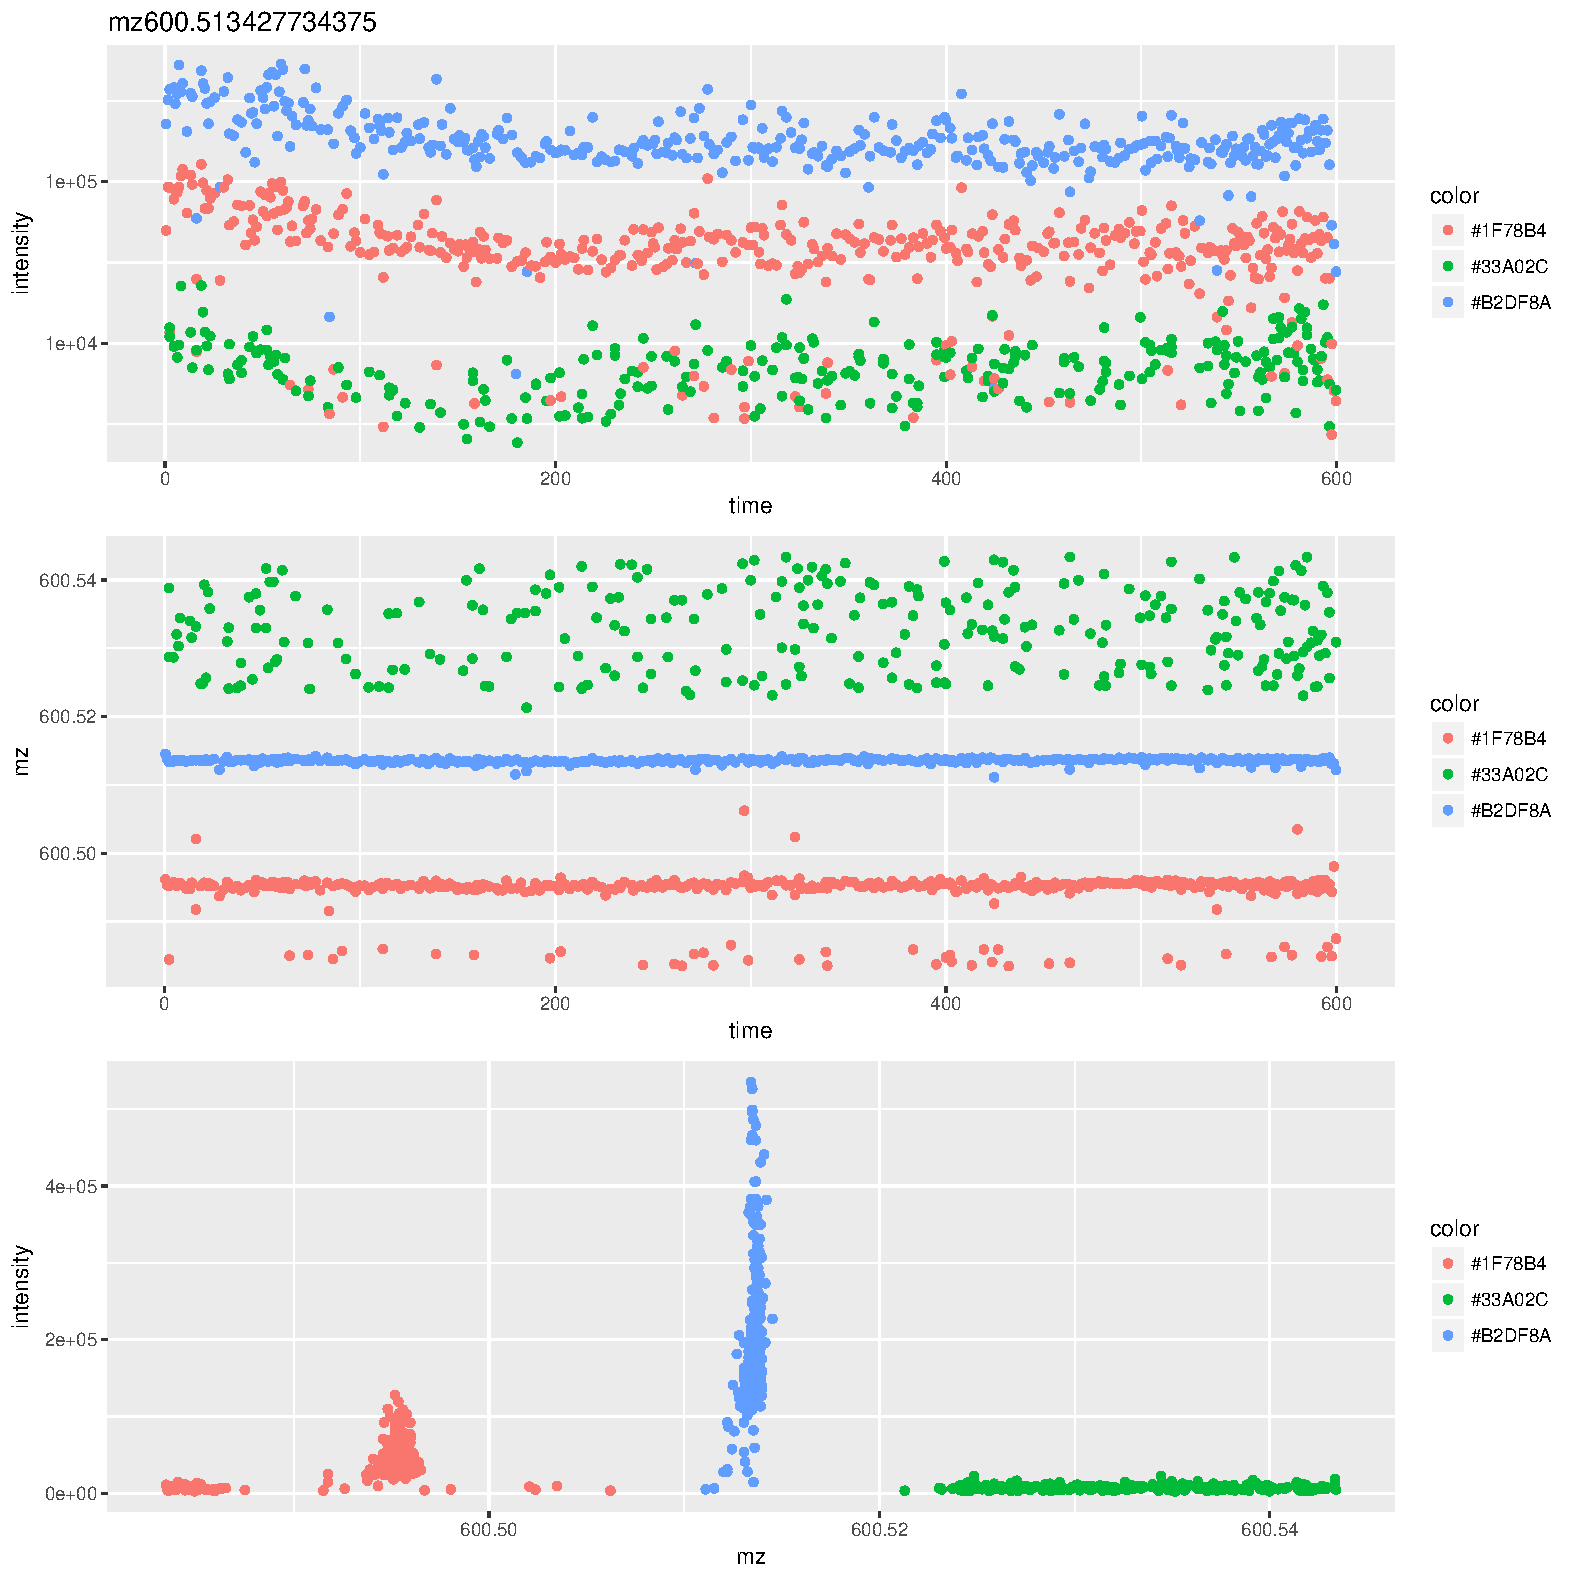
\includegraphics{Supplementary_document_files/figure-latex/cluster.mz.600-1.pdf}
NULL

\begin{Shaded}
\begin{Highlighting}[]
\NormalTok{  l<-}\KeywordTok{lm}\NormalTok{(mz }\OperatorTok{~}\StringTok{ }\NormalTok{time, }\DataTypeTok{data =}\NormalTok{ p[id.}\DecValTok{1}\NormalTok{, ])}
\ControlFlowTok{if}\NormalTok{ (}\KeywordTok{all}\NormalTok{(}\OperatorTok{!}\KeywordTok{is.na}\NormalTok{(l}\OperatorTok{$}\NormalTok{coefficients))) \{}
\NormalTok{  op <-}\StringTok{ }\KeywordTok{par}\NormalTok{(}\DataTypeTok{mfrow =} \KeywordTok{c}\NormalTok{(}\DecValTok{2}\NormalTok{, }\DecValTok{2}\NormalTok{), }\DataTypeTok{oma =} \KeywordTok{c}\NormalTok{(}\DecValTok{0}\NormalTok{, }\DecValTok{0}\NormalTok{, }\DecValTok{2}\NormalTok{, }\DecValTok{0}\NormalTok{))}
  \KeywordTok{plot}\NormalTok{(l)}
  \KeywordTok{par}\NormalTok{(op)}
\NormalTok{\}}
\end{Highlighting}
\end{Shaded}

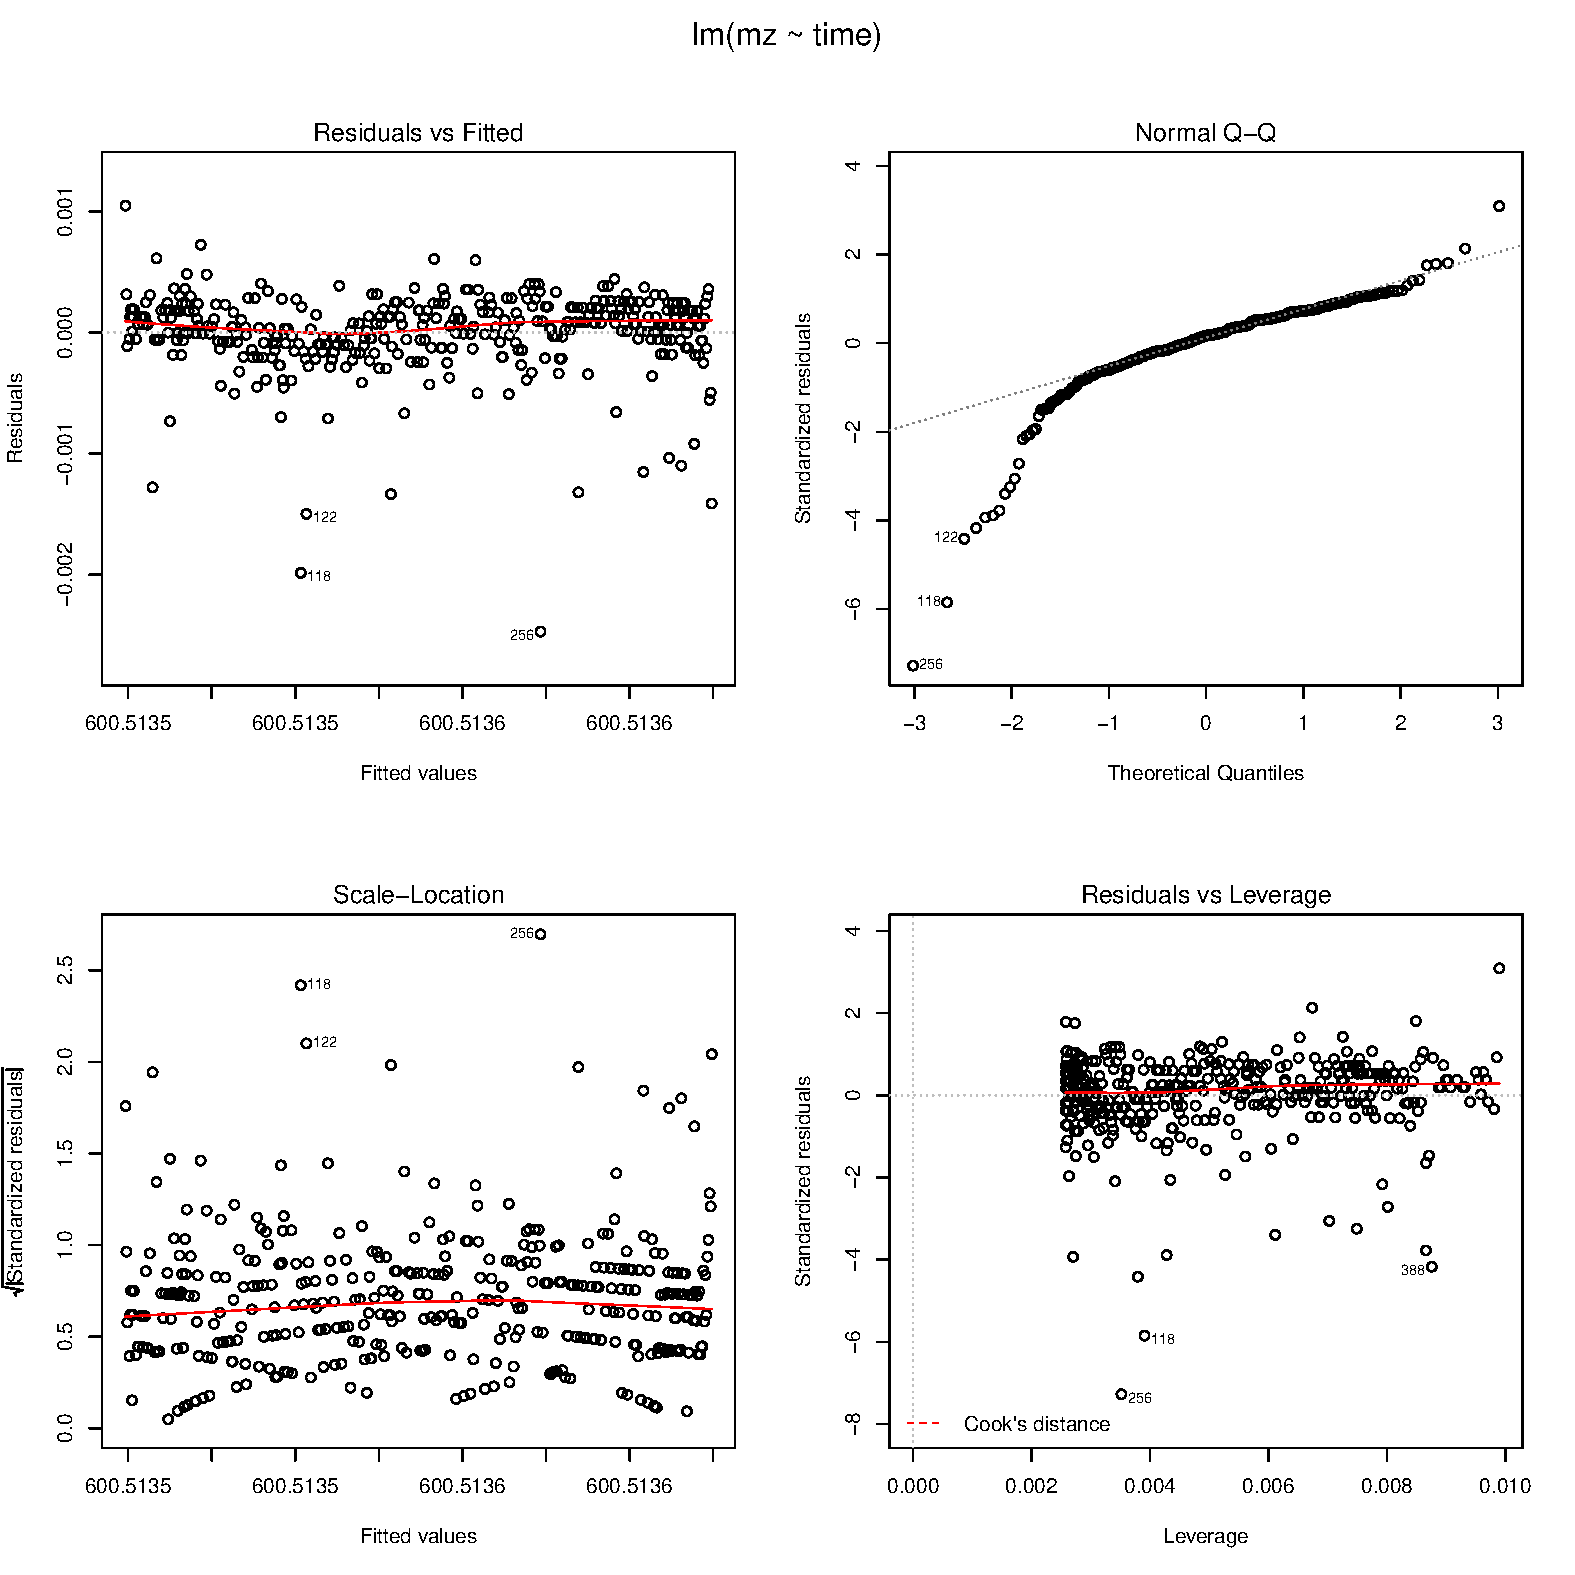
\includegraphics{Supplementary_document_files/figure-latex/fit.lin.600-1.pdf}

\begin{Shaded}
\begin{Highlighting}[]
\ControlFlowTok{if}\NormalTok{ (}\KeywordTok{all}\NormalTok{(}\OperatorTok{!}\KeywordTok{is.na}\NormalTok{(l}\OperatorTok{$}\NormalTok{coefficients))) \{}
  \KeywordTok{range}\NormalTok{(l}\OperatorTok{$}\NormalTok{residuals[}\KeywordTok{abs}\NormalTok{(}\KeywordTok{rstandard}\NormalTok{(l)) }\OperatorTok{<=}\StringTok{ }\DecValTok{2}\NormalTok{]) ->}\StringTok{ }\NormalTok{bnd}
\NormalTok{  pl <-}\StringTok{ }\KeywordTok{predict}\NormalTok{(l, p.)}
\NormalTok{  rl <-}\StringTok{ }\NormalTok{p.}\OperatorTok{$}\NormalTok{mz }\OperatorTok{-}\StringTok{ }\NormalTok{pl}
\NormalTok{  idL <-}\StringTok{ }\KeywordTok{which}\NormalTok{(rl }\OperatorTok{>=}\StringTok{ }\NormalTok{bnd[}\DecValTok{1}\NormalTok{] }\OperatorTok{&}\StringTok{ }\NormalTok{rl }\OperatorTok{<=}\StringTok{ }\NormalTok{bnd[}\DecValTok{2}\NormalTok{])}
\NormalTok{  p5 =}\StringTok{ }\KeywordTok{qplot}\NormalTok{(}
\NormalTok{          time,}
\NormalTok{          mz,}
          \DataTypeTok{data =}\NormalTok{ p.[idL],}
          \DataTypeTok{color =}\NormalTok{ color,}
          \DataTypeTok{xlim =} \KeywordTok{range}\NormalTok{(p.}\OperatorTok{$}\NormalTok{time),}
          \DataTypeTok{ylim =} \KeywordTok{range}\NormalTok{(p.}\OperatorTok{$}\NormalTok{mz)}
\NormalTok{  )}
\NormalTok{  p6 =}\StringTok{ }\KeywordTok{qplot}\NormalTok{(time,}
\NormalTok{          mz,}
          \DataTypeTok{data =}\NormalTok{ p.,}
          \DataTypeTok{color =}\NormalTok{ color) }\OperatorTok{+}
\StringTok{      }\KeywordTok{geom_abline}\NormalTok{(}\DataTypeTok{intercept =}\NormalTok{ l}\OperatorTok{$}\NormalTok{coefficients[}\DecValTok{1}\NormalTok{],}
          \DataTypeTok{slope =}\NormalTok{ l}\OperatorTok{$}\NormalTok{coefficients[}\DecValTok{2}\NormalTok{])}
  
\NormalTok{  p.}\OperatorTok{$}\NormalTok{resPPM<-rl}\OperatorTok{*}\FloatTok{1e6}\OperatorTok{/}\NormalTok{l}\OperatorTok{$}\NormalTok{coefficients[}\DecValTok{1}\NormalTok{]}
\NormalTok{  p7<-}\KeywordTok{qplot}\NormalTok{(resPPM,}\DataTypeTok{data=}\NormalTok{p.[idL],}
            \DataTypeTok{binwidth=}\NormalTok{binwidth,}\DataTypeTok{color=}\NormalTok{color)}\OperatorTok{+}
\StringTok{    }\KeywordTok{stat_function}\NormalTok{(}\DataTypeTok{fun =} \ControlFlowTok{function}\NormalTok{(x, mean, sd, n, bw)\{}
      \KeywordTok{dnorm}\NormalTok{(}\DataTypeTok{x =}\NormalTok{ x, }\DataTypeTok{mean =}\NormalTok{ mean, }\DataTypeTok{sd =}\NormalTok{ sd) }\OperatorTok{*}\StringTok{ }\NormalTok{n }\OperatorTok{*}\StringTok{ }\NormalTok{bw}
\NormalTok{      \},}
      \DataTypeTok{args =} \KeywordTok{c}\NormalTok{(}\DataTypeTok{mean =} \KeywordTok{mean}\NormalTok{(p.}\OperatorTok{$}\NormalTok{resPPM[idL]), }
               \DataTypeTok{sd =} \KeywordTok{sd}\NormalTok{(p.}\OperatorTok{$}\NormalTok{resPPM[idL]), }
               \DataTypeTok{n =} \KeywordTok{length}\NormalTok{(idL), }
               \DataTypeTok{bw =}\NormalTok{ binwidth))}
  \KeywordTok{print}\NormalTok{(}\KeywordTok{multiplot}\NormalTok{(p5, p6, p7, }\DataTypeTok{cols =} \DecValTok{1}\NormalTok{))}
\NormalTok{\}}
\end{Highlighting}
\end{Shaded}

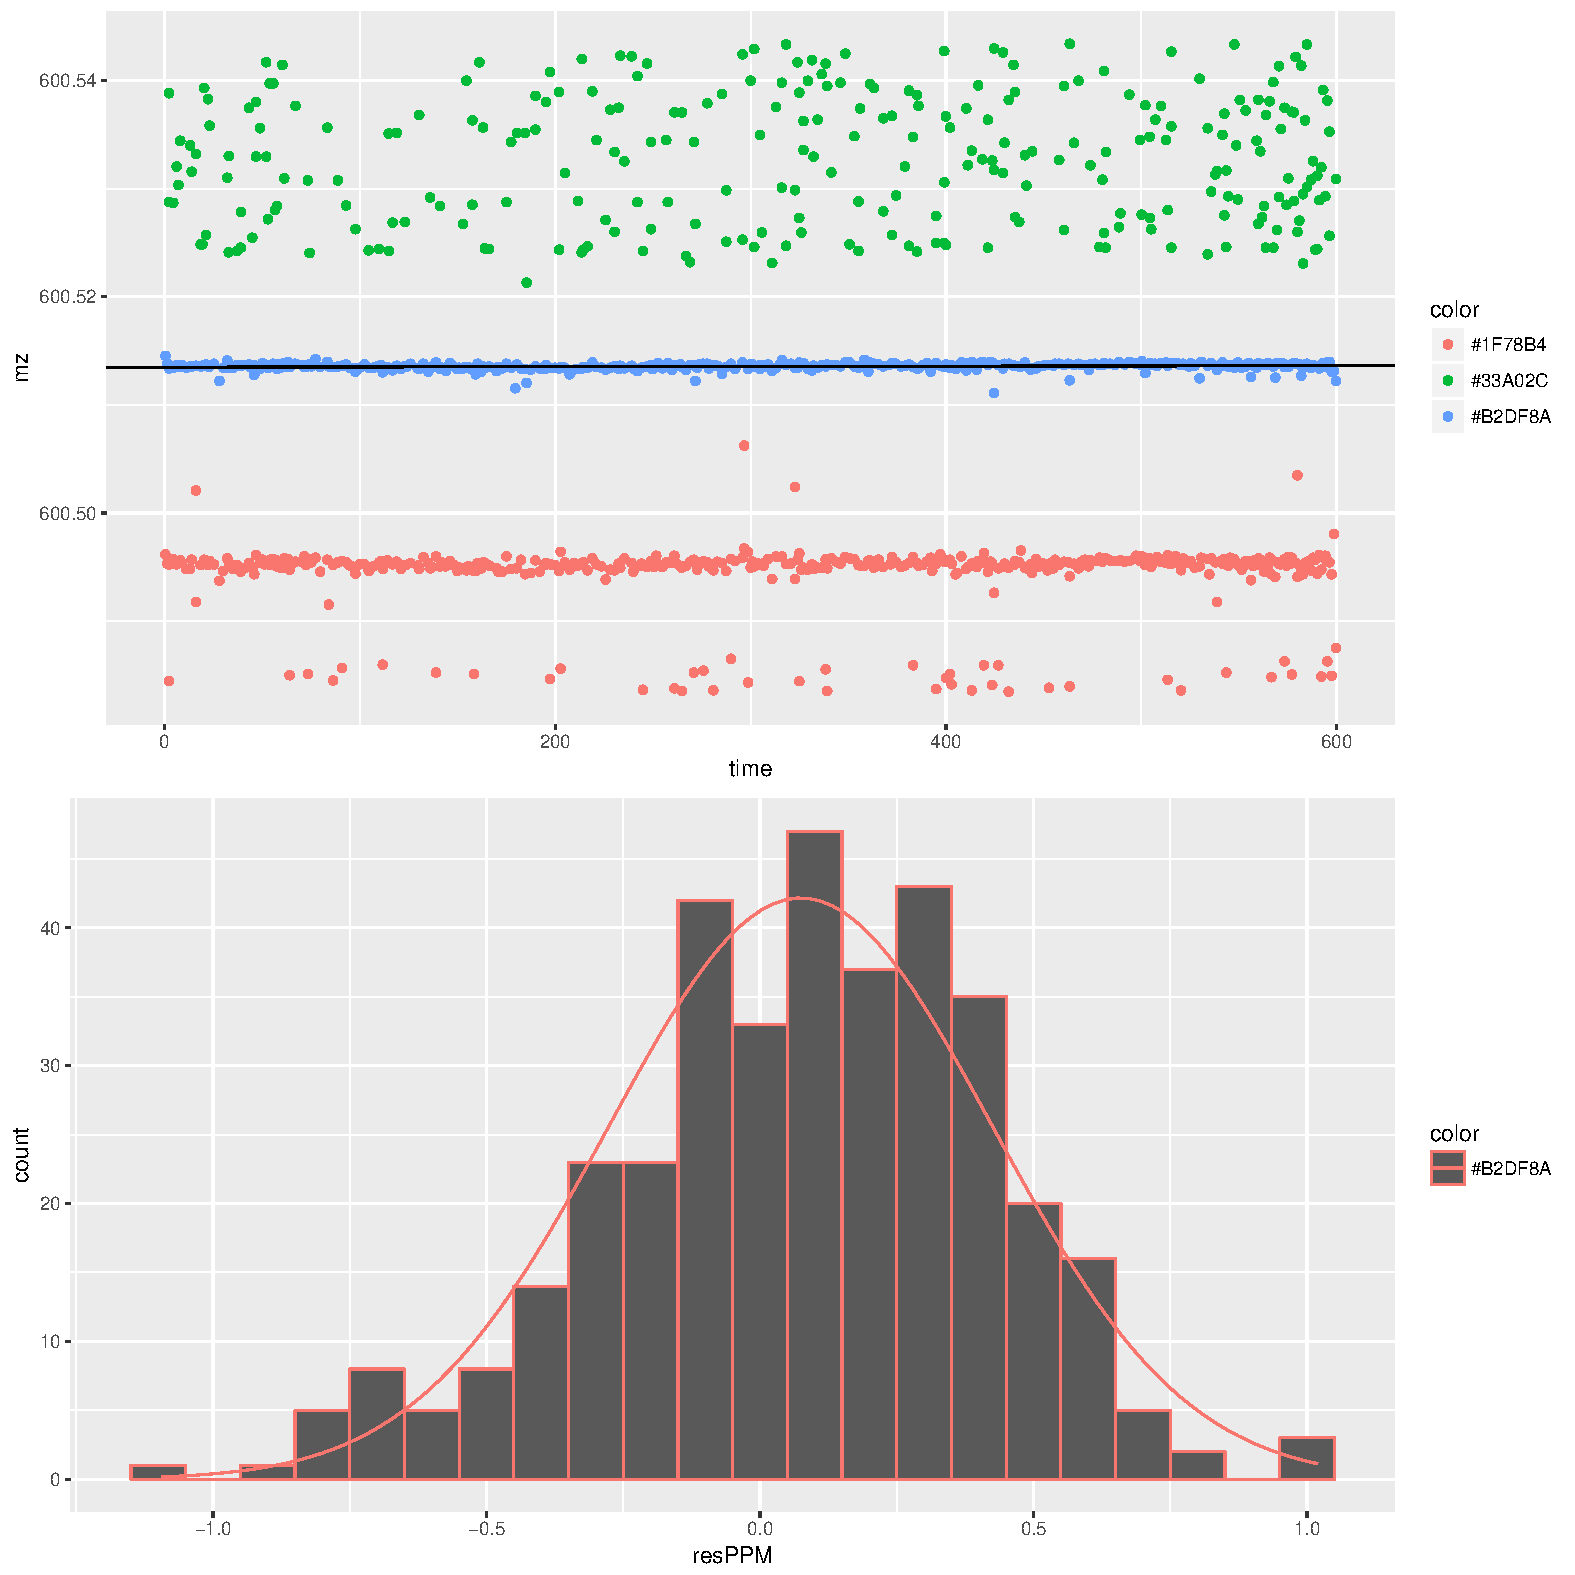
\includegraphics{Supplementary_document_files/figure-latex/filter.lm.600-1.pdf}
NULL

\section{MZ=602.510830}\label{mz602.510830}

\begin{Shaded}
\begin{Highlighting}[]
\NormalTok{  idx<-}\KeywordTok{which}\NormalTok{(}\KeywordTok{abs}\NormalTok{(p}\OperatorTok{$}\NormalTok{mz}\OperatorTok{-}\FloatTok{602.510830}\NormalTok{)}\OperatorTok{<}\FloatTok{1e-3}\NormalTok{)}
\NormalTok{  cP<-}\KeywordTok{which.max}\NormalTok{(p}\OperatorTok{$}\NormalTok{intensity[idx])}
\NormalTok{  ionI<-idx[cP]}
\NormalTok{  maxMZ<-p}\OperatorTok{$}\NormalTok{mz[ionI]}
\end{Highlighting}
\end{Shaded}

The selected row represents the peak with m/z=602.511 of the scan N=45
taken at time 59.4 sec:

\begin{Shaded}
\begin{Highlighting}[]
\KeywordTok{print}\NormalTok{(}\KeywordTok{getScanPlot}\NormalTok{(p[scan}\OperatorTok{==}\NormalTok{p}\OperatorTok{$}\NormalTok{scan[ionI]]))}
\end{Highlighting}
\end{Shaded}

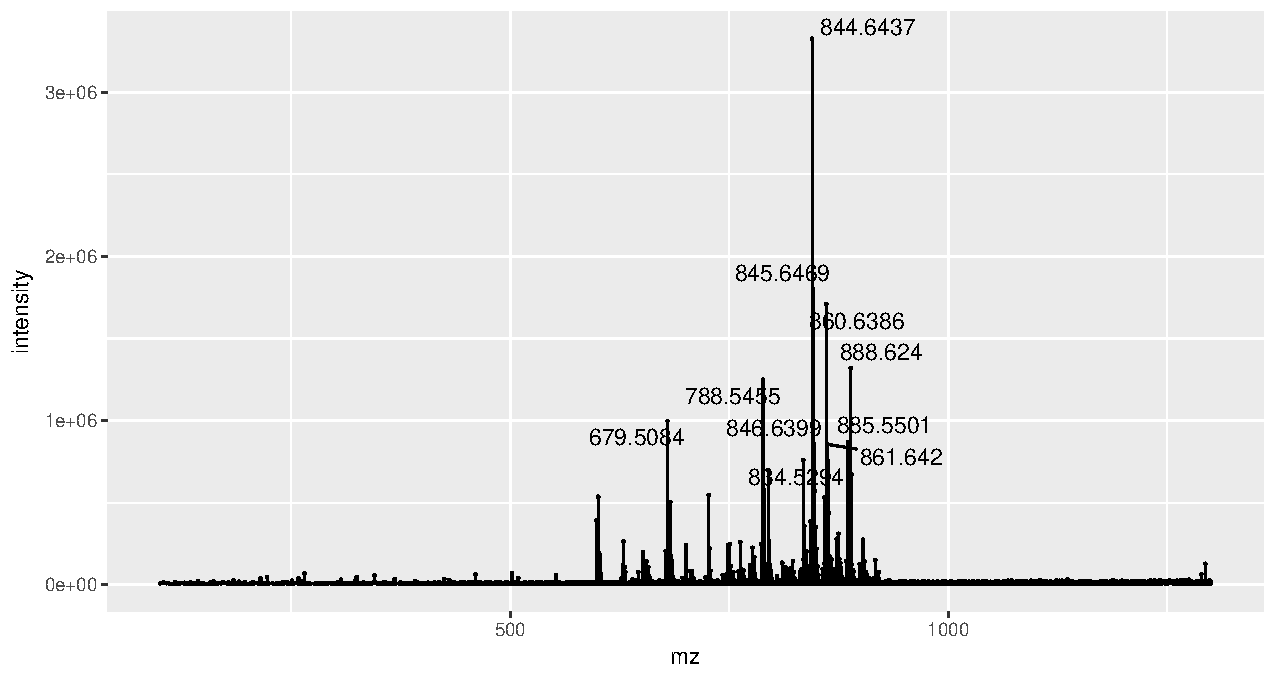
\includegraphics{Supplementary_document_files/figure-latex/ion.plots.602-1.pdf}

Now we collect all signals in the vicinity (50 ppm) of the selected m/z
value and analyze how they drift with time:

\begin{Shaded}
\begin{Highlighting}[]
\NormalTok{  idx <-}\StringTok{ }\KeywordTok{which}\NormalTok{(}\KeywordTok{abs}\NormalTok{(p}\OperatorTok{$}\NormalTok{mz }\OperatorTok{-}\StringTok{ }\NormalTok{maxMZ) }\OperatorTok{<}\StringTok{ }\NormalTok{(ppm }\OperatorTok{*}\StringTok{ }\FloatTok{1e-6} \OperatorTok{*}\StringTok{ }\NormalTok{maxMZ))}
\NormalTok{  p. <-}\StringTok{ }\NormalTok{p[idx, ]}
\end{Highlighting}
\end{Shaded}

To separate feature from surrounding noise we cluster data in m/z domain
by hierarchical Ward clustering and select the most stable clusters with
dynamicTreeCut:

\begin{Shaded}
\begin{Highlighting}[]
\NormalTok{  dissim1 =}\StringTok{ }\KeywordTok{dist}\NormalTok{(p.}\OperatorTok{$}\NormalTok{mz)}
\NormalTok{  dendro1 <-}\StringTok{ }\KeywordTok{hclust}\NormalTok{(}\DataTypeTok{d =}\NormalTok{ dissim1, }\DataTypeTok{method =} \StringTok{'ward.D2'}\NormalTok{)}
\NormalTok{  ct1 <-}\StringTok{ }\KeywordTok{cutreeDynamic}\NormalTok{(}
\NormalTok{    dendro1,}
    \DataTypeTok{cutHeight =} \OtherTok{NULL}\NormalTok{,}
    \DataTypeTok{minClusterSize =} \DecValTok{30}\NormalTok{,}
    \DataTypeTok{method =} \StringTok{"hybrid"}\NormalTok{,}
    \DataTypeTok{deepSplit =} \DecValTok{0}\NormalTok{,}
    \DataTypeTok{pamStage =} \OtherTok{TRUE}\NormalTok{,}
    \DataTypeTok{distM =} \KeywordTok{as.matrix}\NormalTok{(dissim1),}
    \DataTypeTok{maxPamDist =} \DecValTok{0}\NormalTok{,}
    \DataTypeTok{verbose =} \DecValTok{0}
\NormalTok{  )}
\NormalTok{  cct1 <-}\StringTok{ }\NormalTok{ct1[}\KeywordTok{which.max}\NormalTok{(p.}\OperatorTok{$}\NormalTok{intensity)]}
\NormalTok{  id.}\DecValTok{1}\NormalTok{ <-}\StringTok{ }\NormalTok{idx[ct1 }\OperatorTok{==}\StringTok{ }\NormalTok{cct1]}
\NormalTok{  mz1 <-}\StringTok{ }\KeywordTok{median}\NormalTok{(p}\OperatorTok{$}\NormalTok{mz[id.}\DecValTok{1}\NormalTok{])}
\NormalTok{  p.}\OperatorTok{$}\NormalTok{color<-.pal[ct1}\OperatorTok{+}\DecValTok{1}\NormalTok{]}
\NormalTok{  rl <-}\StringTok{ }\KeywordTok{get_runLen}\NormalTok{(p}\OperatorTok{$}\NormalTok{scan[id.}\DecValTok{1}\NormalTok{], scanLen)}
\NormalTok{  p1<-}\KeywordTok{qplot}\NormalTok{(time,intensity,}\DataTypeTok{data =}\NormalTok{ p.,}\DataTypeTok{main=}\KeywordTok{paste0}\NormalTok{(}\StringTok{'mz'}\NormalTok{,maxMZ),}\DataTypeTok{log=}\StringTok{'y'}\NormalTok{,}\DataTypeTok{color=}\NormalTok{color)}
\NormalTok{  p2<-}\KeywordTok{qplot}\NormalTok{(time,mz,}\DataTypeTok{data =}\NormalTok{ p.,}\DataTypeTok{color=}\NormalTok{color)}
\NormalTok{  p3<-}\KeywordTok{qplot}\NormalTok{(mz,intensity,}\DataTypeTok{data =}\NormalTok{ p.,}\DataTypeTok{color=}\NormalTok{color)}
  \KeywordTok{print}\NormalTok{(}\KeywordTok{multiplot}\NormalTok{(p1, p2, p3, }\DataTypeTok{cols=}\DecValTok{1}\NormalTok{))}
\end{Highlighting}
\end{Shaded}

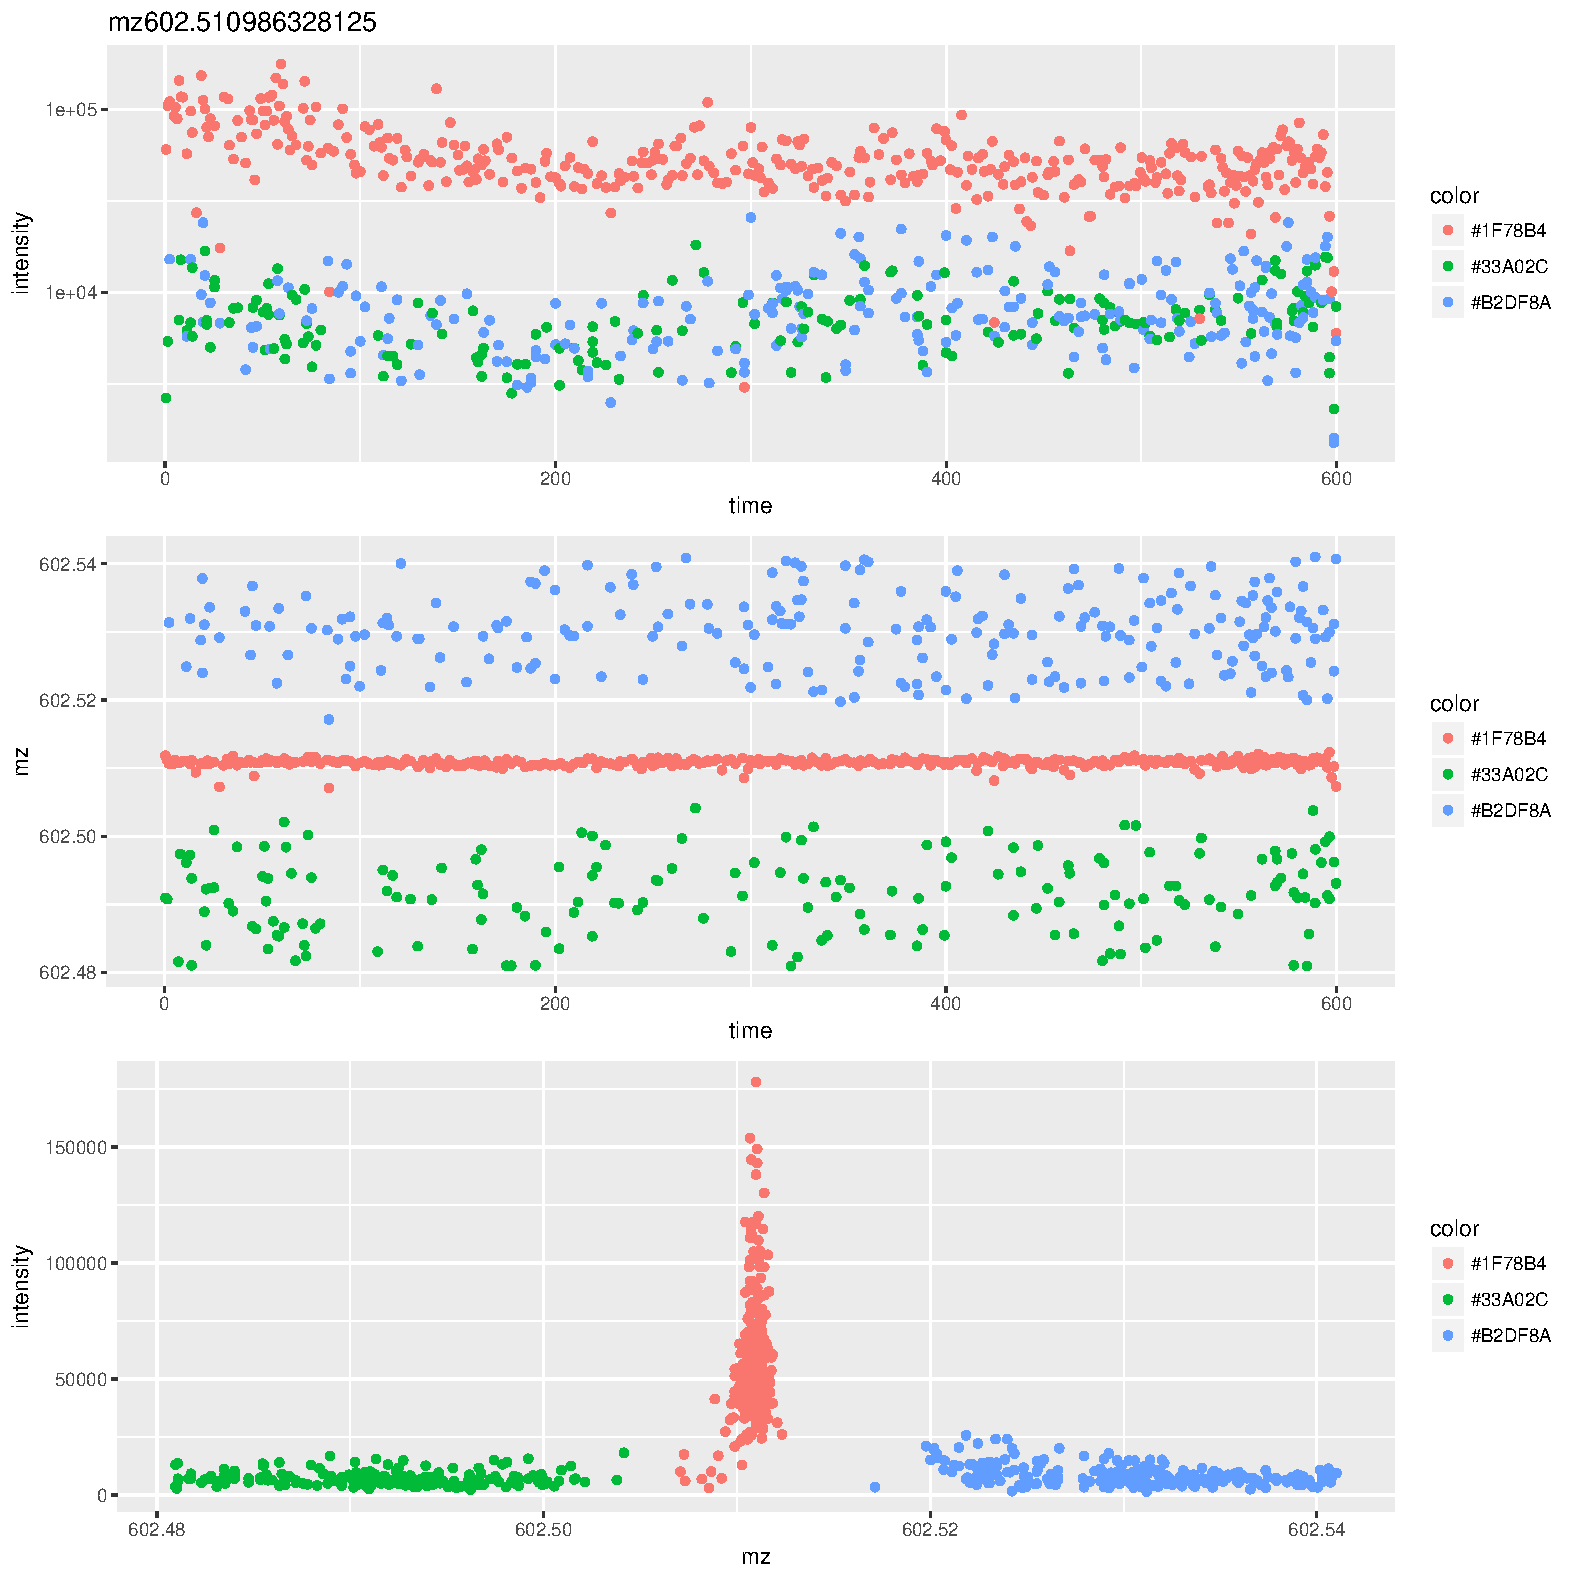
\includegraphics{Supplementary_document_files/figure-latex/cluster.mz.602-1.pdf}
NULL

\begin{Shaded}
\begin{Highlighting}[]
\NormalTok{  l<-}\KeywordTok{lm}\NormalTok{(mz }\OperatorTok{~}\StringTok{ }\NormalTok{time, }\DataTypeTok{data =}\NormalTok{ p[id.}\DecValTok{1}\NormalTok{, ])}
\ControlFlowTok{if}\NormalTok{ (}\KeywordTok{all}\NormalTok{(}\OperatorTok{!}\KeywordTok{is.na}\NormalTok{(l}\OperatorTok{$}\NormalTok{coefficients))) \{}
\NormalTok{  op <-}\StringTok{ }\KeywordTok{par}\NormalTok{(}\DataTypeTok{mfrow =} \KeywordTok{c}\NormalTok{(}\DecValTok{2}\NormalTok{, }\DecValTok{2}\NormalTok{), }\DataTypeTok{oma =} \KeywordTok{c}\NormalTok{(}\DecValTok{0}\NormalTok{, }\DecValTok{0}\NormalTok{, }\DecValTok{2}\NormalTok{, }\DecValTok{0}\NormalTok{))}
  \KeywordTok{plot}\NormalTok{(l)}
  \KeywordTok{par}\NormalTok{(op)}
\NormalTok{\}}
\end{Highlighting}
\end{Shaded}

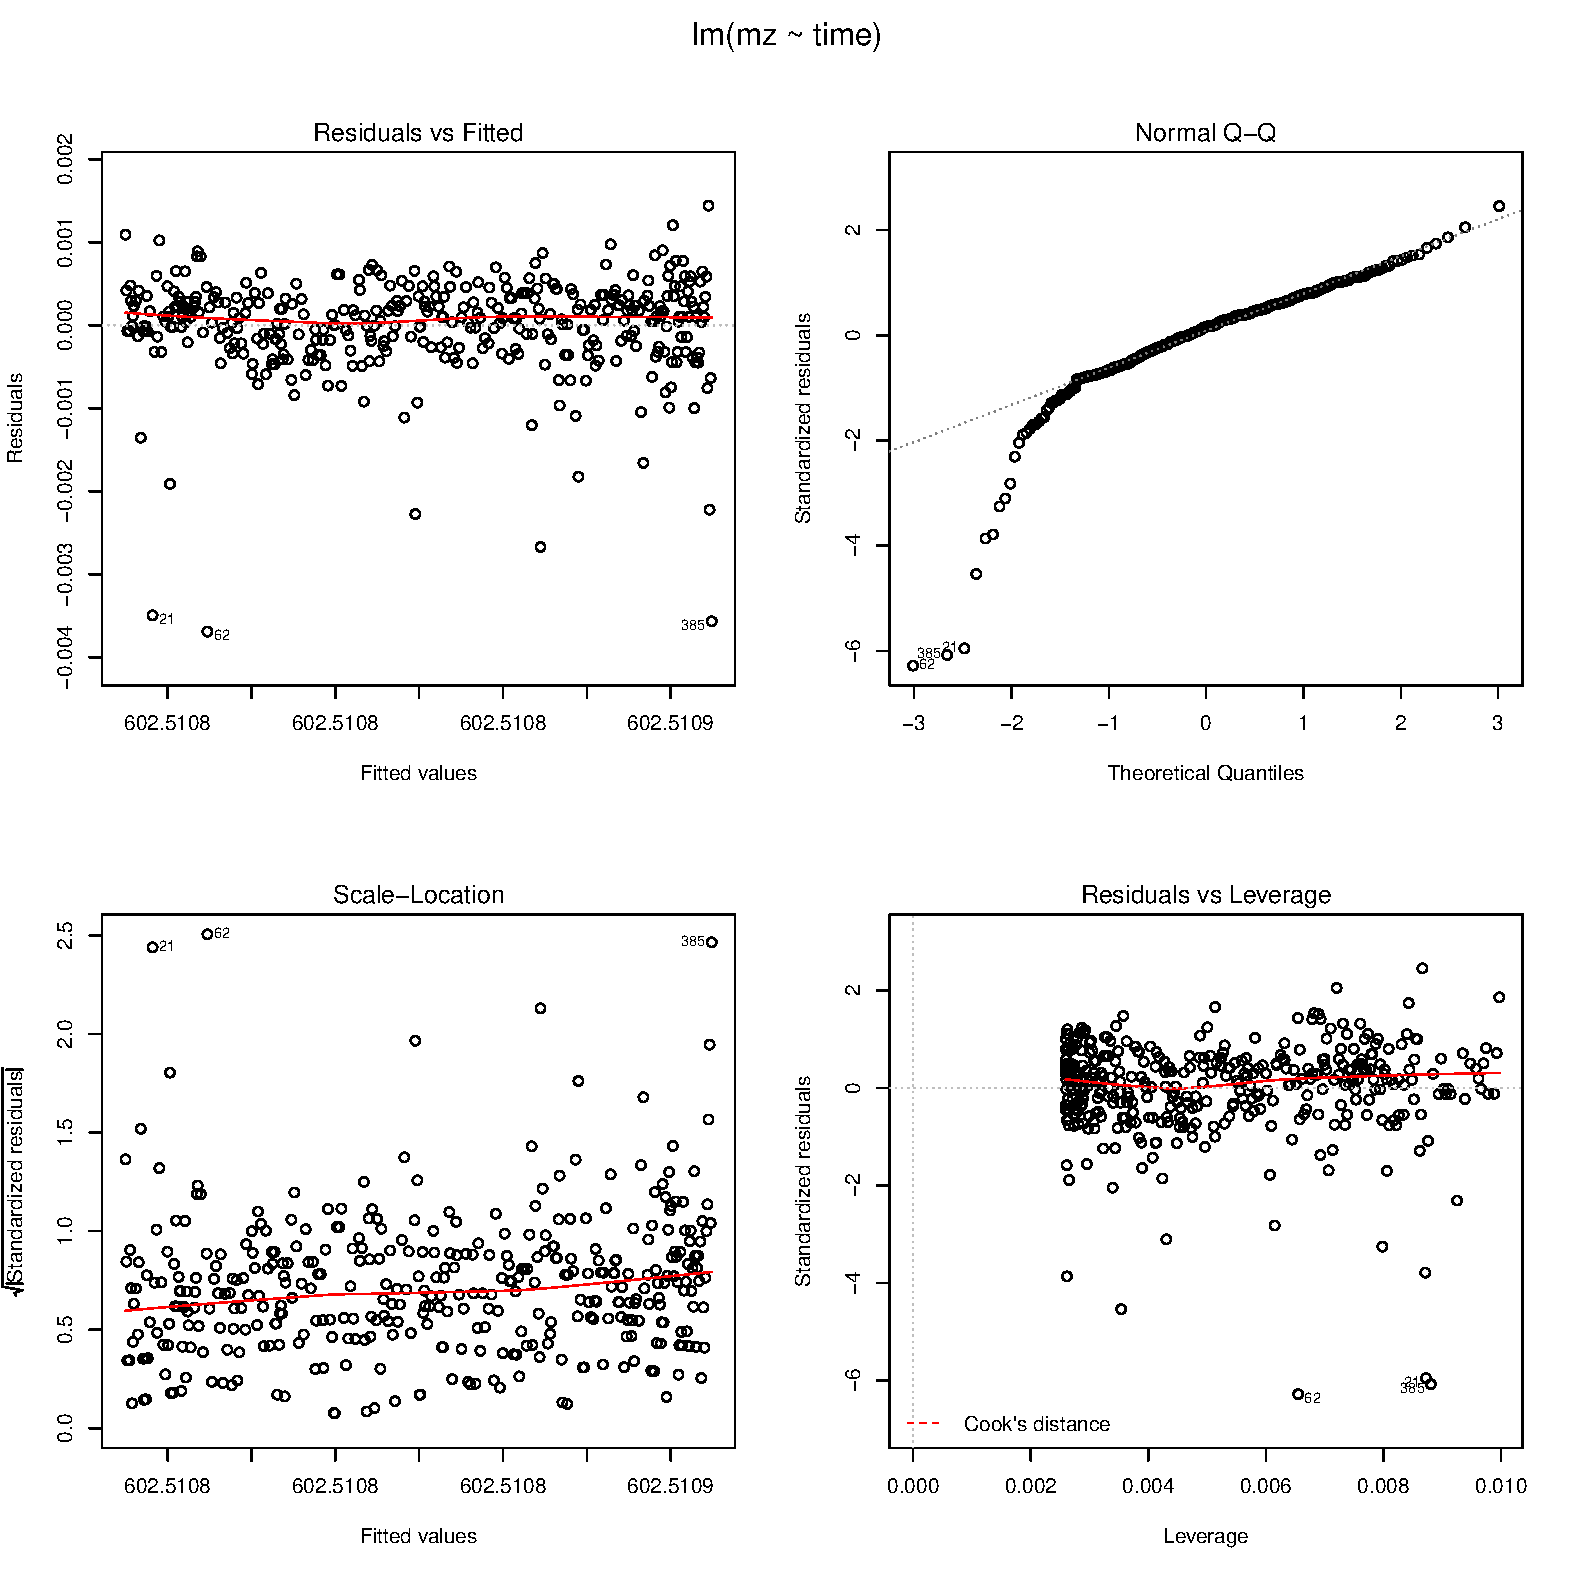
\includegraphics{Supplementary_document_files/figure-latex/fit.lin.602-1.pdf}

\begin{Shaded}
\begin{Highlighting}[]
\ControlFlowTok{if}\NormalTok{ (}\KeywordTok{all}\NormalTok{(}\OperatorTok{!}\KeywordTok{is.na}\NormalTok{(l}\OperatorTok{$}\NormalTok{coefficients))) \{}
  \KeywordTok{range}\NormalTok{(l}\OperatorTok{$}\NormalTok{residuals[}\KeywordTok{abs}\NormalTok{(}\KeywordTok{rstandard}\NormalTok{(l)) }\OperatorTok{<=}\StringTok{ }\DecValTok{2}\NormalTok{]) ->}\StringTok{ }\NormalTok{bnd}
\NormalTok{  pl <-}\StringTok{ }\KeywordTok{predict}\NormalTok{(l, p.)}
\NormalTok{  rl <-}\StringTok{ }\NormalTok{p.}\OperatorTok{$}\NormalTok{mz }\OperatorTok{-}\StringTok{ }\NormalTok{pl}
\NormalTok{  idL <-}\StringTok{ }\KeywordTok{which}\NormalTok{(rl }\OperatorTok{>=}\StringTok{ }\NormalTok{bnd[}\DecValTok{1}\NormalTok{] }\OperatorTok{&}\StringTok{ }\NormalTok{rl }\OperatorTok{<=}\StringTok{ }\NormalTok{bnd[}\DecValTok{2}\NormalTok{])}
\NormalTok{  p5 =}\StringTok{ }\KeywordTok{qplot}\NormalTok{(}
\NormalTok{          time,}
\NormalTok{          mz,}
          \DataTypeTok{data =}\NormalTok{ p.[idL],}
          \DataTypeTok{color =}\NormalTok{ color,}
          \DataTypeTok{xlim =} \KeywordTok{range}\NormalTok{(p.}\OperatorTok{$}\NormalTok{time),}
          \DataTypeTok{ylim =} \KeywordTok{range}\NormalTok{(p.}\OperatorTok{$}\NormalTok{mz)}
\NormalTok{  )}
\NormalTok{  p6 =}\StringTok{ }\KeywordTok{qplot}\NormalTok{(time,}
\NormalTok{          mz,}
          \DataTypeTok{data =}\NormalTok{ p.,}
          \DataTypeTok{color =}\NormalTok{ color) }\OperatorTok{+}
\StringTok{      }\KeywordTok{geom_abline}\NormalTok{(}\DataTypeTok{intercept =}\NormalTok{ l}\OperatorTok{$}\NormalTok{coefficients[}\DecValTok{1}\NormalTok{],}
          \DataTypeTok{slope =}\NormalTok{ l}\OperatorTok{$}\NormalTok{coefficients[}\DecValTok{2}\NormalTok{])}
  
\NormalTok{  p.}\OperatorTok{$}\NormalTok{resPPM<-rl}\OperatorTok{*}\FloatTok{1e6}\OperatorTok{/}\NormalTok{l}\OperatorTok{$}\NormalTok{coefficients[}\DecValTok{1}\NormalTok{]}
\NormalTok{  p7<-}\KeywordTok{qplot}\NormalTok{(resPPM,}\DataTypeTok{data=}\NormalTok{p.[idL],}
            \DataTypeTok{binwidth=}\NormalTok{binwidth,}\DataTypeTok{color=}\NormalTok{color)}\OperatorTok{+}
\StringTok{    }\KeywordTok{stat_function}\NormalTok{(}\DataTypeTok{fun =} \ControlFlowTok{function}\NormalTok{(x, mean, sd, n, bw)\{}
      \KeywordTok{dnorm}\NormalTok{(}\DataTypeTok{x =}\NormalTok{ x, }\DataTypeTok{mean =}\NormalTok{ mean, }\DataTypeTok{sd =}\NormalTok{ sd) }\OperatorTok{*}\StringTok{ }\NormalTok{n }\OperatorTok{*}\StringTok{ }\NormalTok{bw}
\NormalTok{      \},}
      \DataTypeTok{args =} \KeywordTok{c}\NormalTok{(}\DataTypeTok{mean =} \KeywordTok{mean}\NormalTok{(p.}\OperatorTok{$}\NormalTok{resPPM[idL]), }
               \DataTypeTok{sd =} \KeywordTok{sd}\NormalTok{(p.}\OperatorTok{$}\NormalTok{resPPM[idL]), }
               \DataTypeTok{n =} \KeywordTok{length}\NormalTok{(idL), }
               \DataTypeTok{bw =}\NormalTok{ binwidth))}

  \KeywordTok{print}\NormalTok{(}\KeywordTok{multiplot}\NormalTok{(p5, p6, p7, }\DataTypeTok{cols =} \DecValTok{1}\NormalTok{))}
\NormalTok{\}}
\end{Highlighting}
\end{Shaded}

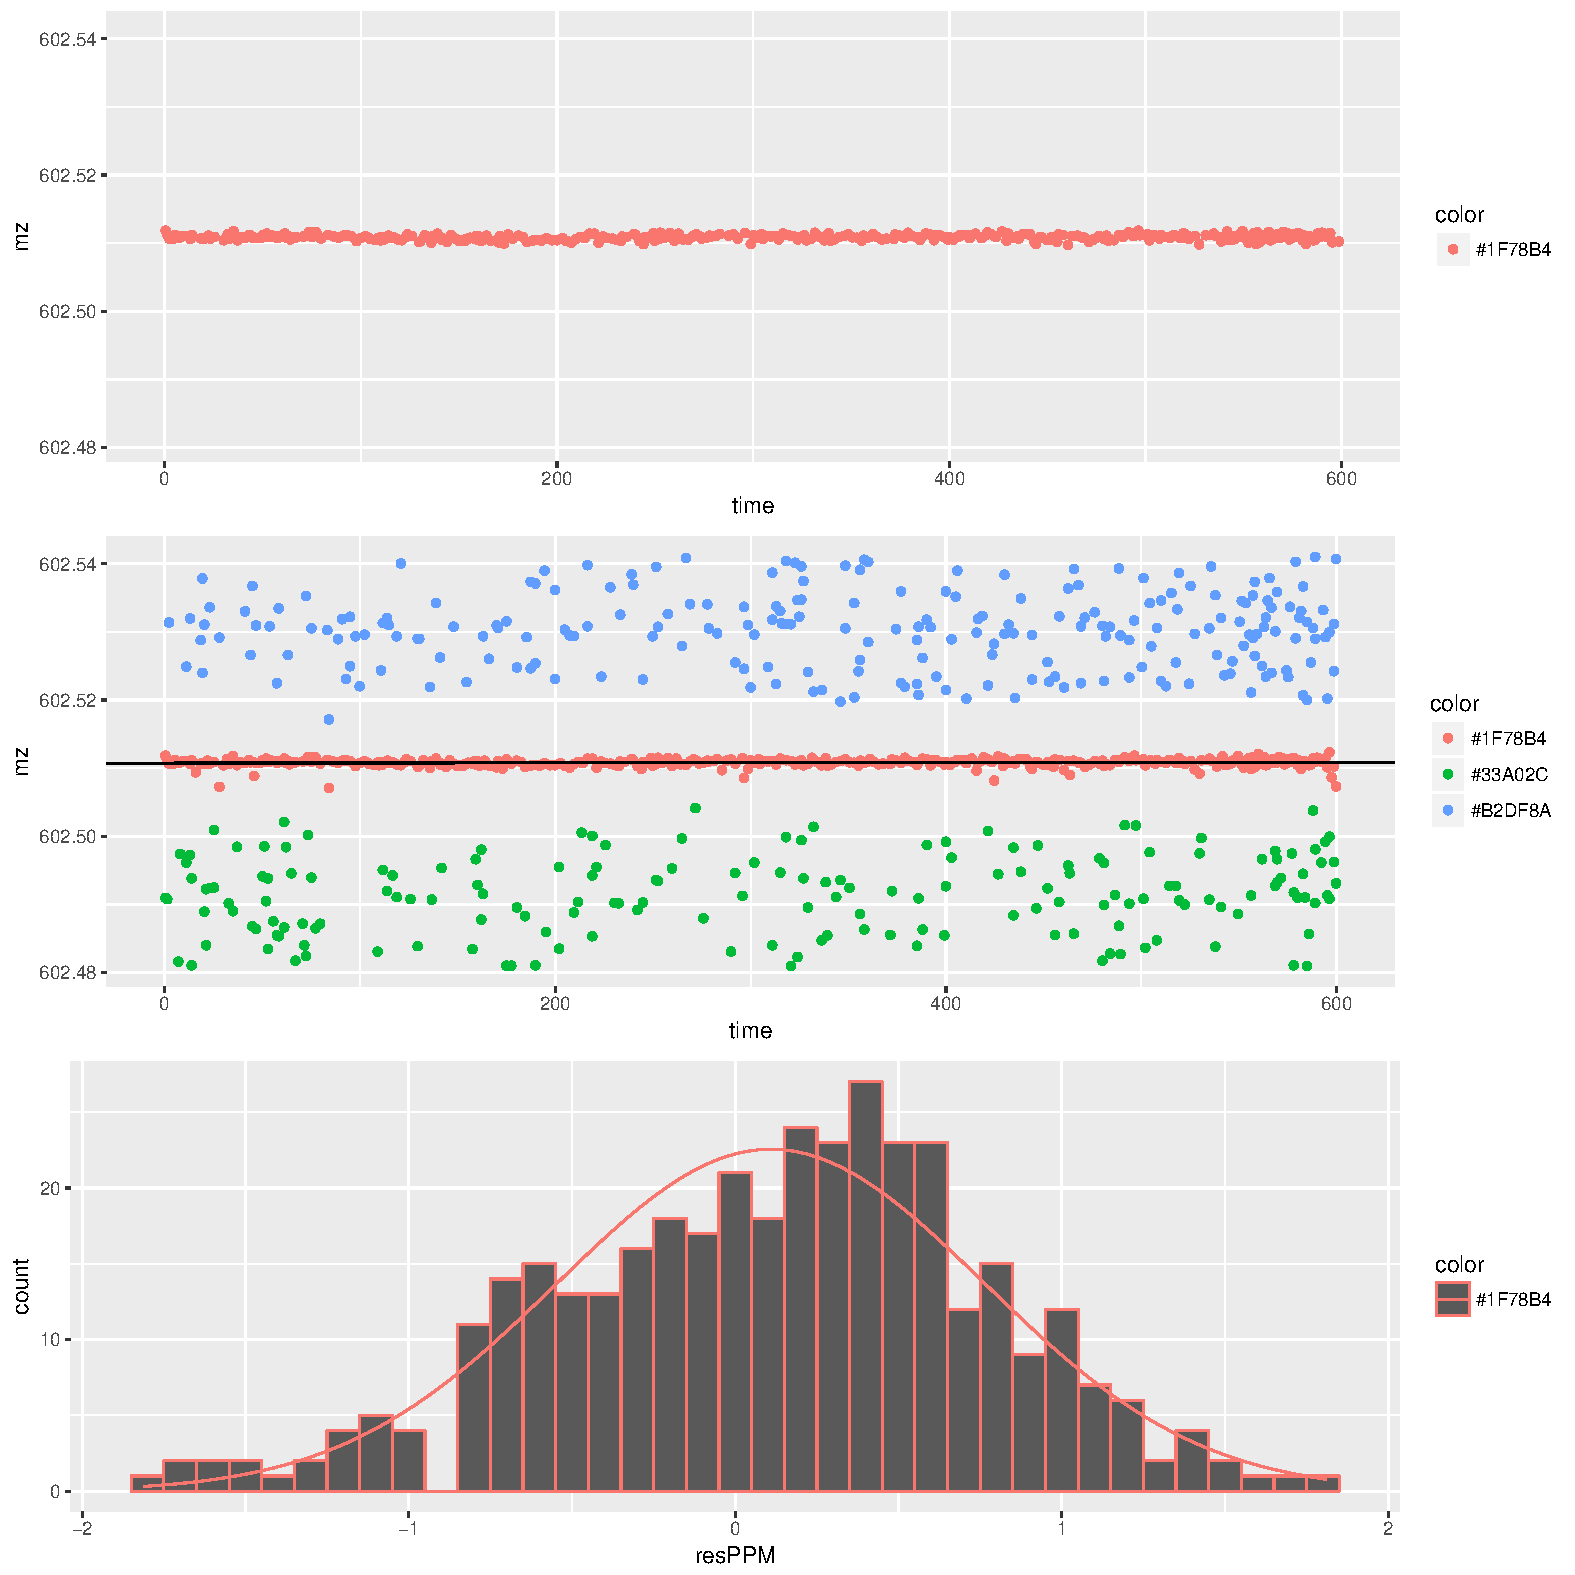
\includegraphics{Supplementary_document_files/figure-latex/filter.lm.602-1.pdf}
NULL

\section{MZ=174.051}\label{mz174.051}

\begin{Shaded}
\begin{Highlighting}[]
\NormalTok{  idx<-}\KeywordTok{which}\NormalTok{(}\KeywordTok{abs}\NormalTok{(p}\OperatorTok{$}\NormalTok{mz}\OperatorTok{-}\FloatTok{174.051}\NormalTok{)}\OperatorTok{<}\FloatTok{5e-3}\NormalTok{)}
\NormalTok{  cP<-}\KeywordTok{which.max}\NormalTok{(p}\OperatorTok{$}\NormalTok{intensity[idx])}
\NormalTok{  ionI<-idx[cP]}
\NormalTok{  maxMZ<-p}\OperatorTok{$}\NormalTok{mz[ionI]}
\end{Highlighting}
\end{Shaded}

The selected row represents the peak with m/z=174.0472 of the scan N=246
taken at time 407.9 sec:

\begin{Shaded}
\begin{Highlighting}[]
\KeywordTok{print}\NormalTok{(}\KeywordTok{getScanPlot}\NormalTok{(p[scan}\OperatorTok{==}\NormalTok{p}\OperatorTok{$}\NormalTok{scan[ionI]]))}
\end{Highlighting}
\end{Shaded}

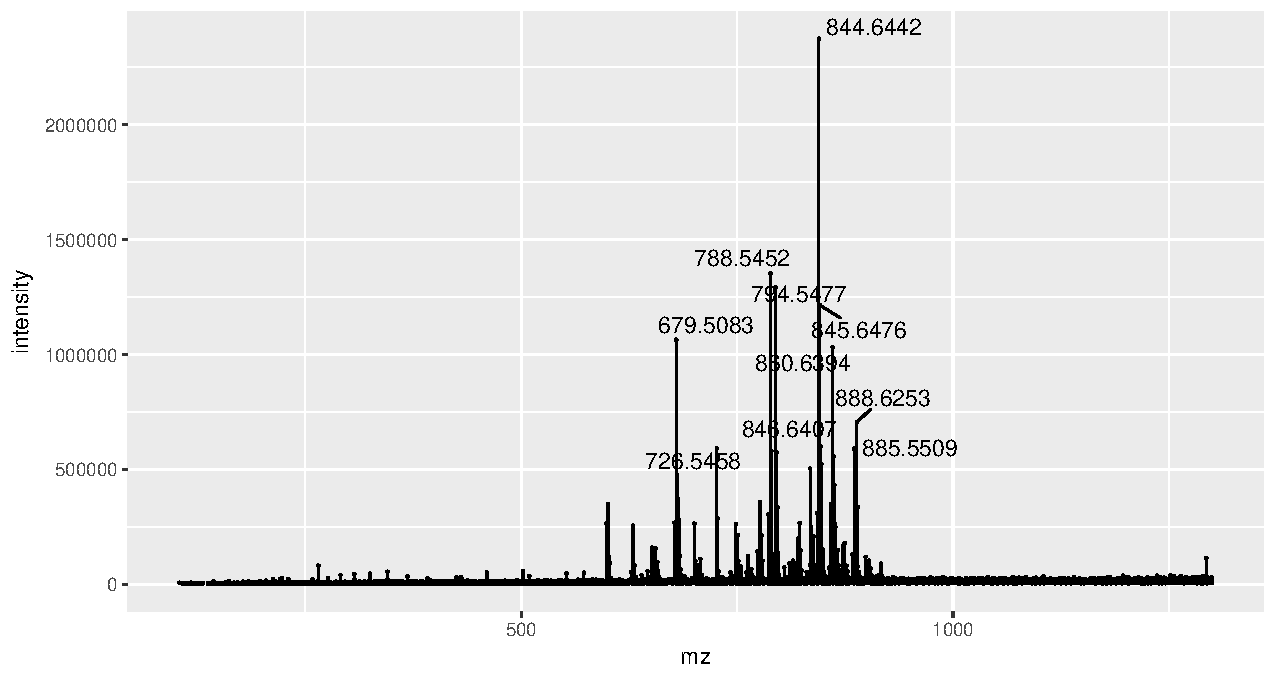
\includegraphics{Supplementary_document_files/figure-latex/ion.plots.174-1.pdf}

Now we collect all signals in the vicinity (50 ppm) of the selected m/z
value and analyze how they drift with time:

\begin{Shaded}
\begin{Highlighting}[]
\NormalTok{  idx <-}\StringTok{ }\KeywordTok{which}\NormalTok{(}\KeywordTok{abs}\NormalTok{(p}\OperatorTok{$}\NormalTok{mz }\OperatorTok{-}\StringTok{ }\NormalTok{maxMZ) }\OperatorTok{<}\StringTok{ }\NormalTok{(ppm }\OperatorTok{*}\StringTok{ }\FloatTok{1e-6} \OperatorTok{*}\StringTok{ }\NormalTok{maxMZ))}
\NormalTok{  p. <-}\StringTok{ }\NormalTok{p[idx, ]}
\end{Highlighting}
\end{Shaded}

To separate feature from surrounding noise we cluster data in m/z domain
by hierarchical Ward clustering and select the most stable clusters with
dynamicTreeCut:

\begin{Shaded}
\begin{Highlighting}[]
\NormalTok{  dissim1 =}\StringTok{ }\KeywordTok{dist}\NormalTok{(p.}\OperatorTok{$}\NormalTok{mz)}
\NormalTok{  dendro1 <-}\StringTok{ }\KeywordTok{hclust}\NormalTok{(}\DataTypeTok{d =}\NormalTok{ dissim1, }\DataTypeTok{method =} \StringTok{'ward.D2'}\NormalTok{)}
\NormalTok{  ct1 <-}\StringTok{ }\KeywordTok{cutreeDynamic}\NormalTok{(}
\NormalTok{    dendro1,}
    \DataTypeTok{cutHeight =} \OtherTok{NULL}\NormalTok{,}
    \DataTypeTok{minClusterSize =} \DecValTok{30}\NormalTok{,}
    \DataTypeTok{method =} \StringTok{"hybrid"}\NormalTok{,}
    \DataTypeTok{deepSplit =} \DecValTok{0}\NormalTok{,}
    \DataTypeTok{pamStage =} \OtherTok{TRUE}\NormalTok{,}
    \DataTypeTok{distM =} \KeywordTok{as.matrix}\NormalTok{(dissim1),}
    \DataTypeTok{maxPamDist =} \DecValTok{0}\NormalTok{,}
    \DataTypeTok{verbose =} \DecValTok{0}
\NormalTok{  )}
\NormalTok{  cct1 <-}\StringTok{ }\NormalTok{ct1[}\KeywordTok{which.max}\NormalTok{(p.}\OperatorTok{$}\NormalTok{intensity)]}
\NormalTok{  id.}\DecValTok{1}\NormalTok{ <-}\StringTok{ }\NormalTok{idx[ct1 }\OperatorTok{==}\StringTok{ }\NormalTok{cct1]}
\NormalTok{  mz1 <-}\StringTok{ }\KeywordTok{median}\NormalTok{(p}\OperatorTok{$}\NormalTok{mz[id.}\DecValTok{1}\NormalTok{])}
\NormalTok{  p.}\OperatorTok{$}\NormalTok{color<-.pal[ct1}\OperatorTok{+}\DecValTok{1}\NormalTok{]}
\NormalTok{  rl <-}\StringTok{ }\KeywordTok{get_runLen}\NormalTok{(p}\OperatorTok{$}\NormalTok{scan[id.}\DecValTok{1}\NormalTok{], scanLen)}
\NormalTok{  p1<-}\KeywordTok{qplot}\NormalTok{(time,intensity,}\DataTypeTok{data =}\NormalTok{ p.,}\DataTypeTok{main=}\KeywordTok{paste0}\NormalTok{(}\StringTok{'mz'}\NormalTok{,maxMZ),}\DataTypeTok{log=}\StringTok{'y'}\NormalTok{,}\DataTypeTok{color=}\NormalTok{color)}
\NormalTok{  p2<-}\KeywordTok{qplot}\NormalTok{(time,mz,}\DataTypeTok{data =}\NormalTok{ p.,}\DataTypeTok{color=}\NormalTok{color)}
\NormalTok{  p3<-}\KeywordTok{qplot}\NormalTok{(mz,intensity,}\DataTypeTok{data =}\NormalTok{ p.,}\DataTypeTok{color=}\NormalTok{color)}
  \KeywordTok{print}\NormalTok{(}\KeywordTok{multiplot}\NormalTok{(p1, p2, p3, }\DataTypeTok{cols=}\DecValTok{1}\NormalTok{))}
\end{Highlighting}
\end{Shaded}

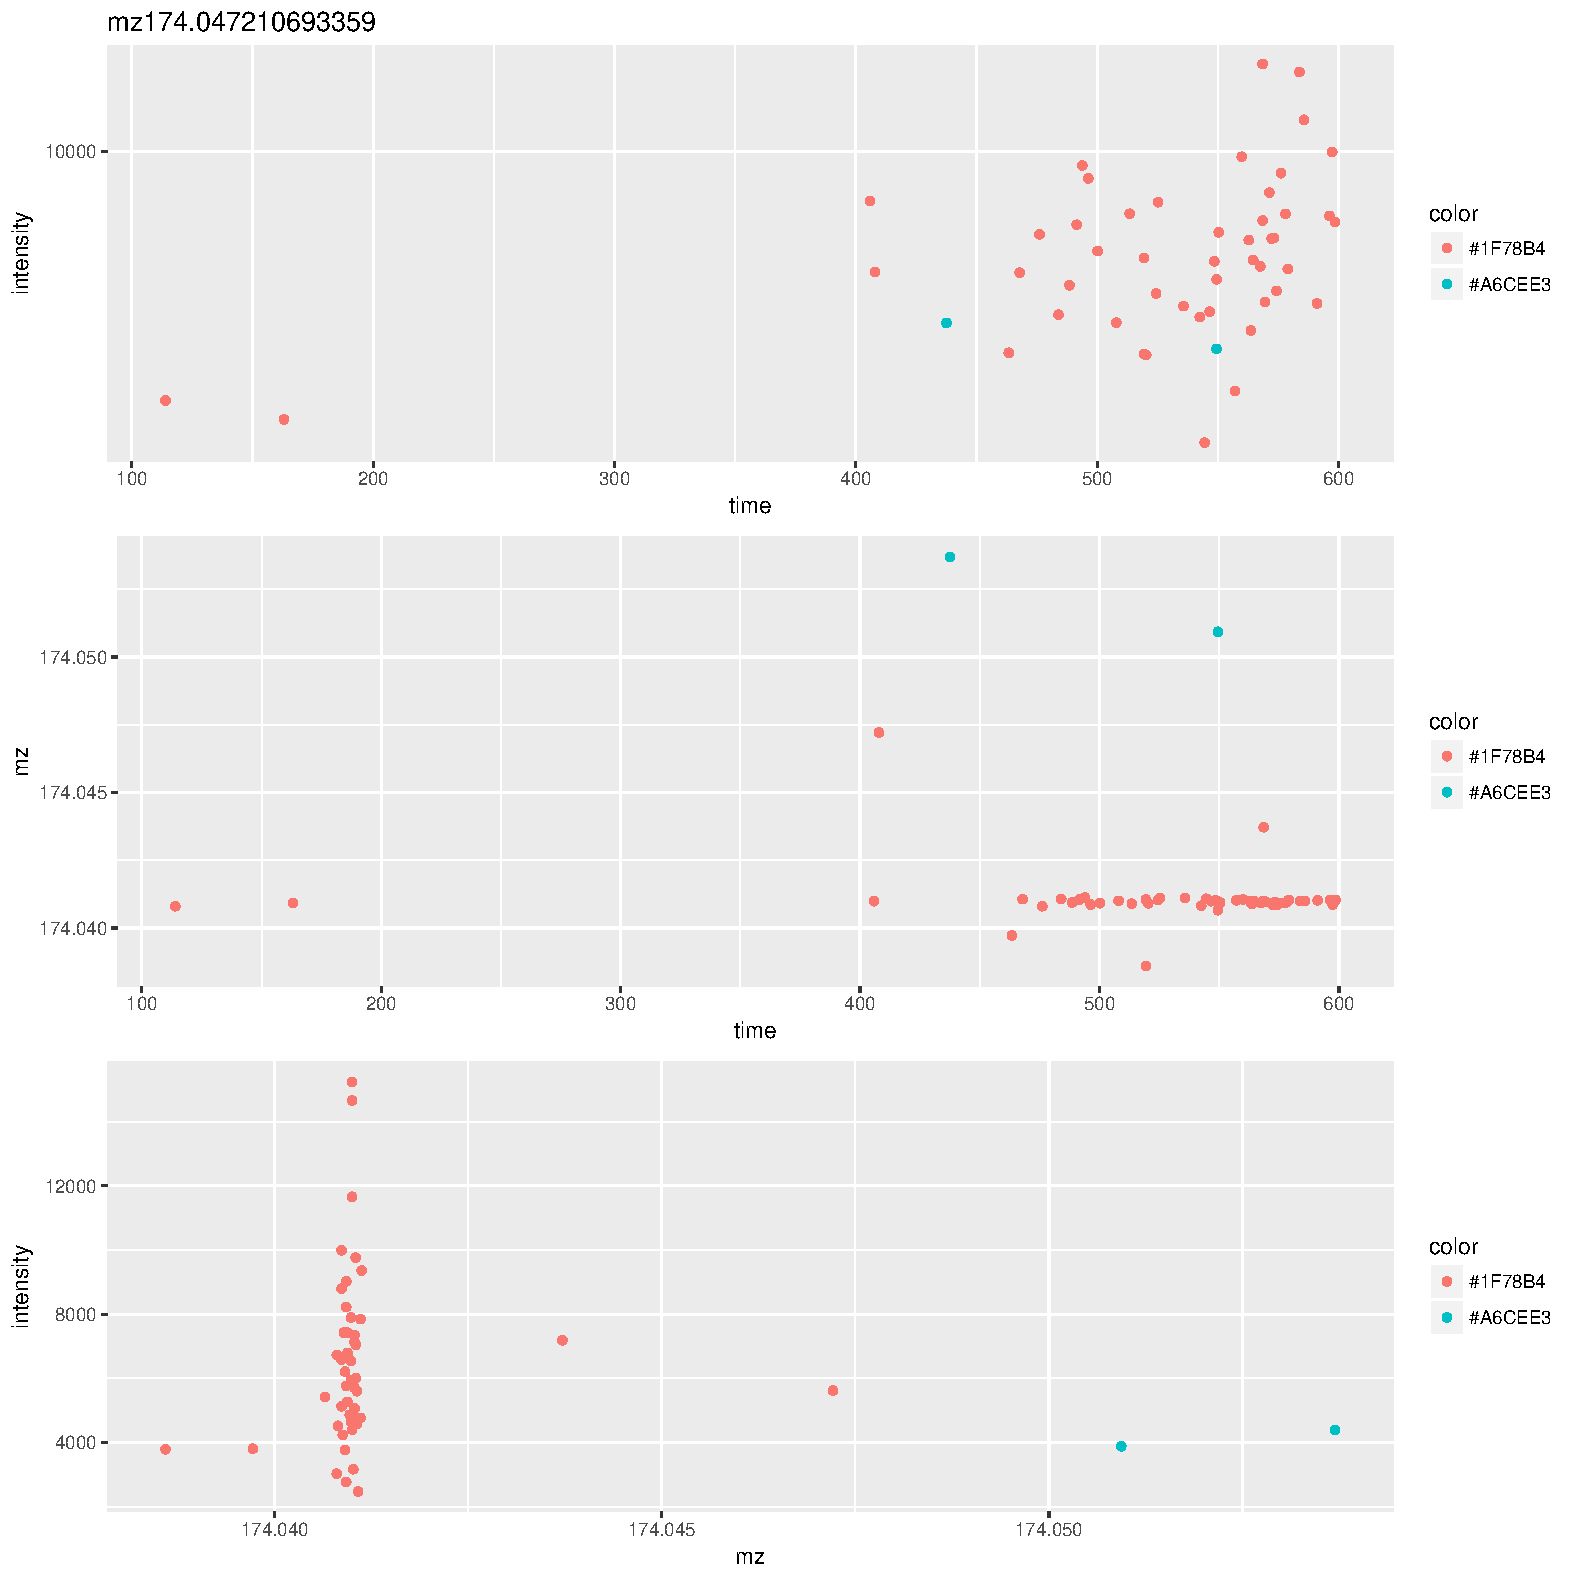
\includegraphics{Supplementary_document_files/figure-latex/cluster.mz.174-1.pdf}
NULL

\begin{Shaded}
\begin{Highlighting}[]
\NormalTok{  l<-}\KeywordTok{lm}\NormalTok{(mz }\OperatorTok{~}\StringTok{ }\NormalTok{time, }\DataTypeTok{data =}\NormalTok{ p[id.}\DecValTok{1}\NormalTok{, ])}
\ControlFlowTok{if}\NormalTok{ (}\KeywordTok{all}\NormalTok{(}\OperatorTok{!}\KeywordTok{is.na}\NormalTok{(l}\OperatorTok{$}\NormalTok{coefficients))) \{}
\NormalTok{  op <-}\StringTok{ }\KeywordTok{par}\NormalTok{(}\DataTypeTok{mfrow =} \KeywordTok{c}\NormalTok{(}\DecValTok{2}\NormalTok{, }\DecValTok{2}\NormalTok{), }\DataTypeTok{oma =} \KeywordTok{c}\NormalTok{(}\DecValTok{0}\NormalTok{, }\DecValTok{0}\NormalTok{, }\DecValTok{2}\NormalTok{, }\DecValTok{0}\NormalTok{))}
  \KeywordTok{plot}\NormalTok{(l)}
  \KeywordTok{par}\NormalTok{(op)}
\NormalTok{\}}
\end{Highlighting}
\end{Shaded}

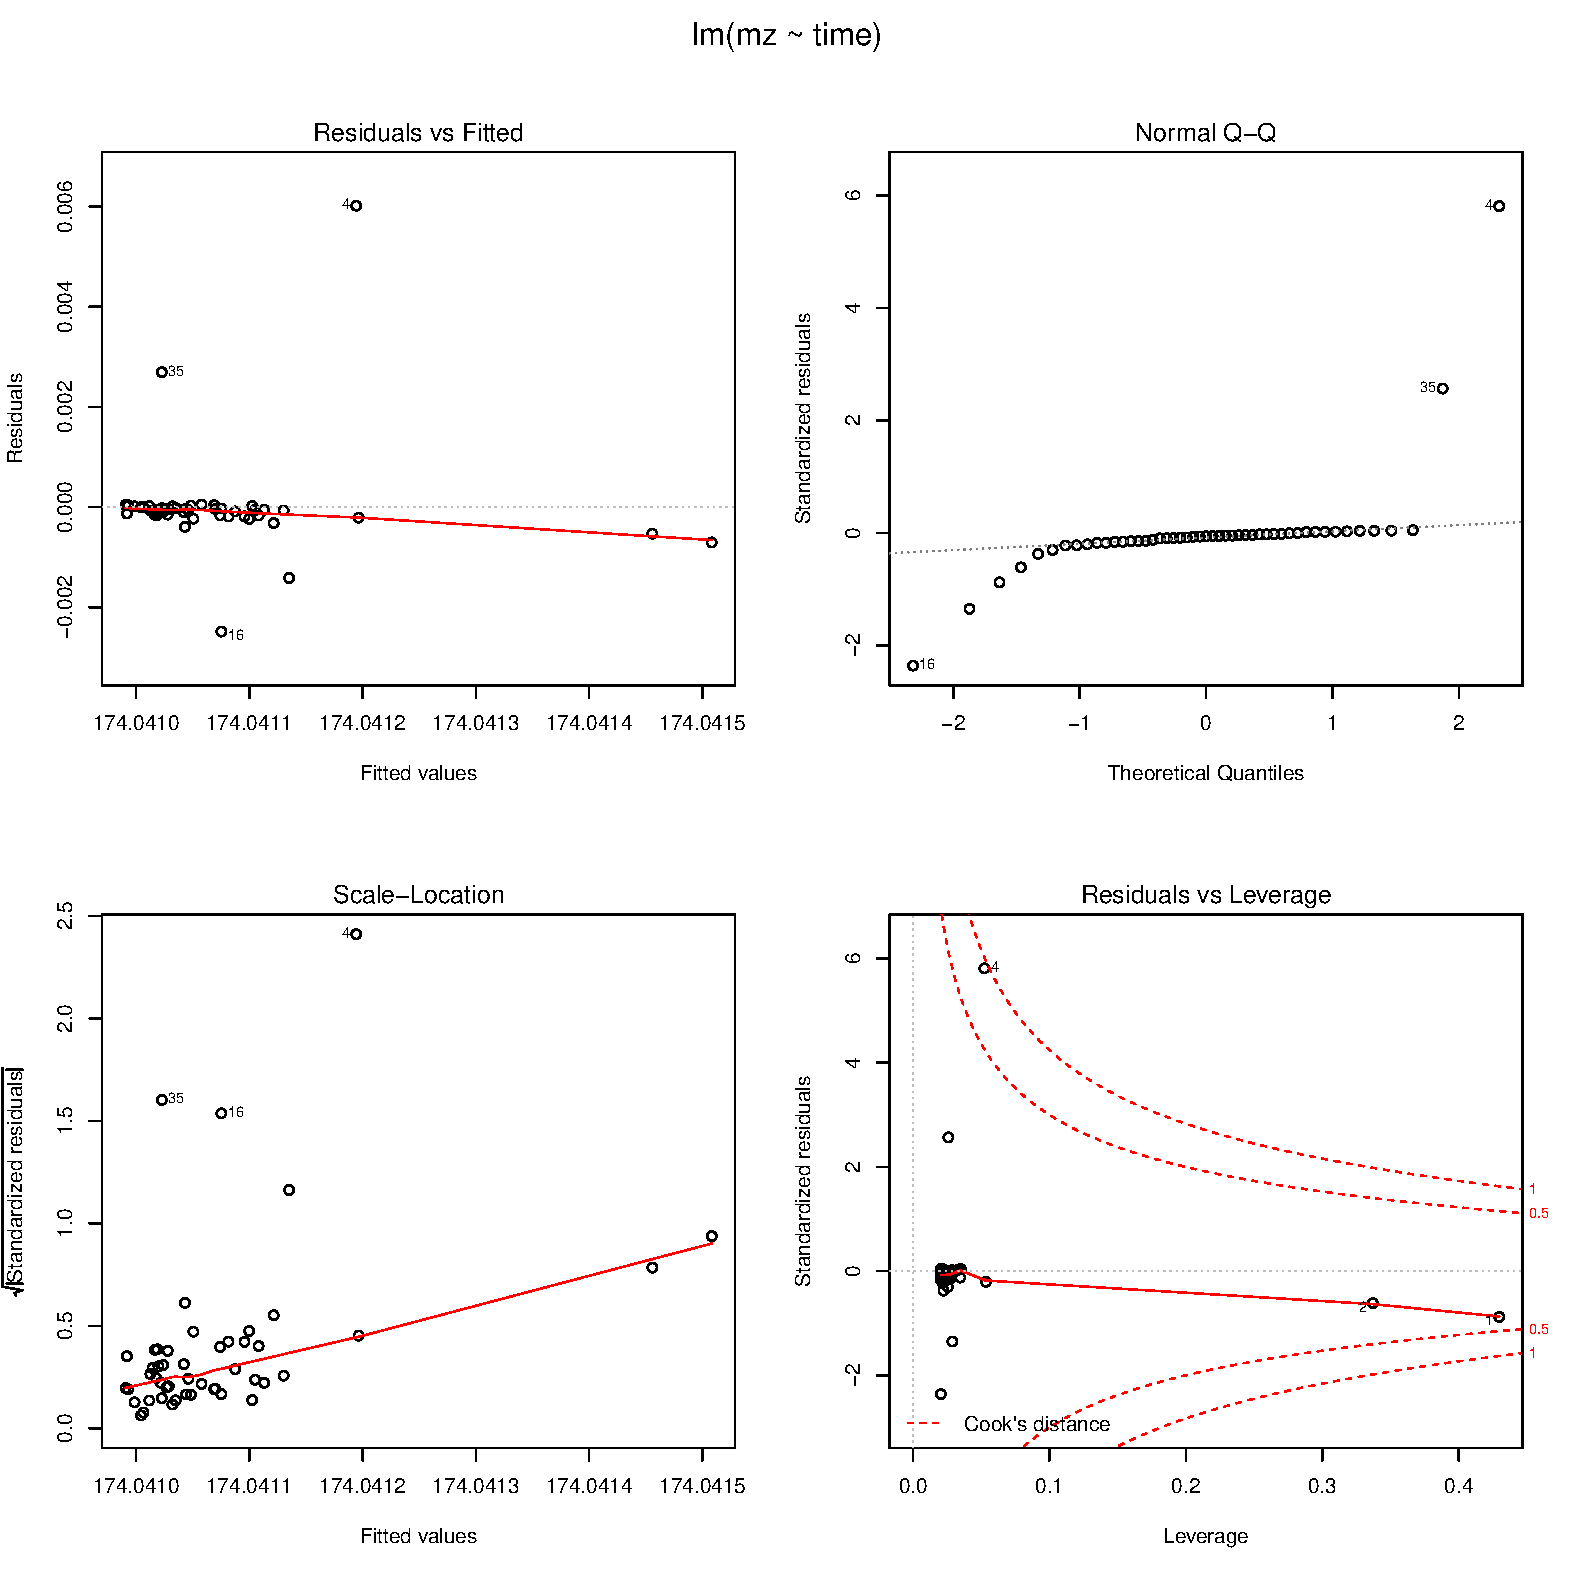
\includegraphics{Supplementary_document_files/figure-latex/fit.lin.174-1.pdf}

\begin{Shaded}
\begin{Highlighting}[]
\ControlFlowTok{if}\NormalTok{ (}\KeywordTok{all}\NormalTok{(}\OperatorTok{!}\KeywordTok{is.na}\NormalTok{(l}\OperatorTok{$}\NormalTok{coefficients))) \{}
  \KeywordTok{range}\NormalTok{(l}\OperatorTok{$}\NormalTok{residuals[}\KeywordTok{abs}\NormalTok{(}\KeywordTok{rstandard}\NormalTok{(l)) }\OperatorTok{<=}\StringTok{ }\DecValTok{2}\NormalTok{]) ->}\StringTok{ }\NormalTok{bnd}
\NormalTok{  pl <-}\StringTok{ }\KeywordTok{predict}\NormalTok{(l, p.)}
\NormalTok{  rl <-}\StringTok{ }\NormalTok{p.}\OperatorTok{$}\NormalTok{mz }\OperatorTok{-}\StringTok{ }\NormalTok{pl}
\NormalTok{  idL <-}\StringTok{ }\KeywordTok{which}\NormalTok{(rl }\OperatorTok{>=}\StringTok{ }\NormalTok{bnd[}\DecValTok{1}\NormalTok{] }\OperatorTok{&}\StringTok{ }\NormalTok{rl }\OperatorTok{<=}\StringTok{ }\NormalTok{bnd[}\DecValTok{2}\NormalTok{])}
\NormalTok{  p5 =}\StringTok{ }\KeywordTok{qplot}\NormalTok{(}
\NormalTok{          time,}
\NormalTok{          mz,}
          \DataTypeTok{data =}\NormalTok{ p.[idL],}
          \DataTypeTok{color =}\NormalTok{ color,}
          \DataTypeTok{xlim =} \KeywordTok{range}\NormalTok{(p.}\OperatorTok{$}\NormalTok{time),}
          \DataTypeTok{ylim =} \KeywordTok{range}\NormalTok{(p.}\OperatorTok{$}\NormalTok{mz)}
\NormalTok{  )}
\NormalTok{  p6 =}\StringTok{ }\KeywordTok{qplot}\NormalTok{(time,}
\NormalTok{          mz,}
          \DataTypeTok{data =}\NormalTok{ p.,}
          \DataTypeTok{color =}\NormalTok{ color) }\OperatorTok{+}
\StringTok{      }\KeywordTok{geom_abline}\NormalTok{(}\DataTypeTok{intercept =}\NormalTok{ l}\OperatorTok{$}\NormalTok{coefficients[}\DecValTok{1}\NormalTok{],}
          \DataTypeTok{slope =}\NormalTok{ l}\OperatorTok{$}\NormalTok{coefficients[}\DecValTok{2}\NormalTok{])}
  
  
\NormalTok{  p.}\OperatorTok{$}\NormalTok{resPPM<-rl}\OperatorTok{*}\FloatTok{1e6}\OperatorTok{/}\NormalTok{l}\OperatorTok{$}\NormalTok{coefficients[}\DecValTok{1}\NormalTok{]}
\NormalTok{  p7<-}\KeywordTok{qplot}\NormalTok{(resPPM,}\DataTypeTok{data=}\NormalTok{p.[idL],}
            \DataTypeTok{binwidth=}\NormalTok{binwidth,}\DataTypeTok{color=}\NormalTok{color)}\OperatorTok{+}
\StringTok{    }\KeywordTok{stat_function}\NormalTok{(}\DataTypeTok{fun =} \ControlFlowTok{function}\NormalTok{(x, mean, sd, n, bw)\{}
      \KeywordTok{dnorm}\NormalTok{(}\DataTypeTok{x =}\NormalTok{ x, }\DataTypeTok{mean =}\NormalTok{ mean, }\DataTypeTok{sd =}\NormalTok{ sd) }\OperatorTok{*}\StringTok{ }\NormalTok{n }\OperatorTok{*}\StringTok{ }\NormalTok{bw}
\NormalTok{      \},}
      \DataTypeTok{args =} \KeywordTok{c}\NormalTok{(}\DataTypeTok{mean =} \KeywordTok{mean}\NormalTok{(p.}\OperatorTok{$}\NormalTok{resPPM[idL]), }
               \DataTypeTok{sd =} \KeywordTok{sd}\NormalTok{(p.}\OperatorTok{$}\NormalTok{resPPM[idL]), }
               \DataTypeTok{n =} \KeywordTok{length}\NormalTok{(idL), }
               \DataTypeTok{bw =}\NormalTok{ binwidth))}

  \KeywordTok{print}\NormalTok{(}\KeywordTok{multiplot}\NormalTok{(p5, p6, p7, }\DataTypeTok{cols =} \DecValTok{1}\NormalTok{))}
\NormalTok{\}}
\end{Highlighting}
\end{Shaded}

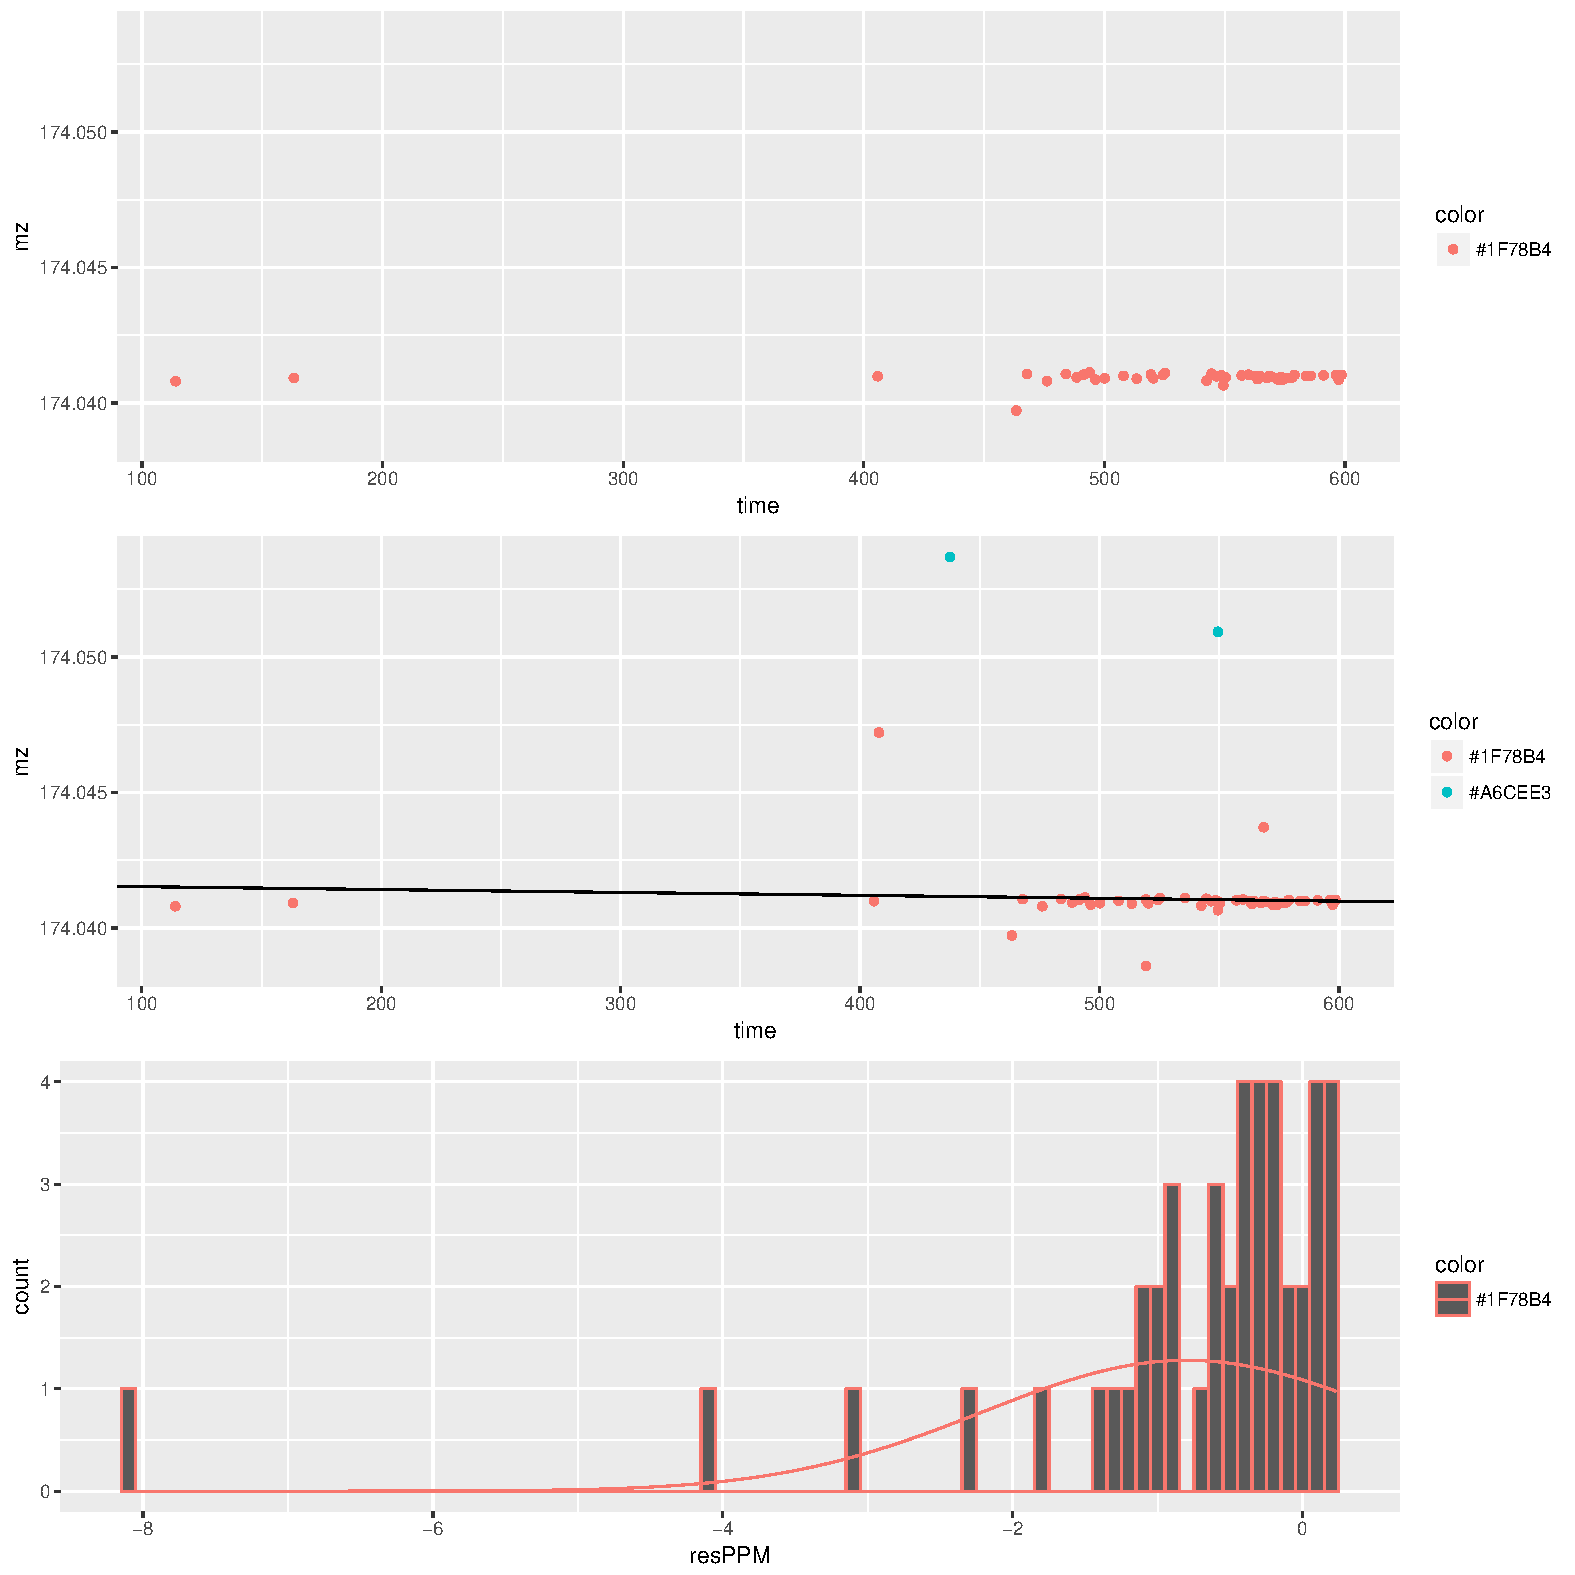
\includegraphics{Supplementary_document_files/figure-latex/filter.lm.174-1.pdf}
NULL

\section{Appendix}\label{appendix}

\subsection{Custom Functions}\label{custom-functions}

\begin{Shaded}
\begin{Highlighting}[]
\NormalTok{## Custom functions used in the analysis should go into this chunk.}
\NormalTok{## They will be listed in their own section of the appendix.}
\NormalTok{makePeaks<-}\ControlFlowTok{function}\NormalTok{(.xcms)\{}
  \CommentTok{# this function converts XCMSRaw data into mz table}
\NormalTok{    sel <-}\StringTok{ }\KeywordTok{profRange}\NormalTok{(.xcms)}
\NormalTok{    peaks<-}\KeywordTok{data.frame}\NormalTok{(}\DataTypeTok{mz=}\FloatTok{100.0}\NormalTok{,}
                      \DataTypeTok{intensity=}\FloatTok{1.0e6}\NormalTok{,}
                      \DataTypeTok{ion=}\OtherTok{NA}\NormalTok{,}
                      \DataTypeTok{MP=}\OtherTok{NA}\NormalTok{,}
                      \DataTypeTok{time=}\FloatTok{0.0}\NormalTok{,}
                      \DataTypeTok{scan=}\DecValTok{1}\NormalTok{,}
                      \DataTypeTok{delta=}\OtherTok{NA}\NormalTok{,}
                      \DataTypeTok{adduct=}\OtherTok{NA}\NormalTok{)[}\OtherTok{FALSE}\NormalTok{,]}
\NormalTok{    l<-}\KeywordTok{list}\NormalTok{()}
\NormalTok{    l<-}\KeywordTok{lapply}\NormalTok{(sel}\OperatorTok{$}\NormalTok{scanidx,}\ControlFlowTok{function}\NormalTok{(i)\{}
\NormalTok{        scan <-}\StringTok{ }\KeywordTok{as.data.table}\NormalTok{(}\KeywordTok{getScan}\NormalTok{(xraw, sel}\OperatorTok{$}\NormalTok{scanidx[i], sel}\OperatorTok{$}\NormalTok{mzrange))}
\NormalTok{        p<-scan}
\NormalTok{        p}\OperatorTok{$}\NormalTok{ion<-}\OtherTok{NA}
\NormalTok{        p}\OperatorTok{$}\NormalTok{time<-xraw}\OperatorTok{@}\NormalTok{scantime[i]}
\NormalTok{        p}\OperatorTok{$}\NormalTok{scan<-i}
        \KeywordTok{return}\NormalTok{(p)}
\NormalTok{    \})}
\NormalTok{    peaks<-}\KeywordTok{as.data.table}\NormalTok{(}\KeywordTok{ldply}\NormalTok{(l,rbind))}
    \KeywordTok{return}\NormalTok{(peaks)}
\NormalTok{\}}
\NormalTok{getScanPlot<-}\ControlFlowTok{function}\NormalTok{(mz1)\{}
\NormalTok{  mzp<-mz1}
\NormalTok{  mzp[,lab}\OperatorTok{:}\ErrorTok{=}\KeywordTok{paste}\NormalTok{(}\KeywordTok{round}\NormalTok{(mz,}\DecValTok{4}\NormalTok{))]}
\NormalTok{  mzp[}\KeywordTok{order}\NormalTok{(intensity,}\DataTypeTok{decreasing =} \OtherTok{TRUE}\NormalTok{)[}\OperatorTok{-}\KeywordTok{c}\NormalTok{(}\DecValTok{1}\OperatorTok{:}\DecValTok{10}\NormalTok{)],lab}\OperatorTok{:}\ErrorTok{=}\StringTok{''}\NormalTok{]}
\NormalTok{  p<-}\KeywordTok{ggplot}\NormalTok{(mzp, }\KeywordTok{aes}\NormalTok{(}\DataTypeTok{x=}\NormalTok{mz,}\DataTypeTok{yend=}\DecValTok{0}\NormalTok{,}\DataTypeTok{xend=}\NormalTok{mz, }\DataTypeTok{y=}\NormalTok{intensity)) }\OperatorTok{+}
\StringTok{    }\KeywordTok{geom_segment}\NormalTok{()}\OperatorTok{+}\KeywordTok{geom_point}\NormalTok{(}\DataTypeTok{size=}\FloatTok{0.15}\NormalTok{) }\OperatorTok{+}\StringTok{ }\CommentTok{#scale_y_log10()+}
\StringTok{    }\KeywordTok{geom_text_repel}\NormalTok{(}\KeywordTok{aes}\NormalTok{(}\DataTypeTok{x =}\NormalTok{ mz,}\DataTypeTok{y=}\NormalTok{intensity,}\DataTypeTok{label=}\NormalTok{lab))}\OperatorTok{+}
\StringTok{    }\KeywordTok{theme}\NormalTok{(}\DataTypeTok{legend.position=}\StringTok{"none"}\NormalTok{)}
  \KeywordTok{return}\NormalTok{(p)}
\NormalTok{\}}

\CommentTok{# Multiple plot function}
\CommentTok{#}
\CommentTok{# ggplot objects can be passed in ..., or to plotlist (as a list of ggplot objects)}
\CommentTok{# - cols:   Number of columns in layout}
\CommentTok{# - layout: A matrix specifying the layout. If present, 'cols' is ignored.}
\CommentTok{#}
\CommentTok{# If the layout is something like matrix(c(1,2,3,3), nrow=2, byrow=TRUE),}
\CommentTok{# then plot 1 will go in the upper left, 2 will go in the upper right, and}
\CommentTok{# 3 will go all the way across the bottom.}
\CommentTok{# }
\CommentTok{# Code is taken from http://www.cookbook-r.com/Graphs/Multiple_graphs_on_one_page_%28ggplot2%29/}
\CommentTok{#}
\NormalTok{multiplot <-}\StringTok{ }\ControlFlowTok{function}\NormalTok{(..., }\DataTypeTok{plotlist=}\OtherTok{NULL}\NormalTok{, file, }\DataTypeTok{cols=}\DecValTok{1}\NormalTok{, }\DataTypeTok{layout=}\OtherTok{NULL}\NormalTok{) \{}
  \KeywordTok{library}\NormalTok{(grid)}

  \CommentTok{# Make a list from the ... arguments and plotlist}
\NormalTok{  plots <-}\StringTok{ }\KeywordTok{c}\NormalTok{(}\KeywordTok{list}\NormalTok{(...), plotlist)}

\NormalTok{  numPlots =}\StringTok{ }\KeywordTok{length}\NormalTok{(plots)}

  \CommentTok{# If layout is NULL, then use 'cols' to determine layout}
  \ControlFlowTok{if}\NormalTok{ (}\KeywordTok{is.null}\NormalTok{(layout)) \{}
    \CommentTok{# Make the panel}
    \CommentTok{# ncol: Number of columns of plots}
    \CommentTok{# nrow: Number of rows needed, calculated from # of cols}
\NormalTok{    layout <-}\StringTok{ }\KeywordTok{matrix}\NormalTok{(}\KeywordTok{seq}\NormalTok{(}\DecValTok{1}\NormalTok{, cols }\OperatorTok{*}\StringTok{ }\KeywordTok{ceiling}\NormalTok{(numPlots}\OperatorTok{/}\NormalTok{cols)),}
                    \DataTypeTok{ncol =}\NormalTok{ cols, }\DataTypeTok{nrow =} \KeywordTok{ceiling}\NormalTok{(numPlots}\OperatorTok{/}\NormalTok{cols))}
\NormalTok{  \}}

 \ControlFlowTok{if}\NormalTok{ (numPlots}\OperatorTok{==}\DecValTok{1}\NormalTok{) \{}
    \KeywordTok{print}\NormalTok{(plots[[}\DecValTok{1}\NormalTok{]])}

\NormalTok{  \} }\ControlFlowTok{else}\NormalTok{ \{}
    \CommentTok{# Set up the page}
    \KeywordTok{grid.newpage}\NormalTok{()}
    \KeywordTok{pushViewport}\NormalTok{(}\KeywordTok{viewport}\NormalTok{(}\DataTypeTok{layout =} \KeywordTok{grid.layout}\NormalTok{(}\KeywordTok{nrow}\NormalTok{(layout), }\KeywordTok{ncol}\NormalTok{(layout))))}

    \CommentTok{# Make each plot, in the correct location}
    \ControlFlowTok{for}\NormalTok{ (i }\ControlFlowTok{in} \DecValTok{1}\OperatorTok{:}\NormalTok{numPlots) \{}
      \CommentTok{# Get the i,j matrix positions of the regions that contain this subplot}
\NormalTok{      matchidx <-}\StringTok{ }\KeywordTok{as.data.frame}\NormalTok{(}\KeywordTok{which}\NormalTok{(layout }\OperatorTok{==}\StringTok{ }\NormalTok{i, }\DataTypeTok{arr.ind =} \OtherTok{TRUE}\NormalTok{))}

      \KeywordTok{print}\NormalTok{(plots[[i]], }\DataTypeTok{vp =} \KeywordTok{viewport}\NormalTok{(}\DataTypeTok{layout.pos.row =}\NormalTok{ matchidx}\OperatorTok{$}\NormalTok{row,}
                                      \DataTypeTok{layout.pos.col =}\NormalTok{ matchidx}\OperatorTok{$}\NormalTok{col))}
\NormalTok{    \}}
\NormalTok{  \}}
\NormalTok{\}}

\NormalTok{get_Rle<-}\ControlFlowTok{function}\NormalTok{(.scan,.max)\{}
    \KeywordTok{require}\NormalTok{(IRanges)}
\NormalTok{  xf <-}\StringTok{ }\KeywordTok{rep}\NormalTok{(}\DecValTok{0}\NormalTok{, .max)}
\NormalTok{  xf[.scan] <-}\StringTok{ }\DecValTok{1}
  \KeywordTok{Rle}\NormalTok{(xf) ->}\StringTok{ }\NormalTok{r}
  \KeywordTok{return}\NormalTok{(r)}
\NormalTok{\}}

\NormalTok{get_runLen <-}\StringTok{ }\ControlFlowTok{function}\NormalTok{(.scan, .max) \{}
\NormalTok{  r<-}\KeywordTok{get_Rle}\NormalTok{(.scan,.max)}
  \KeywordTok{return}\NormalTok{(}\KeywordTok{runLength}\NormalTok{(r)[}\KeywordTok{which}\NormalTok{(}\KeywordTok{runValue}\NormalTok{(r)}\OperatorTok{==}\DecValTok{1}\NormalTok{)])}
\NormalTok{\}}

\NormalTok{getFeature<-}\ControlFlowTok{function}\NormalTok{(l,p.,}\DataTypeTok{th=}\FloatTok{2.0}\NormalTok{)\{}
  \KeywordTok{range}\NormalTok{(l}\OperatorTok{$}\NormalTok{residuals[}\KeywordTok{abs}\NormalTok{(}\KeywordTok{rstandard}\NormalTok{(l)) }\OperatorTok{<=}\StringTok{ }\DecValTok{2}\NormalTok{]) ->}\StringTok{ }\NormalTok{bnd}
\NormalTok{  pl <-}\StringTok{ }\KeywordTok{predict}\NormalTok{(l, p.)}
\NormalTok{  rl <-}\StringTok{ }\NormalTok{p.}\OperatorTok{$}\NormalTok{mz }\OperatorTok{-}\StringTok{ }\NormalTok{pl}
\NormalTok{  idL <-}\StringTok{ }\KeywordTok{which}\NormalTok{(rl }\OperatorTok{>=}\StringTok{ }\NormalTok{bnd[}\DecValTok{1}\NormalTok{] }\OperatorTok{&}\StringTok{ }\NormalTok{rl }\OperatorTok{<=}\StringTok{ }\NormalTok{bnd[}\DecValTok{2}\NormalTok{])}
  \KeywordTok{return}\NormalTok{(idL)}
\NormalTok{\}}
\end{Highlighting}
\end{Shaded}

\subsection{Version}\label{version}

\subsubsection{Document version}\label{document-version}

e807239b6e-dirty 20.06.2017

\subsubsection{Session Info}\label{session-info}

\begin{itemize}
\item
  \textbf{platform}:

  \begin{itemize}
  \tightlist
  \item
    \textbf{version}: R version 3.3.2 (2016-10-31)
  \item
    \textbf{system}: x86\_64, darwin13.4.0
  \item
    \textbf{ui}: X11
  \item
    \textbf{language}: (EN)
  \item
    \textbf{collate}: en\_US.UTF-8
  \item
    \textbf{tz}: Europe/Minsk
  \item
    \textbf{date}: 2017-06-15
  \end{itemize}
\item
  \textbf{packages}:

  \begin{longtable}[]{@{}ccccc@{}}
  \toprule
  \begin{minipage}[b]{0.13\columnwidth}\centering\strut
  package\strut
  \end{minipage} & \begin{minipage}[b]{0.05\columnwidth}\centering\strut
  *\strut
  \end{minipage} & \begin{minipage}[b]{0.13\columnwidth}\centering\strut
  version\strut
  \end{minipage} & \begin{minipage}[b]{0.13\columnwidth}\centering\strut
  date\strut
  \end{minipage} & \begin{minipage}[b]{0.29\columnwidth}\centering\strut
  source\strut
  \end{minipage}\tabularnewline
  \midrule
  \endhead
  \begin{minipage}[t]{0.13\columnwidth}\centering\strut
  backports\strut
  \end{minipage} & \begin{minipage}[t]{0.05\columnwidth}\centering\strut
  \strut
  \end{minipage} & \begin{minipage}[t]{0.13\columnwidth}\centering\strut
  1.0.5\strut
  \end{minipage} & \begin{minipage}[t]{0.13\columnwidth}\centering\strut
  2017-01-18\strut
  \end{minipage} & \begin{minipage}[t]{0.29\columnwidth}\centering\strut
  CRAN (R 3.3.2)\strut
  \end{minipage}\tabularnewline
  \begin{minipage}[t]{0.13\columnwidth}\centering\strut
  base\strut
  \end{minipage} & \begin{minipage}[t]{0.05\columnwidth}\centering\strut
  *\strut
  \end{minipage} & \begin{minipage}[t]{0.13\columnwidth}\centering\strut
  3.3.2\strut
  \end{minipage} & \begin{minipage}[t]{0.13\columnwidth}\centering\strut
  2016-10-31\strut
  \end{minipage} & \begin{minipage}[t]{0.29\columnwidth}\centering\strut
  local\strut
  \end{minipage}\tabularnewline
  \begin{minipage}[t]{0.13\columnwidth}\centering\strut
  biom\strut
  \end{minipage} & \begin{minipage}[t]{0.05\columnwidth}\centering\strut
  *\strut
  \end{minipage} & \begin{minipage}[t]{0.13\columnwidth}\centering\strut
  0.3.12\strut
  \end{minipage} & \begin{minipage}[t]{0.13\columnwidth}\centering\strut
  2014-02-24\strut
  \end{minipage} & \begin{minipage}[t]{0.29\columnwidth}\centering\strut
  CRAN (R 3.3.0)\strut
  \end{minipage}\tabularnewline
  \begin{minipage}[t]{0.13\columnwidth}\centering\strut
  codetools\strut
  \end{minipage} & \begin{minipage}[t]{0.05\columnwidth}\centering\strut
  \strut
  \end{minipage} & \begin{minipage}[t]{0.13\columnwidth}\centering\strut
  0.2-15\strut
  \end{minipage} & \begin{minipage}[t]{0.13\columnwidth}\centering\strut
  2016-10-05\strut
  \end{minipage} & \begin{minipage}[t]{0.29\columnwidth}\centering\strut
  CRAN (R 3.3.2)\strut
  \end{minipage}\tabularnewline
  \begin{minipage}[t]{0.13\columnwidth}\centering\strut
  colorspace\strut
  \end{minipage} & \begin{minipage}[t]{0.05\columnwidth}\centering\strut
  \strut
  \end{minipage} & \begin{minipage}[t]{0.13\columnwidth}\centering\strut
  1.3-2\strut
  \end{minipage} & \begin{minipage}[t]{0.13\columnwidth}\centering\strut
  2016-12-14\strut
  \end{minipage} & \begin{minipage}[t]{0.29\columnwidth}\centering\strut
  CRAN (R 3.3.2)\strut
  \end{minipage}\tabularnewline
  \begin{minipage}[t]{0.13\columnwidth}\centering\strut
  data.table\strut
  \end{minipage} & \begin{minipage}[t]{0.05\columnwidth}\centering\strut
  *\strut
  \end{minipage} & \begin{minipage}[t]{0.13\columnwidth}\centering\strut
  1.10.4\strut
  \end{minipage} & \begin{minipage}[t]{0.13\columnwidth}\centering\strut
  2017-02-01\strut
  \end{minipage} & \begin{minipage}[t]{0.29\columnwidth}\centering\strut
  CRAN (R 3.3.2)\strut
  \end{minipage}\tabularnewline
  \begin{minipage}[t]{0.13\columnwidth}\centering\strut
  datasets\strut
  \end{minipage} & \begin{minipage}[t]{0.05\columnwidth}\centering\strut
  *\strut
  \end{minipage} & \begin{minipage}[t]{0.13\columnwidth}\centering\strut
  3.3.2\strut
  \end{minipage} & \begin{minipage}[t]{0.13\columnwidth}\centering\strut
  2016-10-31\strut
  \end{minipage} & \begin{minipage}[t]{0.29\columnwidth}\centering\strut
  local\strut
  \end{minipage}\tabularnewline
  \begin{minipage}[t]{0.13\columnwidth}\centering\strut
  devtools\strut
  \end{minipage} & \begin{minipage}[t]{0.05\columnwidth}\centering\strut
  \strut
  \end{minipage} & \begin{minipage}[t]{0.13\columnwidth}\centering\strut
  1.13.1\strut
  \end{minipage} & \begin{minipage}[t]{0.13\columnwidth}\centering\strut
  2017-05-13\strut
  \end{minipage} & \begin{minipage}[t]{0.29\columnwidth}\centering\strut
  CRAN (R 3.3.2)\strut
  \end{minipage}\tabularnewline
  \begin{minipage}[t]{0.13\columnwidth}\centering\strut
  digest\strut
  \end{minipage} & \begin{minipage}[t]{0.05\columnwidth}\centering\strut
  \strut
  \end{minipage} & \begin{minipage}[t]{0.13\columnwidth}\centering\strut
  0.6.12\strut
  \end{minipage} & \begin{minipage}[t]{0.13\columnwidth}\centering\strut
  2017-01-27\strut
  \end{minipage} & \begin{minipage}[t]{0.29\columnwidth}\centering\strut
  CRAN (R 3.3.2)\strut
  \end{minipage}\tabularnewline
  \begin{minipage}[t]{0.13\columnwidth}\centering\strut
  evaluate\strut
  \end{minipage} & \begin{minipage}[t]{0.05\columnwidth}\centering\strut
  \strut
  \end{minipage} & \begin{minipage}[t]{0.13\columnwidth}\centering\strut
  0.10\strut
  \end{minipage} & \begin{minipage}[t]{0.13\columnwidth}\centering\strut
  2016-10-11\strut
  \end{minipage} & \begin{minipage}[t]{0.29\columnwidth}\centering\strut
  CRAN (R 3.3.0)\strut
  \end{minipage}\tabularnewline
  \begin{minipage}[t]{0.13\columnwidth}\centering\strut
  ggplot2\strut
  \end{minipage} & \begin{minipage}[t]{0.05\columnwidth}\centering\strut
  *\strut
  \end{minipage} & \begin{minipage}[t]{0.13\columnwidth}\centering\strut
  2.2.1.9000\strut
  \end{minipage} & \begin{minipage}[t]{0.13\columnwidth}\centering\strut
  2017-06-03\strut
  \end{minipage} & \begin{minipage}[t]{0.29\columnwidth}\centering\strut
  Github
  (\href{mailto:hadley/ggplot2@eedaa81}{\nolinkurl{hadley/ggplot2@eedaa81}})\strut
  \end{minipage}\tabularnewline
  \begin{minipage}[t]{0.13\columnwidth}\centering\strut
  graphics\strut
  \end{minipage} & \begin{minipage}[t]{0.05\columnwidth}\centering\strut
  *\strut
  \end{minipage} & \begin{minipage}[t]{0.13\columnwidth}\centering\strut
  3.3.2\strut
  \end{minipage} & \begin{minipage}[t]{0.13\columnwidth}\centering\strut
  2016-10-31\strut
  \end{minipage} & \begin{minipage}[t]{0.29\columnwidth}\centering\strut
  local\strut
  \end{minipage}\tabularnewline
  \begin{minipage}[t]{0.13\columnwidth}\centering\strut
  grDevices\strut
  \end{minipage} & \begin{minipage}[t]{0.05\columnwidth}\centering\strut
  *\strut
  \end{minipage} & \begin{minipage}[t]{0.13\columnwidth}\centering\strut
  3.3.2\strut
  \end{minipage} & \begin{minipage}[t]{0.13\columnwidth}\centering\strut
  2016-10-31\strut
  \end{minipage} & \begin{minipage}[t]{0.29\columnwidth}\centering\strut
  local\strut
  \end{minipage}\tabularnewline
  \begin{minipage}[t]{0.13\columnwidth}\centering\strut
  grid\strut
  \end{minipage} & \begin{minipage}[t]{0.05\columnwidth}\centering\strut
  \strut
  \end{minipage} & \begin{minipage}[t]{0.13\columnwidth}\centering\strut
  3.3.2\strut
  \end{minipage} & \begin{minipage}[t]{0.13\columnwidth}\centering\strut
  2016-10-31\strut
  \end{minipage} & \begin{minipage}[t]{0.29\columnwidth}\centering\strut
  local\strut
  \end{minipage}\tabularnewline
  \begin{minipage}[t]{0.13\columnwidth}\centering\strut
  gtable\strut
  \end{minipage} & \begin{minipage}[t]{0.05\columnwidth}\centering\strut
  \strut
  \end{minipage} & \begin{minipage}[t]{0.13\columnwidth}\centering\strut
  0.2.0\strut
  \end{minipage} & \begin{minipage}[t]{0.13\columnwidth}\centering\strut
  2016-02-26\strut
  \end{minipage} & \begin{minipage}[t]{0.29\columnwidth}\centering\strut
  CRAN (R 3.3.0)\strut
  \end{minipage}\tabularnewline
  \begin{minipage}[t]{0.13\columnwidth}\centering\strut
  htmltools\strut
  \end{minipage} & \begin{minipage}[t]{0.05\columnwidth}\centering\strut
  \strut
  \end{minipage} & \begin{minipage}[t]{0.13\columnwidth}\centering\strut
  0.3.6\strut
  \end{minipage} & \begin{minipage}[t]{0.13\columnwidth}\centering\strut
  2017-04-28\strut
  \end{minipage} & \begin{minipage}[t]{0.29\columnwidth}\centering\strut
  cran (@0.3.6)\strut
  \end{minipage}\tabularnewline
  \begin{minipage}[t]{0.13\columnwidth}\centering\strut
  knitr\strut
  \end{minipage} & \begin{minipage}[t]{0.05\columnwidth}\centering\strut
  *\strut
  \end{minipage} & \begin{minipage}[t]{0.13\columnwidth}\centering\strut
  1.16\strut
  \end{minipage} & \begin{minipage}[t]{0.13\columnwidth}\centering\strut
  2017-05-18\strut
  \end{minipage} & \begin{minipage}[t]{0.29\columnwidth}\centering\strut
  CRAN (R 3.3.2)\strut
  \end{minipage}\tabularnewline
  \begin{minipage}[t]{0.13\columnwidth}\centering\strut
  lattice\strut
  \end{minipage} & \begin{minipage}[t]{0.05\columnwidth}\centering\strut
  \strut
  \end{minipage} & \begin{minipage}[t]{0.13\columnwidth}\centering\strut
  0.20-35\strut
  \end{minipage} & \begin{minipage}[t]{0.13\columnwidth}\centering\strut
  2017-03-25\strut
  \end{minipage} & \begin{minipage}[t]{0.29\columnwidth}\centering\strut
  CRAN (R 3.3.2)\strut
  \end{minipage}\tabularnewline
  \begin{minipage}[t]{0.13\columnwidth}\centering\strut
  lazyeval\strut
  \end{minipage} & \begin{minipage}[t]{0.05\columnwidth}\centering\strut
  \strut
  \end{minipage} & \begin{minipage}[t]{0.13\columnwidth}\centering\strut
  0.2.0\strut
  \end{minipage} & \begin{minipage}[t]{0.13\columnwidth}\centering\strut
  2016-06-12\strut
  \end{minipage} & \begin{minipage}[t]{0.29\columnwidth}\centering\strut
  CRAN (R 3.3.0)\strut
  \end{minipage}\tabularnewline
  \begin{minipage}[t]{0.13\columnwidth}\centering\strut
  magrittr\strut
  \end{minipage} & \begin{minipage}[t]{0.05\columnwidth}\centering\strut
  \strut
  \end{minipage} & \begin{minipage}[t]{0.13\columnwidth}\centering\strut
  1.5\strut
  \end{minipage} & \begin{minipage}[t]{0.13\columnwidth}\centering\strut
  2014-11-22\strut
  \end{minipage} & \begin{minipage}[t]{0.29\columnwidth}\centering\strut
  CRAN (R 3.3.0)\strut
  \end{minipage}\tabularnewline
  \begin{minipage}[t]{0.13\columnwidth}\centering\strut
  Matrix\strut
  \end{minipage} & \begin{minipage}[t]{0.05\columnwidth}\centering\strut
  \strut
  \end{minipage} & \begin{minipage}[t]{0.13\columnwidth}\centering\strut
  1.2-10\strut
  \end{minipage} & \begin{minipage}[t]{0.13\columnwidth}\centering\strut
  2017-04-28\strut
  \end{minipage} & \begin{minipage}[t]{0.29\columnwidth}\centering\strut
  CRAN (R 3.3.2)\strut
  \end{minipage}\tabularnewline
  \begin{minipage}[t]{0.13\columnwidth}\centering\strut
  memoise\strut
  \end{minipage} & \begin{minipage}[t]{0.05\columnwidth}\centering\strut
  \strut
  \end{minipage} & \begin{minipage}[t]{0.13\columnwidth}\centering\strut
  1.1.0\strut
  \end{minipage} & \begin{minipage}[t]{0.13\columnwidth}\centering\strut
  2017-04-21\strut
  \end{minipage} & \begin{minipage}[t]{0.29\columnwidth}\centering\strut
  CRAN (R 3.3.2)\strut
  \end{minipage}\tabularnewline
  \begin{minipage}[t]{0.13\columnwidth}\centering\strut
  methods\strut
  \end{minipage} & \begin{minipage}[t]{0.05\columnwidth}\centering\strut
  *\strut
  \end{minipage} & \begin{minipage}[t]{0.13\columnwidth}\centering\strut
  3.3.2\strut
  \end{minipage} & \begin{minipage}[t]{0.13\columnwidth}\centering\strut
  2016-10-31\strut
  \end{minipage} & \begin{minipage}[t]{0.29\columnwidth}\centering\strut
  local\strut
  \end{minipage}\tabularnewline
  \begin{minipage}[t]{0.13\columnwidth}\centering\strut
  munsell\strut
  \end{minipage} & \begin{minipage}[t]{0.05\columnwidth}\centering\strut
  \strut
  \end{minipage} & \begin{minipage}[t]{0.13\columnwidth}\centering\strut
  0.4.3\strut
  \end{minipage} & \begin{minipage}[t]{0.13\columnwidth}\centering\strut
  2016-02-13\strut
  \end{minipage} & \begin{minipage}[t]{0.29\columnwidth}\centering\strut
  CRAN (R 3.3.0)\strut
  \end{minipage}\tabularnewline
  \begin{minipage}[t]{0.13\columnwidth}\centering\strut
  pander\strut
  \end{minipage} & \begin{minipage}[t]{0.05\columnwidth}\centering\strut
  *\strut
  \end{minipage} & \begin{minipage}[t]{0.13\columnwidth}\centering\strut
  0.6.0\strut
  \end{minipage} & \begin{minipage}[t]{0.13\columnwidth}\centering\strut
  2015-11-23\strut
  \end{minipage} & \begin{minipage}[t]{0.29\columnwidth}\centering\strut
  CRAN (R 3.3.0)\strut
  \end{minipage}\tabularnewline
  \begin{minipage}[t]{0.13\columnwidth}\centering\strut
  plyr\strut
  \end{minipage} & \begin{minipage}[t]{0.05\columnwidth}\centering\strut
  *\strut
  \end{minipage} & \begin{minipage}[t]{0.13\columnwidth}\centering\strut
  1.8.4\strut
  \end{minipage} & \begin{minipage}[t]{0.13\columnwidth}\centering\strut
  2016-06-08\strut
  \end{minipage} & \begin{minipage}[t]{0.29\columnwidth}\centering\strut
  CRAN (R 3.3.0)\strut
  \end{minipage}\tabularnewline
  \begin{minipage}[t]{0.13\columnwidth}\centering\strut
  Rcpp\strut
  \end{minipage} & \begin{minipage}[t]{0.05\columnwidth}\centering\strut
  \strut
  \end{minipage} & \begin{minipage}[t]{0.13\columnwidth}\centering\strut
  0.12.11\strut
  \end{minipage} & \begin{minipage}[t]{0.13\columnwidth}\centering\strut
  2017-05-22\strut
  \end{minipage} & \begin{minipage}[t]{0.29\columnwidth}\centering\strut
  cran (@0.12.11)\strut
  \end{minipage}\tabularnewline
  \begin{minipage}[t]{0.13\columnwidth}\centering\strut
  RJSONIO\strut
  \end{minipage} & \begin{minipage}[t]{0.05\columnwidth}\centering\strut
  *\strut
  \end{minipage} & \begin{minipage}[t]{0.13\columnwidth}\centering\strut
  1.3-0\strut
  \end{minipage} & \begin{minipage}[t]{0.13\columnwidth}\centering\strut
  2014-07-28\strut
  \end{minipage} & \begin{minipage}[t]{0.29\columnwidth}\centering\strut
  CRAN (R 3.3.0)\strut
  \end{minipage}\tabularnewline
  \begin{minipage}[t]{0.13\columnwidth}\centering\strut
  rlang\strut
  \end{minipage} & \begin{minipage}[t]{0.05\columnwidth}\centering\strut
  \strut
  \end{minipage} & \begin{minipage}[t]{0.13\columnwidth}\centering\strut
  0.1.1\strut
  \end{minipage} & \begin{minipage}[t]{0.13\columnwidth}\centering\strut
  2017-05-18\strut
  \end{minipage} & \begin{minipage}[t]{0.29\columnwidth}\centering\strut
  CRAN (R 3.3.2)\strut
  \end{minipage}\tabularnewline
  \begin{minipage}[t]{0.13\columnwidth}\centering\strut
  rmarkdown\strut
  \end{minipage} & \begin{minipage}[t]{0.05\columnwidth}\centering\strut
  \strut
  \end{minipage} & \begin{minipage}[t]{0.13\columnwidth}\centering\strut
  1.5\strut
  \end{minipage} & \begin{minipage}[t]{0.13\columnwidth}\centering\strut
  2017-04-26\strut
  \end{minipage} & \begin{minipage}[t]{0.29\columnwidth}\centering\strut
  CRAN (R 3.3.2)\strut
  \end{minipage}\tabularnewline
  \begin{minipage}[t]{0.13\columnwidth}\centering\strut
  rprojroot\strut
  \end{minipage} & \begin{minipage}[t]{0.05\columnwidth}\centering\strut
  \strut
  \end{minipage} & \begin{minipage}[t]{0.13\columnwidth}\centering\strut
  1.2\strut
  \end{minipage} & \begin{minipage}[t]{0.13\columnwidth}\centering\strut
  2017-01-16\strut
  \end{minipage} & \begin{minipage}[t]{0.29\columnwidth}\centering\strut
  CRAN (R 3.3.2)\strut
  \end{minipage}\tabularnewline
  \begin{minipage}[t]{0.13\columnwidth}\centering\strut
  scales\strut
  \end{minipage} & \begin{minipage}[t]{0.05\columnwidth}\centering\strut
  \strut
  \end{minipage} & \begin{minipage}[t]{0.13\columnwidth}\centering\strut
  0.4.1\strut
  \end{minipage} & \begin{minipage}[t]{0.13\columnwidth}\centering\strut
  2016-11-09\strut
  \end{minipage} & \begin{minipage}[t]{0.29\columnwidth}\centering\strut
  CRAN (R 3.3.2)\strut
  \end{minipage}\tabularnewline
  \begin{minipage}[t]{0.13\columnwidth}\centering\strut
  stats\strut
  \end{minipage} & \begin{minipage}[t]{0.05\columnwidth}\centering\strut
  *\strut
  \end{minipage} & \begin{minipage}[t]{0.13\columnwidth}\centering\strut
  3.3.2\strut
  \end{minipage} & \begin{minipage}[t]{0.13\columnwidth}\centering\strut
  2016-10-31\strut
  \end{minipage} & \begin{minipage}[t]{0.29\columnwidth}\centering\strut
  local\strut
  \end{minipage}\tabularnewline
  \begin{minipage}[t]{0.13\columnwidth}\centering\strut
  stringi\strut
  \end{minipage} & \begin{minipage}[t]{0.05\columnwidth}\centering\strut
  \strut
  \end{minipage} & \begin{minipage}[t]{0.13\columnwidth}\centering\strut
  1.1.5\strut
  \end{minipage} & \begin{minipage}[t]{0.13\columnwidth}\centering\strut
  2017-04-07\strut
  \end{minipage} & \begin{minipage}[t]{0.29\columnwidth}\centering\strut
  CRAN (R 3.3.2)\strut
  \end{minipage}\tabularnewline
  \begin{minipage}[t]{0.13\columnwidth}\centering\strut
  stringr\strut
  \end{minipage} & \begin{minipage}[t]{0.05\columnwidth}\centering\strut
  \strut
  \end{minipage} & \begin{minipage}[t]{0.13\columnwidth}\centering\strut
  1.2.0\strut
  \end{minipage} & \begin{minipage}[t]{0.13\columnwidth}\centering\strut
  2017-02-18\strut
  \end{minipage} & \begin{minipage}[t]{0.29\columnwidth}\centering\strut
  CRAN (R 3.3.2)\strut
  \end{minipage}\tabularnewline
  \begin{minipage}[t]{0.13\columnwidth}\centering\strut
  tibble\strut
  \end{minipage} & \begin{minipage}[t]{0.05\columnwidth}\centering\strut
  \strut
  \end{minipage} & \begin{minipage}[t]{0.13\columnwidth}\centering\strut
  1.3.3\strut
  \end{minipage} & \begin{minipage}[t]{0.13\columnwidth}\centering\strut
  2017-05-28\strut
  \end{minipage} & \begin{minipage}[t]{0.29\columnwidth}\centering\strut
  cran (@1.3.3)\strut
  \end{minipage}\tabularnewline
  \begin{minipage}[t]{0.13\columnwidth}\centering\strut
  tools\strut
  \end{minipage} & \begin{minipage}[t]{0.05\columnwidth}\centering\strut
  \strut
  \end{minipage} & \begin{minipage}[t]{0.13\columnwidth}\centering\strut
  3.3.2\strut
  \end{minipage} & \begin{minipage}[t]{0.13\columnwidth}\centering\strut
  2016-10-31\strut
  \end{minipage} & \begin{minipage}[t]{0.29\columnwidth}\centering\strut
  local\strut
  \end{minipage}\tabularnewline
  \begin{minipage}[t]{0.13\columnwidth}\centering\strut
  utils\strut
  \end{minipage} & \begin{minipage}[t]{0.05\columnwidth}\centering\strut
  *\strut
  \end{minipage} & \begin{minipage}[t]{0.13\columnwidth}\centering\strut
  3.3.2\strut
  \end{minipage} & \begin{minipage}[t]{0.13\columnwidth}\centering\strut
  2016-10-31\strut
  \end{minipage} & \begin{minipage}[t]{0.29\columnwidth}\centering\strut
  local\strut
  \end{minipage}\tabularnewline
  \begin{minipage}[t]{0.13\columnwidth}\centering\strut
  withr\strut
  \end{minipage} & \begin{minipage}[t]{0.05\columnwidth}\centering\strut
  \strut
  \end{minipage} & \begin{minipage}[t]{0.13\columnwidth}\centering\strut
  1.0.2\strut
  \end{minipage} & \begin{minipage}[t]{0.13\columnwidth}\centering\strut
  2016-06-20\strut
  \end{minipage} & \begin{minipage}[t]{0.29\columnwidth}\centering\strut
  CRAN (R 3.3.0)\strut
  \end{minipage}\tabularnewline
  \begin{minipage}[t]{0.13\columnwidth}\centering\strut
  yaml\strut
  \end{minipage} & \begin{minipage}[t]{0.05\columnwidth}\centering\strut
  \strut
  \end{minipage} & \begin{minipage}[t]{0.13\columnwidth}\centering\strut
  2.1.14\strut
  \end{minipage} & \begin{minipage}[t]{0.13\columnwidth}\centering\strut
  2016-11-12\strut
  \end{minipage} & \begin{minipage}[t]{0.29\columnwidth}\centering\strut
  CRAN (R 3.3.2)\strut
  \end{minipage}\tabularnewline
  \bottomrule
  \end{longtable}
\end{itemize}


\end{document}
